% Options for packages loaded elsewhere
% Options for packages loaded elsewhere
\PassOptionsToPackage{unicode}{hyperref}
\PassOptionsToPackage{hyphens}{url}
\PassOptionsToPackage{dvipsnames,svgnames,x11names}{xcolor}
%
\documentclass[
  letterpaper,
  DIV=11,
  numbers=noendperiod]{scrreprt}
\usepackage{xcolor}
\usepackage{amsmath,amssymb}
\setcounter{secnumdepth}{5}
\usepackage{iftex}
\ifPDFTeX
  \usepackage[T1]{fontenc}
  \usepackage[utf8]{inputenc}
  \usepackage{textcomp} % provide euro and other symbols
\else % if luatex or xetex
  \usepackage{unicode-math} % this also loads fontspec
  \defaultfontfeatures{Scale=MatchLowercase}
  \defaultfontfeatures[\rmfamily]{Ligatures=TeX,Scale=1}
\fi
\usepackage{lmodern}
\ifPDFTeX\else
  % xetex/luatex font selection
\fi
% Use upquote if available, for straight quotes in verbatim environments
\IfFileExists{upquote.sty}{\usepackage{upquote}}{}
\IfFileExists{microtype.sty}{% use microtype if available
  \usepackage[]{microtype}
  \UseMicrotypeSet[protrusion]{basicmath} % disable protrusion for tt fonts
}{}
\makeatletter
\@ifundefined{KOMAClassName}{% if non-KOMA class
  \IfFileExists{parskip.sty}{%
    \usepackage{parskip}
  }{% else
    \setlength{\parindent}{0pt}
    \setlength{\parskip}{6pt plus 2pt minus 1pt}}
}{% if KOMA class
  \KOMAoptions{parskip=half}}
\makeatother
% Make \paragraph and \subparagraph free-standing
\makeatletter
\ifx\paragraph\undefined\else
  \let\oldparagraph\paragraph
  \renewcommand{\paragraph}{
    \@ifstar
      \xxxParagraphStar
      \xxxParagraphNoStar
  }
  \newcommand{\xxxParagraphStar}[1]{\oldparagraph*{#1}\mbox{}}
  \newcommand{\xxxParagraphNoStar}[1]{\oldparagraph{#1}\mbox{}}
\fi
\ifx\subparagraph\undefined\else
  \let\oldsubparagraph\subparagraph
  \renewcommand{\subparagraph}{
    \@ifstar
      \xxxSubParagraphStar
      \xxxSubParagraphNoStar
  }
  \newcommand{\xxxSubParagraphStar}[1]{\oldsubparagraph*{#1}\mbox{}}
  \newcommand{\xxxSubParagraphNoStar}[1]{\oldsubparagraph{#1}\mbox{}}
\fi
\makeatother

\usepackage{color}
\usepackage{fancyvrb}
\newcommand{\VerbBar}{|}
\newcommand{\VERB}{\Verb[commandchars=\\\{\}]}
\DefineVerbatimEnvironment{Highlighting}{Verbatim}{commandchars=\\\{\}}
% Add ',fontsize=\small' for more characters per line
\usepackage{framed}
\definecolor{shadecolor}{RGB}{241,243,245}
\newenvironment{Shaded}{\begin{snugshade}}{\end{snugshade}}
\newcommand{\AlertTok}[1]{\textcolor[rgb]{0.68,0.00,0.00}{#1}}
\newcommand{\AnnotationTok}[1]{\textcolor[rgb]{0.37,0.37,0.37}{#1}}
\newcommand{\AttributeTok}[1]{\textcolor[rgb]{0.40,0.45,0.13}{#1}}
\newcommand{\BaseNTok}[1]{\textcolor[rgb]{0.68,0.00,0.00}{#1}}
\newcommand{\BuiltInTok}[1]{\textcolor[rgb]{0.00,0.23,0.31}{#1}}
\newcommand{\CharTok}[1]{\textcolor[rgb]{0.13,0.47,0.30}{#1}}
\newcommand{\CommentTok}[1]{\textcolor[rgb]{0.37,0.37,0.37}{#1}}
\newcommand{\CommentVarTok}[1]{\textcolor[rgb]{0.37,0.37,0.37}{\textit{#1}}}
\newcommand{\ConstantTok}[1]{\textcolor[rgb]{0.56,0.35,0.01}{#1}}
\newcommand{\ControlFlowTok}[1]{\textcolor[rgb]{0.00,0.23,0.31}{\textbf{#1}}}
\newcommand{\DataTypeTok}[1]{\textcolor[rgb]{0.68,0.00,0.00}{#1}}
\newcommand{\DecValTok}[1]{\textcolor[rgb]{0.68,0.00,0.00}{#1}}
\newcommand{\DocumentationTok}[1]{\textcolor[rgb]{0.37,0.37,0.37}{\textit{#1}}}
\newcommand{\ErrorTok}[1]{\textcolor[rgb]{0.68,0.00,0.00}{#1}}
\newcommand{\ExtensionTok}[1]{\textcolor[rgb]{0.00,0.23,0.31}{#1}}
\newcommand{\FloatTok}[1]{\textcolor[rgb]{0.68,0.00,0.00}{#1}}
\newcommand{\FunctionTok}[1]{\textcolor[rgb]{0.28,0.35,0.67}{#1}}
\newcommand{\ImportTok}[1]{\textcolor[rgb]{0.00,0.46,0.62}{#1}}
\newcommand{\InformationTok}[1]{\textcolor[rgb]{0.37,0.37,0.37}{#1}}
\newcommand{\KeywordTok}[1]{\textcolor[rgb]{0.00,0.23,0.31}{\textbf{#1}}}
\newcommand{\NormalTok}[1]{\textcolor[rgb]{0.00,0.23,0.31}{#1}}
\newcommand{\OperatorTok}[1]{\textcolor[rgb]{0.37,0.37,0.37}{#1}}
\newcommand{\OtherTok}[1]{\textcolor[rgb]{0.00,0.23,0.31}{#1}}
\newcommand{\PreprocessorTok}[1]{\textcolor[rgb]{0.68,0.00,0.00}{#1}}
\newcommand{\RegionMarkerTok}[1]{\textcolor[rgb]{0.00,0.23,0.31}{#1}}
\newcommand{\SpecialCharTok}[1]{\textcolor[rgb]{0.37,0.37,0.37}{#1}}
\newcommand{\SpecialStringTok}[1]{\textcolor[rgb]{0.13,0.47,0.30}{#1}}
\newcommand{\StringTok}[1]{\textcolor[rgb]{0.13,0.47,0.30}{#1}}
\newcommand{\VariableTok}[1]{\textcolor[rgb]{0.07,0.07,0.07}{#1}}
\newcommand{\VerbatimStringTok}[1]{\textcolor[rgb]{0.13,0.47,0.30}{#1}}
\newcommand{\WarningTok}[1]{\textcolor[rgb]{0.37,0.37,0.37}{\textit{#1}}}

\usepackage{longtable,booktabs,array}
\usepackage{calc} % for calculating minipage widths
% Correct order of tables after \paragraph or \subparagraph
\usepackage{etoolbox}
\makeatletter
\patchcmd\longtable{\par}{\if@noskipsec\mbox{}\fi\par}{}{}
\makeatother
% Allow footnotes in longtable head/foot
\IfFileExists{footnotehyper.sty}{\usepackage{footnotehyper}}{\usepackage{footnote}}
\makesavenoteenv{longtable}
\usepackage{graphicx}
\makeatletter
\newsavebox\pandoc@box
\newcommand*\pandocbounded[1]{% scales image to fit in text height/width
  \sbox\pandoc@box{#1}%
  \Gscale@div\@tempa{\textheight}{\dimexpr\ht\pandoc@box+\dp\pandoc@box\relax}%
  \Gscale@div\@tempb{\linewidth}{\wd\pandoc@box}%
  \ifdim\@tempb\p@<\@tempa\p@\let\@tempa\@tempb\fi% select the smaller of both
  \ifdim\@tempa\p@<\p@\scalebox{\@tempa}{\usebox\pandoc@box}%
  \else\usebox{\pandoc@box}%
  \fi%
}
% Set default figure placement to htbp
\def\fps@figure{htbp}
\makeatother





\setlength{\emergencystretch}{3em} % prevent overfull lines

\providecommand{\tightlist}{%
  \setlength{\itemsep}{0pt}\setlength{\parskip}{0pt}}



 


\usepackage{newunicodechar}
\usepackage{emoji}
\newunicodechar{✨}{\emoji{sparkles}}
\usepackage{amsthm}
\usepackage{mathtools} 
\usepackage{hyperref}
\usepackage{cleveref}
\makeatletter
\newenvironment{refproof}[1][]%
  {\if\relax\detokenize{#1}\relax
     \begin{proof}
   \else
     % With cleveref:
     %\begin{proof}[Proof of \cref{#1}]
     % Without cleveref:
     \begin{proof}[Proof of \ref{#1}]
   \fi}%
  {\end{proof}}
\makeatother
\KOMAoption{captions}{tableheading}
\makeatletter
\@ifpackageloaded{tcolorbox}{}{\usepackage[skins,breakable]{tcolorbox}}
\@ifpackageloaded{fontawesome5}{}{\usepackage{fontawesome5}}
\definecolor{quarto-callout-color}{HTML}{909090}
\definecolor{quarto-callout-note-color}{HTML}{0758E5}
\definecolor{quarto-callout-important-color}{HTML}{CC1914}
\definecolor{quarto-callout-warning-color}{HTML}{EB9113}
\definecolor{quarto-callout-tip-color}{HTML}{00A047}
\definecolor{quarto-callout-caution-color}{HTML}{FC5300}
\definecolor{quarto-callout-color-frame}{HTML}{acacac}
\definecolor{quarto-callout-note-color-frame}{HTML}{4582ec}
\definecolor{quarto-callout-important-color-frame}{HTML}{d9534f}
\definecolor{quarto-callout-warning-color-frame}{HTML}{f0ad4e}
\definecolor{quarto-callout-tip-color-frame}{HTML}{02b875}
\definecolor{quarto-callout-caution-color-frame}{HTML}{fd7e14}
\makeatother
\makeatletter
\@ifpackageloaded{bookmark}{}{\usepackage{bookmark}}
\makeatother
\makeatletter
\@ifpackageloaded{caption}{}{\usepackage{caption}}
\AtBeginDocument{%
\ifdefined\contentsname
  \renewcommand*\contentsname{Table of contents}
\else
  \newcommand\contentsname{Table of contents}
\fi
\ifdefined\listfigurename
  \renewcommand*\listfigurename{List of Figures}
\else
  \newcommand\listfigurename{List of Figures}
\fi
\ifdefined\listtablename
  \renewcommand*\listtablename{List of Tables}
\else
  \newcommand\listtablename{List of Tables}
\fi
\ifdefined\figurename
  \renewcommand*\figurename{Figure}
\else
  \newcommand\figurename{Figure}
\fi
\ifdefined\tablename
  \renewcommand*\tablename{Table}
\else
  \newcommand\tablename{Table}
\fi
}
\@ifpackageloaded{float}{}{\usepackage{float}}
\floatstyle{ruled}
\@ifundefined{c@chapter}{\newfloat{codelisting}{h}{lop}}{\newfloat{codelisting}{h}{lop}[chapter]}
\floatname{codelisting}{Listing}
\newcommand*\listoflistings{\listof{codelisting}{List of Listings}}
\usepackage{amsthm}
\theoremstyle{definition}
\newtheorem{example}{Example}[chapter]
\theoremstyle{plain}
\newtheorem{theorem}{Theorem}[chapter]
\theoremstyle{definition}
\newtheorem{definition}{Definition}[chapter]
\theoremstyle{remark}
\AtBeginDocument{\renewcommand*{\proofname}{Proof}}
\newtheorem*{remark}{Remark}
\newtheorem*{solution}{Solution}
\newtheorem{refremark}{Remark}[chapter]
\newtheorem{refsolution}{Solution}[chapter]
\makeatother
\makeatletter
\makeatother
\makeatletter
\@ifpackageloaded{caption}{}{\usepackage{caption}}
\@ifpackageloaded{subcaption}{}{\usepackage{subcaption}}
\makeatother
\usepackage{bookmark}
\IfFileExists{xurl.sty}{\usepackage{xurl}}{} % add URL line breaks if available
\urlstyle{same}
\hypersetup{
  pdftitle={MAS2901: Statistical Inference},
  pdfauthor={Matthew Fisher},
  colorlinks=true,
  linkcolor={blue},
  filecolor={Maroon},
  citecolor={Blue},
  urlcolor={Blue},
  pdfcreator={LaTeX via pandoc}}


\title{MAS2901: Statistical Inference}
\author{Matthew Fisher}
\date{}
\begin{document}
\maketitle

\renewcommand*\contentsname{Table of contents}
{
\hypersetup{linkcolor=}
\setcounter{tocdepth}{2}
\tableofcontents
}

\bookmarksetup{startatroot}

\chapter*{Preface}\label{preface}
\addcontentsline{toc}{chapter}{Preface}

\markboth{Preface}{Preface}

Welcome to the online notes for \textbf{MAS2901 --- Statistical
Inference}.

This 10-credit module at Newcastle University introduces the two main
approaches to \emph{statistical inference}:

\begin{itemize}
\tightlist
\item
  \textbf{Frequentist inference}
\item
  \textbf{Bayesian inference}
\end{itemize}

\section*{What is Statistical
Inference?}\label{what-is-statistical-inference}
\addcontentsline{toc}{section}{What is Statistical Inference?}

\markright{What is Statistical Inference?}

Statistical inference is the process of using data from a \emph{sample}
to learn about a \emph{population}. Sometimes the population is concrete
(e.g.~``all people in the country today''). In other situations we want
to generalise beyond those we sampled to a broader \emph{target
population} (sometimes called a \emph{superpopulation}), such as
``future patients with similar characteristics''. Clear definitions and
sensible assumptions are essential for valid conclusions.

There are two main types of statistical inference:

\begin{itemize}
\tightlist
\item
  \textbf{Frequentist inference.} Parameters are treated as
  \textbf{fixed but unknown}. Probability statements are about
  \emph{data we might observe} under repeated sampling from the same
  model.
\item
  \textbf{Bayesian inference.} Parameters are treated as \textbf{random}
  with a \emph{prior distribution}. Probability statements are about the
  \emph{parameter given the data} via the posterior distribution.
\end{itemize}

The examples below are only to build intuition about the core difference
between frequentist and Bayesian inference. Don't worry about the
details---we'll cover them carefully later in the course.

\begin{example}[A comparison of Frequentist vs Bayesian
inference]\protect\hypertarget{exm-proportion-freq-bayes}{}\label{exm-proportion-freq-bayes}

A survey asks \(n=20\) students if they prefer study space \(A\) or
\(B\).

Suppose \(x=12\) prefer \(A\). Compare a frequentist and a Bayesian
estimate of the long-run proportion \(p\) who would choose \(A\).

\end{example}

\begin{tcolorbox}[enhanced jigsaw, left=2mm, toprule=.15mm, breakable, opacityback=0, titlerule=0mm, toptitle=1mm, colbacktitle=quarto-callout-tip-color!10!white, colframe=quarto-callout-tip-color-frame, coltitle=black, rightrule=.15mm, leftrule=.75mm, bottomrule=.15mm, arc=.35mm, bottomtitle=1mm, title=\textcolor{quarto-callout-tip-color}{\faLightbulb}\hspace{0.5em}{Solution}, colback=white, opacitybacktitle=0.6]

\textbf{Frequentist.} The natural estimator is the sample proportion

\[
\hat p=\frac{x}{n}=\frac{12}{20}=0.60.
\]

\textbf{Bayesian (with a uniform prior).} Take a \(\mathrm{Beta}(1,1)\)
prior for \(p\). The posterior is

\[
p \mid x \sim \mathrm{Beta}(1+x,\,1+n-x)=\mathrm{Beta}(13,9),
\]

whose mean is

\[
\mathbb{E}[p\mid x]=\frac{13}{13+9}=\frac{13}{22}\approx 0.591.
\]

\textbf{Interpretation.} The frequentist estimate \(\hat p\) is a
function of the data and treats \(p\) as fixed.\\
The Bayesian estimate is an expectation \emph{of \(p\) itself} under the
posterior distribution.

\end{tcolorbox}

\begin{center}\rule{0.5\linewidth}{0.5pt}\end{center}

\begin{example}[Interpreting probability
statements]\protect\hypertarget{exm-interpretations}{}\label{exm-interpretations}

Decide whether each statement is \emph{frequentist} or \emph{Bayesian}
in spirit.

\begin{enumerate}
\def\labelenumi{\arabic{enumi}.}
\tightlist
\item
  ``If we repeated the survey many times, the method we use would
  produce intervals that capture \(p\) about 95\% of the time.''\\
\item
  ``Given the data from this survey and our prior, there is a 95\%
  probability that \(p\) lies between 0.45 and 0.75.''
\end{enumerate}

\end{example}

\begin{tcolorbox}[enhanced jigsaw, left=2mm, toprule=.15mm, breakable, opacityback=0, titlerule=0mm, toptitle=1mm, colbacktitle=quarto-callout-tip-color!10!white, colframe=quarto-callout-tip-color-frame, coltitle=black, rightrule=.15mm, leftrule=.75mm, bottomrule=.15mm, arc=.35mm, bottomtitle=1mm, title=\textcolor{quarto-callout-tip-color}{\faLightbulb}\hspace{0.5em}{Solution}, colback=white, opacitybacktitle=0.6]

\begin{enumerate}
\def\labelenumi{\arabic{enumi}.}
\tightlist
\item
  \textbf{Frequentist.} This describes \emph{long-run coverage} of a
  procedure over repeated samples with \(p\) fixed.\\
\item
  \textbf{Bayesian.} This is a probability statement \emph{about \(p\)
  given the observed data} (a credible interval).
\end{enumerate}

\end{tcolorbox}

\section*{Further Reading}\label{further-reading}
\addcontentsline{toc}{section}{Further Reading}

\markright{Further Reading}

\begin{itemize}
\tightlist
\item
  asdasdasds
\end{itemize}

\part{Part I --- Foundations}

\chapter{Probability Theory}\label{probability-theory}

\begin{tcolorbox}[enhanced jigsaw, left=2mm, toprule=.15mm, breakable, opacityback=0, titlerule=0mm, toptitle=1mm, colbacktitle=quarto-callout-note-color!10!white, colframe=quarto-callout-note-color-frame, coltitle=black, rightrule=.15mm, leftrule=.75mm, bottomrule=.15mm, arc=.35mm, bottomtitle=1mm, title=\textcolor{quarto-callout-note-color}{\faInfo}\hspace{0.5em}{Learning objectives}, colback=white, opacitybacktitle=0.6]

\begin{itemize}
\tightlist
\item
  Define and work with events (union, intersection, complement) and
  apply inclusion--exclusion.
\item
  Distinguish mutually exclusive, exhaustive, and independent events.
\item
  Compute conditional probabilities and apply Bayes' theorem.
\item
  Use partitions and the law of total probability.
\item
  Define random variables and their distribution functions: cdf, pmf
  (discrete), and pdf (continuous).
\item
  Compute probabilities from pmfs/pdfs/cdfs (using sums or areas) and
  check normalisation.
\end{itemize}

\end{tcolorbox}

Before we delve into statistical inference, we briefly review key ideas
from probability theory.

\begin{tcolorbox}[enhanced jigsaw, left=2mm, toprule=.15mm, breakable, opacityback=0, titlerule=0mm, toptitle=1mm, colbacktitle=quarto-callout-warning-color!10!white, colframe=quarto-callout-warning-color-frame, coltitle=black, rightrule=.15mm, leftrule=.75mm, bottomrule=.15mm, arc=.35mm, bottomtitle=1mm, title=\textcolor{quarto-callout-warning-color}{\faExclamationTriangle}\hspace{0.5em}{Note on this section}, colback=white, opacitybacktitle=0.6]

\begin{itemize}
\tightlist
\item
  This section is provided \textbf{for review and reference only}.
\item
  It will not be examined in detail, but the ideas are useful background
  for later topics.\\
\item
  Much of the content should already be familiar.
\end{itemize}

\end{tcolorbox}

\section{Probability and Events}\label{probability-and-events}

When working with probability we need three basic ingredients\footnote{\textbf{Note
  on Probability Theory.} Formally, a probability space is written as a
  triple \((\Omega,\Sigma,P)\), where \(\Sigma\) is the collection of
  ``measurable'' events. This level of mathematical detail goes beyond
  what we need in this course and will \textbf{not be assessed}. (See
  the \href{https://en.wikipedia.org/wiki/Probability_space}{Wikipedia
  article on probability spaces} if you are curious.)}

\begin{enumerate}
\def\labelenumi{\arabic{enumi}.}
\tightlist
\item
  The \textbf{sample space} \(\Omega\). all possible outcomes of an
  experiment.\\
  \emph{Example:} for a coin toss,
  \(\Omega = \{\text{Heads}, \text{Tails}\}\).\\
\item
  \textbf{Events} subsets of the sample space. We use capital letters
  \(A, B, \ldots\) to denote events.

  \begin{itemize}
  \tightlist
  \item
    The \textbf{complement} of \(A\) is \(A^c\), meaning \(A\) does
    \emph{not} occur.\\
  \item
    The \textbf{intersection} \(A \cap B\) means \(A\) \emph{and} \(B\)
    occur.\\
  \item
    The \textbf{union} \(A \cup B\) means \(A\) \emph{or} \(B\) (or
    both) occur.\\
  \end{itemize}
\item
  A \textbf{probability distribution} \(\mathrm{Pr}\). Assigns numbers
  between \(0\) and \(1\) to events, with \(\mathrm{Pr}(\Omega)=1\).
\end{enumerate}

We can write the definitions of complement, intersection and union
formally with sets:

\begin{definition}[Complement, Intersection and
Union]\protect\hypertarget{def-intersect-union}{}\label{def-intersect-union}

~

\begin{itemize}
\tightlist
\item
  \textbf{Complement:} \(A^c = \{x \in \Omega \mid x \notin A \}\).
\item
  \textbf{Intersection:}
  \(A\cap B = \{x \in \Omega \mid x \in A \text{ and } x \in B\}\).\\
\item
  \textbf{Union:}
  \(A\cup B = \{x \in \Omega \mid x \in A \text{ or } x \in B\}\).\\
\end{itemize}

\end{definition}

\begin{center}\rule{0.5\linewidth}{0.5pt}\end{center}

\textbf{Visualisation:}

\begin{Shaded}
\begin{Highlighting}[]
\NormalTok{// Toggle: highlight selection (use explicit values for robust comparisons)}
\NormalTok{viewof vennOp = Inputs.radio(}
\NormalTok{  ["None", "A", "B", "Aᶜ", "Union", "Intersection"],}
\NormalTok{  \{ value: "None", label: "Highlight:" \}}
\NormalTok{)}

\end{Highlighting}
\end{Shaded}

\begin{Shaded}
\begin{Highlighting}[]
\NormalTok{//| label: fig{-}venn}
\NormalTok{//| fig{-}cap: "Venn diagram of two events A and B inside the sample space Ω."}

\NormalTok{venn = \{}
\NormalTok{  const width = 380, height = 280;}
\NormalTok{  const pad = 18;}

\NormalTok{  const cxA = 145, cyA = 140, r = 90;   // circle A}
\NormalTok{  const cxB = 235, cyB = 140;           // circle B}

\NormalTok{  const svg = d3.create("svg")}
\NormalTok{    .attr("width", width)}
\NormalTok{    .attr("height", height)}
\NormalTok{    .attr("viewBox", [0, 0, width, height]);}

\NormalTok{  // Sample space Ω (bounding rectangle)}
\NormalTok{  const omega = svg.append("rect")}
\NormalTok{    .attr("x", pad).attr("y", pad)}
\NormalTok{    .attr("width", width {-} 2*pad).attr("height", height {-} 2*pad)}
\NormalTok{    .attr("rx", 10)}
\NormalTok{    .attr("fill", "none")}
\NormalTok{    .attr("stroke", "currentColor")}
\NormalTok{    .attr("stroke{-}opacity", 0.5);}

\NormalTok{  // Label Ω}
\NormalTok{  svg.append("text")}
\NormalTok{    .attr("x", pad + 8).attr("y", pad + 16)}
\NormalTok{    .text("Ω")}
\NormalTok{    .style("font{-}weight", 400)}
\NormalTok{    .style("font{-}size", "14px");}

\NormalTok{  // Colors (CSS vars with fallbacks)}
\NormalTok{  const colA   = "var({-}{-}brand{-}teal, \#14b8a6)";}
\NormalTok{  const colB   = "var({-}{-}brand{-}red, \#ef4444)";}
\NormalTok{  const hilite = "var({-}{-}brand{-}orange, \#F39C65)";}
\NormalTok{  const grid   = "var({-}{-}plot{-}grid, \#94a3b8)";}

\NormalTok{  // {-}{-}{-} Defs: clips \& mask for A\^{}c {-}{-}{-}}
\NormalTok{  const defs = svg.append("defs");}

\NormalTok{  defs.append("clipPath").attr("id", "clipA")}
\NormalTok{    .append("circle").attr("cx", cxA).attr("cy", cyA).attr("r", r);}

\NormalTok{  defs.append("clipPath").attr("id", "clipB")}
\NormalTok{    .append("circle").attr("cx", cxB).attr("cy", cyB).attr("r", r);}

\NormalTok{  // Mask for A\^{}c: white keeps, black removes (subtract circle A from Ω rect)}
\NormalTok{  const m = defs.append("mask").attr("id", "maskAc");}
\NormalTok{  m.append("rect")}
\NormalTok{    .attr("x", pad).attr("y", pad)}
\NormalTok{    .attr("width", width {-} 2*pad).attr("height", height {-} 2*pad)}
\NormalTok{    .attr("rx", 10)}
\NormalTok{    .attr("fill", "white");}
\NormalTok{  m.append("circle")}
\NormalTok{    .attr("cx", cxA).attr("cy", cyA).attr("r", r)}
\NormalTok{    .attr("fill", "black");}

\NormalTok{  // Base sets (always lightly transparent)}
\NormalTok{  svg.append("circle")}
\NormalTok{    .attr("cx", cxA).attr("cy", cyA).attr("r", r)}
\NormalTok{    .attr("fill", colA).attr("fill{-}opacity", 0.18);}

\NormalTok{  svg.append("circle")}
\NormalTok{    .attr("cx", cxB).attr("cy", cyB).attr("r", r)}
\NormalTok{    .attr("fill", colB).attr("fill{-}opacity", 0.18);}

\NormalTok{  // Highlight layer}
\NormalTok{  if (vennOp === "A") \{}
\NormalTok{    svg.append("circle")}
\NormalTok{      .attr("cx", cxA).attr("cy", cyA).attr("r", r)}
\NormalTok{      .attr("fill", hilite).attr("fill{-}opacity", 0.99);}

\NormalTok{  \} else if (vennOp === "B") \{}
\NormalTok{    svg.append("circle")}
\NormalTok{      .attr("cx", cxB).attr("cy", cyB).attr("r", r)}
\NormalTok{      .attr("fill", hilite).attr("fill{-}opacity", 0.99);}

\NormalTok{  \} else if (vennOp === "Aᶜ") \{}
\NormalTok{    // Draw Ω in orange, but masked to remove A}
\NormalTok{    svg.append("rect")}
\NormalTok{      .attr("x", pad).attr("y", pad)}
\NormalTok{      .attr("width", width {-} 2*pad).attr("height", height {-} 2*pad)}
\NormalTok{      .attr("rx", 10)}
\NormalTok{      .attr("fill", hilite).attr("fill{-}opacity", 0.99)}
\NormalTok{      .attr("mask", "url(\#maskAc)");}

\NormalTok{  \} else if (vennOp === "Union") \{}
\NormalTok{    // A ∪ B: overlay both circles solid orange}
\NormalTok{    svg.append("circle")}
\NormalTok{      .attr("cx", cxA).attr("cy", cyA).attr("r", r)}
\NormalTok{      .attr("fill", hilite).attr("fill{-}opacity", 0.99);}
\NormalTok{    svg.append("circle")}
\NormalTok{      .attr("cx", cxB).attr("cy", cyB).attr("r", r)}
\NormalTok{      .attr("fill", hilite).attr("fill{-}opacity", 0.99);}

\NormalTok{  \} else if (vennOp === "Intersection") \{}
\NormalTok{    // A ∩ B: clip B by A (equivalently clip A by B)}
\NormalTok{    svg.append("g").attr("clip{-}path", "url(\#clipA)")}
\NormalTok{      .append("circle")}
\NormalTok{      .attr("cx", cxB).attr("cy", cyB).attr("r", r)}
\NormalTok{      .attr("fill", hilite).attr("fill{-}opacity", 0.99);}
\NormalTok{  \}}

\NormalTok{  // Labels A and B}
\NormalTok{  svg.append("text")}
\NormalTok{    .attr("x", cxA {-} 26).attr("y", cyA {-} 8)}
\NormalTok{    .text("A")}
\NormalTok{    .style("font{-}size", "14px")}
\NormalTok{    .style("font{-}weight", 600);}

\NormalTok{  svg.append("text")}
\NormalTok{    .attr("x", cxB + 22).attr("y", cyB {-} 8)}
\NormalTok{    .text("B")}
\NormalTok{    .style("font{-}size", "14px")}
\NormalTok{    .style("font{-}weight", 600);}

\NormalTok{  // Subtle baseline}
\NormalTok{  svg.append("line")}
\NormalTok{    .attr("x1", pad).attr("x2", width {-} pad)}
\NormalTok{    .attr("y1", height {-} pad {-} 0.5).attr("y2", height {-} pad {-} 0.5)}
\NormalTok{    .attr("stroke", grid).attr("stroke{-}opacity", 0.2);}

\NormalTok{  return svg.node();}
\NormalTok{\}}
\end{Highlighting}
\end{Shaded}

\begin{center}\rule{0.5\linewidth}{0.5pt}\end{center}

\begin{definition}[Addition rule
(inclusion--exclusion)]\protect\hypertarget{def-inclusion-exclusion}{}\label{def-inclusion-exclusion}

\[
\Pr(A \cup B) = \Pr(A) + \Pr(B) - \Pr(A \cap B).
\]

\end{definition}

\begin{definition}[Mutually exclusive
events]\protect\hypertarget{def-exclusive}{}\label{def-exclusive}

Two events \(A\) and \(B\) are \textbf{mutually exclusive} if they
cannot both occur: \[
\Pr(A \cap B) = 0.
\]

\end{definition}

\begin{definition}[Exhaustive
events]\protect\hypertarget{def-exhaustive}{}\label{def-exhaustive}

Two events \(A\) and \(B\) are \textbf{exhaustive} if at least one must
occur: \[
\Pr(A \cup B) = 1.
\] (More generally, a collection of events is exhaustive if their union
equals the whole sample space.)

\end{definition}

\begin{definition}[Independence]\protect\hypertarget{def-independence}{}\label{def-independence}

Two events \(A\) and \(B\) are \textbf{independent} if knowing that one
occurs does not change the probability of the other: \[
\Pr(A \cap B) = \Pr(A)\Pr(B).
\]

\end{definition}

\begin{definition}[Conditional
probability]\protect\hypertarget{def-conditional}{}\label{def-conditional}

If \(\Pr(B) > 0\), the probability of \(A\) given \(B\) is \[
\Pr(A \mid B) = \frac{\Pr(A \cap B)}{\Pr(B)}.
\]

\end{definition}

\begin{theorem}[Bayes'
Theorem]\protect\hypertarget{thm-bayes}{}\label{thm-bayes}

If \(\Pr(B) > 0\), then \[
\Pr(A \mid B) = \frac{\Pr(B \mid A)\Pr(A)}{\Pr(B)}.
\]

\end{theorem}

\begin{refproof}
From the definition of {conditional
probability~\ref{def-conditional}},\\
\[
\Pr(A \mid B) = \frac{\Pr(A \cap B)}{\Pr(B)}.
\]

But the intersection \(A \cap B\) can also be written the other way
round: \[
\Pr(A \cap B) = \Pr(B \cap A).
\]

Using the definition of conditional probability again, \[
\Pr(B \cap A) = \Pr(B \mid A)\Pr(A).
\]

Substituting this into the first expression gives \[
\Pr(A \mid B) = \frac{\Pr(B \mid A)\Pr(A)}{\Pr(B)}.
\]

This completes the proof.

\label{prf-bayes}

\end{refproof}

\begin{theorem}[Law of Total
Probability]\protect\hypertarget{thm-total-prob}{}\label{thm-total-prob}

If \(B_1,\dots,B_n\) form a \textbf{partition} of the sample space
(mutually exclusive and exhaustive events), then for any event \(A\): \[
\Pr(A) = \sum_{i=1}^n \Pr(A \mid B_i)\Pr(B_i).
\]

\end{theorem}

\begin{example}[A quick inclusion--exclusion
check]\protect\hypertarget{exm-quick-inclusion-check}{}\label{exm-quick-inclusion-check}

Roll a fair six-sided die. Let \(A=\{\text{even}\}\) and
\(B=\{\text{number} \ge 4\}\). Compute \(\Pr(A\cup B)\).

\end{example}

\begin{refsolution}
\(\Pr(A)=3/6=1/2\) (even outcomes \(2,4,6\)).\\
\(\Pr(B)=3/6=1/2\) (outcomes \(4,5,6\)).\\
\(\Pr(A\cap B)=2/6=1/3\) (outcomes \(4,6\)).\\
By inclusion--exclusion,

\[
\Pr(A\cup B)=\tfrac{1}{2}+\tfrac{1}{2}-\tfrac{1}{3}=\tfrac{2}{3}.
\]

\label{sol-quick-inclusion-check}

\end{refsolution}

\begin{example}[Student
Example]\protect\hypertarget{exm-student-example}{}\label{exm-student-example}

Seventy percent of students are attentive in lectures and thirty percent
are not. If a student is attentive the probability of passing the course
is \(0.8\). If a student is not attentive the probability of passing the
course is \(0.1\).

\begin{enumerate}
\def\labelenumi{\arabic{enumi}.}
\tightlist
\item
  A student is selected at random. What is the probability that they
  pass the course?
\item
  Given that the student passed the course, what is the probability that
  they were attentive?
\end{enumerate}

\end{example}

\begin{refsolution}
Let

\begin{itemize}
\tightlist
\item
  \(P\) denote the event of a student passing the course.
\item
  \(A\) denote the event of a student being attentive.
\item
  \(A^c\) denote the event of a student not being attentive.
\end{itemize}

\begin{enumerate}
\def\labelenumi{\arabic{enumi}.}
\tightlist
\item
  Attentive and inattentive form a partition. By the law of total
  probability,
\end{enumerate}

\[
\Pr(P)=\Pr(P\mid A)\Pr(A)+\Pr(P\mid A^c)\Pr(A^c)=0.8\times0.7+0.1\times0.3=0.59.
\]

\begin{enumerate}
\def\labelenumi{\arabic{enumi}.}
\setcounter{enumi}{1}
\tightlist
\item
  Using Bayes' theorem,
\end{enumerate}

\[
\Pr(A\mid P)=\frac{\Pr(P\mid A)\Pr(A)}{\Pr(P)}
=\frac{0.8\times0.7}{0.59}=0.949\ \text{(3 s.f.)}.
\]

\label{sol-student}

\end{refsolution}

\section{Random Variables}\label{random-variables}

We use upper-case letters for random variables,
e.g.~\(X, Y, X_1, X_2,\dots\).

\begin{itemize}
\item
  \textbf{Cumulative distribution function (cdf).} For any random
  variable \(X\),

  \[
  F(x)=\Pr(X\le x).
  \]
\item
  \textbf{Discrete case (pmf).} If \(X\) is discrete, its
  \emph{probability mass function} is

  \[
  p(x)=\Pr(X=x),\qquad \sum_x p(x)=1.
  \]
\item
  \textbf{Continuous case (pdf).} If \(X\) is continuous, its
  \emph{probability density function} satisfies

  \[
  f(x)=\frac{dF(x)}{dx},\qquad \Pr(a<X\le b)=\int_a^b f(x)\,dx,\qquad \int_{-\infty}^{\infty} f(x)\,dx=1.
  \]
\end{itemize}

\begin{example}[Discrete
CDF.]\protect\hypertarget{exm-discrete-cdf}{}\label{exm-discrete-cdf}

Let \(X\) be the outcome of a fair six-sided die. Find \(p(x)\) and
\(F(3)\).

\end{example}

\begin{refsolution}
\(p(x)=\Pr(X=x)=1/6\) for \(x\in\{1,2,3,4,5,6\}\), and \(0\)
otherwise.\\
\(F(3)=\Pr(X\le 3)=\Pr(\{1,2,3\})=3\times(1/6)=1/2.\)

\label{sol-discrete-cdf}

\end{refsolution}

\begin{example}[]\protect\hypertarget{exm-continuous-pdf}{}\label{exm-continuous-pdf}

Let \(X\sim \mathrm{Uniform}(0,1)\). Compute \(\Pr(0.2<X<0.5)\).

\end{example}

\begin{refsolution}
Here \(f(x)=1\) for \(0<x<1\) and \(0\) otherwise.

\[
\Pr(0.2<X<0.5)=\int_{0.2}^{0.5} 1\,dx = 0.3.
\]

\label{sol-continuous-pdf}

\end{refsolution}

\subsection{Joint, Marginal, and Conditional
Densities}\label{joint-marginal-and-conditional-densities}

Suppose \(X\) and \(Y\) are random variables with joint PDF/PMF
\(f_{XY}(x,y)\) (often written \(f(x,y)\)). From this joint distribution
we can define:

\begin{itemize}
\tightlist
\item
  \textbf{Marginal distributions:} the distribution of each variable on
  its own.\\
\item
  \textbf{Conditional distributions:} the distribution of one variable
  given the other.\\
\item
  \textbf{Independence:} the case where the joint factorises.
\end{itemize}

\begin{definition}[Marginal
Distributions]\protect\hypertarget{def-marginal-pdf}{}\label{def-marginal-pdf}

If we only care about \(X\), regardless of \(Y\), we integrate/sum out
\(Y\): \[
f_X(x) = \int f(x,y)\,\mathrm{d}y.
\] Similarly for \(f_Y(y)\).\\
\emph{Note:} knowing the marginals does \textbf{not} determine the
joint.

\end{definition}

\begin{definition}[Conditional
Densities]\protect\hypertarget{def-conditional-pdf}{}\label{def-conditional-pdf}

For \(y\) in the support of \(Y\) with \(f_Y(y) > 0\), we define: \[
f_{X \mid Y}(x \mid y) = \frac{f(x,y)}{f_Y(y)}.
\] This describes the distribution of \(X\) \emph{given} \(Y=y\).

\end{definition}

\begin{theorem}[Law of Total
Probability]\protect\hypertarget{thm-total-probability-pdfs}{}\label{thm-total-probability-pdfs}

We can recover the marginal by ``averaging'' the conditional over \(Y\):
\[
f_X(x) = \int f_{X \mid Y}(x \mid y) f_Y(y)\,\mathrm{d}y.
\]

\end{theorem}

\begin{definition}[Independence]\protect\hypertarget{def-independence-rv}{}\label{def-independence-rv}

\(X\) and \(Y\) are independent if and only if \[
f(x,y) = f_X(x) f_Y(y).
\] In this case, \(f_{X \mid Y}(x \mid y) = f_X(x)\): knowing \(Y\)
tells us nothing about \(X\).

\end{definition}

\section{Expectations, Variances and
Covariances}\label{expectations-variances-and-covariances}

\chapter{What is Statistical
Inference?}\label{what-is-statistical-inference-1}

\begin{tcolorbox}[enhanced jigsaw, left=2mm, toprule=.15mm, breakable, opacityback=0, titlerule=0mm, toptitle=1mm, colbacktitle=quarto-callout-note-color!10!white, colframe=quarto-callout-note-color-frame, coltitle=black, rightrule=.15mm, leftrule=.75mm, bottomrule=.15mm, arc=.35mm, bottomtitle=1mm, title=\textcolor{quarto-callout-note-color}{\faInfo}\hspace{0.5em}{Learning objectives}, colback=white, opacitybacktitle=0.6]

\begin{itemize}
\tightlist
\item
  Define \emph{population} and \emph{sample}, and identify each in
  simple scenarios.
\item
  State the \emph{goal} of statistical inference: using a sample to
  learn about a population distribution.
\item
  Recognise the idea of a \emph{random sample} \(X_1,\dots,X_n\) and the
  iid assumption.
\item
  Define a \emph{statistical model} as a set of distributions
  \(\{P_\theta:\theta\in\Theta\}\).
\item
  Identify the \emph{parameter(s)} \(\theta\) and the \emph{parameter
  space} \(\Theta\) for a given model.
\item
  Write down a suitable statistical model for a short verbal problem.
\end{itemize}

\end{tcolorbox}

Statistical inference underpins experimental science, machine learning,
clinical trials, and more. The overall aim is:

\begin{itemize}
\tightlist
\item
  Given a \textbf{sample} (the data you have) from a \textbf{population}
  (the broader group you care about),
\item
  Draw a justified \textbf{conclusion about the population's
  distribution}.
\end{itemize}

Typical conclusions include estimating a proportion or mean, quantifying
uncertainty, comparing groups, or predicting future outcomes.

\begin{tcolorbox}[enhanced jigsaw, left=2mm, toprule=.15mm, breakable, opacityback=0, titlerule=0mm, toptitle=1mm, colbacktitle=quarto-callout-tip-color!10!white, colframe=quarto-callout-tip-color-frame, coltitle=black, rightrule=.15mm, leftrule=.75mm, bottomrule=.15mm, arc=.35mm, bottomtitle=1mm, title=\textcolor{quarto-callout-tip-color}{\faLightbulb}\hspace{0.5em}{Common misconceptions and how to avoid them}, colback=white, opacitybacktitle=0.6]

\begin{itemize}
\tightlist
\item
  \textbf{Parameter \(\neq\) statistic.} A \emph{parameter} \(\theta\)
  is a property of the population/model (e.g.~\(p,\ \mu,\ \sigma^2\)). A
  \emph{statistic} (e.g.~\(\bar{X}\), a sample proportion) is computed
  from the sample to learn about \(\theta\).
\item
  \textbf{``Random sample'' \(\neq\) ``whatever data we found''.} The
  iid assumption is part of the design; convenience samples or
  dependence can bias inference.
\item
  \textbf{Models are approximations.} A model is a useful idealisation,
  not the truth. Choose \(\mathcal{P}\) sensibly, then check fit later
  and revise if needed.
\end{itemize}

\end{tcolorbox}

Examples: 1. Simple one-dimensional example 2. Slightly more convoluted
two-dimensional example 3. Machine learning (images of cats)

\section{Statistical Inference as Inverse Probability
Theory}\label{statistical-inference-as-inverse-probability-theory}

We assume the population can be represented by a probability
distribution \(f(x\mid \theta)\), where \(\theta\) is an unknown
parameter (or vector of parameters). Our data are usually modelled as an
\textbf{independent and identically distributed (iid)} sample:

\[
X_1,\ldots,X_n \stackrel{\text{iid}}{\sim} f(x\mid \theta).
\]

\begin{itemize}
\tightlist
\item
  \emph{Independent}: knowing one \(X_i\) tells you nothing about
  another.
\item
  \emph{Identically distributed}: each \(X_i\) has the same distribution
  \(f\).
\end{itemize}

\emph{Inference} is the process of learning about \(\theta\) (and hence
about the population distribution) from the observed sample. In
practice, always ask whether iid sampling is plausible for your study
design.

\subsection{Statistical Inference by Eye}\label{sec-inference-eye}

As an informal starting point, suppose \(X_1,\ldots,X_n\) are sampled
from a \(\mathcal{N}(\mu,\sigma^2)\) distribution, with \(\mu\) and
\(\sigma^2\) unknown. Try to ``guess'' \(\mu\) and \(\sigma\) by eye
from the data:

\begin{Shaded}
\begin{Highlighting}[]
\NormalTok{//| echo: false}

\NormalTok{html\textasciigrave{}}
\NormalTok{\textless{}style\textgreater{}}
\NormalTok{.controls{-}grid \{}
\NormalTok{  display: grid;}
\NormalTok{  grid{-}template{-}columns: 1fr 1fr 1fr;   /* 3 columns */}
\NormalTok{  gap: 0.8rem;}
\NormalTok{  align{-}items: end;}
\NormalTok{\}}
\NormalTok{@media (max{-}width: 800px)\{}
\NormalTok{  .controls{-}grid \{ grid{-}template{-}columns: 1fr; \}}
\NormalTok{\}}
\NormalTok{\textless{}/style\textgreater{}}
\NormalTok{\textasciigrave{}}

\NormalTok{viewof n = Inputs.range([50, 1000], \{ value: 200, step: 50, label: "n" \})}

\NormalTok{trueChoices = new Map([}
\NormalTok{  ["N(0, 1²)",    \{mu: 0,  sigma2: 1\}],}
\NormalTok{  ["N(0, 2²)",    \{mu: 0,  sigma2: 4\}],}
\NormalTok{  ["N(1, 1²)",    \{mu: 1,  sigma2: 1\}],}
\NormalTok{  ["N({-}2, 0.5²)", \{mu: {-}2, sigma2: 0.25\}],}
\NormalTok{  ["N(2, 1.5²)",  \{mu: 2,  sigma2: 2.25\}]}
\NormalTok{])}

\NormalTok{viewof trueDist = Inputs.select(trueChoices, \{}
\NormalTok{  label: "True Distribution",}
\NormalTok{  value: trueChoices.get("N(0, 1²)")}
\NormalTok{\})}

\NormalTok{viewof approxVar = Inputs.range([0.1, 9], \{ value: 1, step: 0.1, label: "Approx. variance (σ²)" \})}
\NormalTok{viewof approxMu  = Inputs.range([{-}5, 5], \{ value: 0, step: 0.1, label: "Approx. mean (μ)" \})}

\NormalTok{viewof resample = Inputs.button("Generate new sample")}
\end{Highlighting}
\end{Shaded}

\begin{Shaded}
\begin{Highlighting}[]
\NormalTok{//| panel: input}
\NormalTok{\{}
\NormalTok{  const box = html\textasciigrave{}\textless{}div class="controls{-}grid"\textgreater{}\textless{}/div\textgreater{}\textasciigrave{};}
\NormalTok{  box.append(}
\NormalTok{    viewof n,}
\NormalTok{    viewof trueDist,}
\NormalTok{    viewof approxMu,}
\NormalTok{    viewof approxVar,}
\NormalTok{    viewof resample}
\NormalTok{  );}
\NormalTok{  return box;}
\NormalTok{\}}
\end{Highlighting}
\end{Shaded}

\begin{Shaded}
\begin{Highlighting}[]
\NormalTok{bodyFont = getComputedStyle(document.body).fontFamily}
\end{Highlighting}
\end{Shaded}

\begin{Shaded}
\begin{Highlighting}[]
\NormalTok{// reactive params}
\NormalTok{mu = trueDist.mu}
\NormalTok{sigma2 = trueDist.sigma2}



\NormalTok{// data}
\NormalTok{data = \{}
\NormalTok{  resample;}
\NormalTok{  const sigma = Math.sqrt(sigma2);}
\NormalTok{  const rnd = d3.randomNormal(mu, sigma);}
\NormalTok{  return Array.from(\{length: n\}, () =\textgreater{} rnd());}
\NormalTok{\}}

\NormalTok{approxSigma = Math.sqrt(approxVar)}

\NormalTok{// plot}
\NormalTok{\{}
\NormalTok{  const xMin = d3.min(data), xMax = d3.max(data);}
\NormalTok{  const pad = 0.1 * (xMax {-} xMin || 1);}
\NormalTok{  const domain = [xMin {-} pad, xMax + pad];}

\NormalTok{  const xs = d3.range(domain[0], domain[1], (domain[1]{-}domain[0]) / 200);}
\NormalTok{  const normalPdf = (x, mu, sigma) =\textgreater{} (1/(sigma*Math.sqrt(2*Math.PI))) * Math.exp({-}0.5*((x{-}mu)/sigma)**2);}
\NormalTok{  const curve = xs.map(x =\textgreater{} (\{x, y: normalPdf(x, approxMu, approxSigma)\}));}

\NormalTok{  const binCount = 30;}
\NormalTok{  const binWidth = (domain[1] {-} domain[0]) / binCount;}
\NormalTok{  const scaledCurve = curve.map(d =\textgreater{} (\{x: d.x, y: d.y * n * binWidth\}));}

\NormalTok{  return Plot.plot(\{}
\NormalTok{    marginLeft: 48,}
\NormalTok{    marginBottom: 40,}
\NormalTok{    style: \{}
\NormalTok{      fontSize: 14,}
\NormalTok{      fontFamily: bodyFont,}
\NormalTok{    \},}
\NormalTok{    width: 700,}
\NormalTok{    height: 420,}
\NormalTok{    x: \{label: "x", domain\},}
\NormalTok{    y: \{label: "Count"\},}
\NormalTok{    marks: [}
\NormalTok{      Plot.rectY(data, Plot.binX(\{y: "count"\}, \{thresholds: binCount\})),}
\NormalTok{      Plot.line(scaledCurve, \{x: "x", y: "y", strokeWidth: 2\})}
\NormalTok{    ]}
\NormalTok{  \});}
\NormalTok{\}}
\end{Highlighting}
\end{Shaded}

(This intuition will be formalised later when we develop estimators and
uncertainty quantification.)

\section{Statistical Models}\label{statistical-models}

Whenever we perform statistical inference, we must specify a
\emph{statistical model}.

\begin{definition}[Statistical
Model]\protect\hypertarget{def-model}{}\label{def-model}

A \textbf{statistical model} is a \emph{set} of candidate population
distributions: \[
\mathcal{P}=\{P_\theta \mid \theta\in\Theta\},
\] where \(P_\theta\) is a probability distribution indexed by a
\textbf{parameter} \(\theta\), and \(\Theta\) is the \textbf{parameter
space} (the set of allowable parameter values).

\end{definition}

\emph{Terminology checkpoint.} A \textbf{parameter} \(\theta\) belongs
to the model/population; a \textbf{statistic} (e.g.~a sample mean) is
computed from the data to learn about \(\theta\). Remember: models are
working assumptions to be checked.

\begin{example}[Exponential
model]\protect\hypertarget{exm-exponential-model}{}\label{exm-exponential-model}

Suppose we are interested in modelling \textbf{waiting times} until some
event occurs\\
(e.g.~the time between customer arrivals at a service desk).

A simple model is to assume the data are i.i.d. from an exponential
distribution: \[
X_i \mid \lambda \sim \mathrm{Exp}(\lambda).
\] Write this formally as a \textbf{statistical model} and write down
the \textbf{parameter space}.

\end{example}

\begin{refsolution}
Each data follows the exponential distribution with parameter
\(\lambda\). Since \(\lambda > 0\), we have the model: \[
\mathcal{P}=\big\{\mathrm{Exp}(\lambda)\ \big|\ \lambda>0\big\},
\] with parameter \(\theta=\lambda\) and parameter space\footnote{\textbf{Set
  notation.} There are several equivalent ways to write sets:

  \begin{itemize}
  \tightlist
  \item
    \textbf{Set-builder notation:} \(\{\lambda \mid \lambda > 0\}\)\\
  \item
    \textbf{Interval notation:} \((0,\infty)\)\\
  \item
    \textbf{Named set:} \(\mathbb{R}^+\)
  \end{itemize}

  All three describe the same set. In this course, we recommend using
  \textbf{set-builder notation} when writing statistical models and
  their parameter spaces.} \[
\Theta = \{\lambda \mid \lambda > 0\} = (0,\infty) = \mathbb{R}^+.
\]

The exponential distribution is often used for modelling the time
between events in a \textbf{Poisson process} --- situations where events
occur continuously and independently at a constant average rate.

For example:\\
- the time between buses arriving at a stop if buses come at random,\\
- the time until the next radioactive decay of an atom,\\
- the waiting time until the next customer enters a shop.

In each case, the exponential model is a natural first assumption.

\label{sol-exponential-model}

\end{refsolution}

\begin{example}[Normal
model]\protect\hypertarget{exm-normal-model}{}\label{exm-normal-model}

Write down the \textbf{statistical model} and the corresponding
\textbf{parameter space} used in Section~\ref{sec-inference-eye}.

\end{example}

\begin{refsolution}
We assumed the data are i.i.d. Normally distributed with \emph{unknown
mean} and \emph{unknown variance}: \[
X_i \mid \mu, \sigma^2 \stackrel{\text{iid}}{\sim} \mathcal{N}(\mu, \sigma^2).
\]

The \textbf{statistical model} is \[
\mathcal{P} = \{ \mathcal{N}(\mu,\sigma^2) \mid \mu \in \mathbb{R},\ \sigma^2 > 0 \}.
\]

Here there are two parameters, \(\mu\) and \(\sigma^2\), which we group
into a parameter vector \(\underline{\theta} = (\mu, \sigma^2)\).\\
The \textbf{parameter space} is\footnote{\textbf{Set notation (multiple
  parameters).} When a model has several parameters, it is best to use
  \textbf{set-builder notation} and collect the parameters into a vector
  \[
      \underline{\theta} = (\theta_1, \theta_2, \ldots, \theta_p).
    \] The parameter space can then be written as \[
      \Theta = \{(\theta_1,\ldots,\theta_p) \mid \theta_1 \in S_1,\ \ldots,\ \theta_p \in S_p\}.
    \]

  Here each \(S_j\) is the set of allowed values for parameter
  \(\theta_j\). To construct \(\Theta\), simply \textbf{read off the
  constraints} on each parameter from the definition of the distribution
  (see the {\textbf{?@sec-formula-sheet}}).

  For example, in the Normal model:

  \begin{itemize}
  \tightlist
  \item
    \(\mu \in \mathbb{R}\) (any real number),\\
  \item
    \(\sigma^2 \in (0,\infty)\) (variance must be positive),
  \end{itemize}

  so the parameter space is

  \[
      \Theta = \mathbb{R} \times (0,\infty).
    \]

  This is called a \textbf{Cartesian product}: we form the parameter
  space by taking all possible pairs \((\mu, \sigma^2)\) where the first
  component is from \(\mathbb{R}\) and the second from \((0,\infty)\).\\
  Intuitively, it's just ``all combinations'' of the allowed values for
  each parameter.}\\
\[
\Theta = \{ (\mu, \sigma^2) \mid \mu \in \mathbb{R},\ \sigma^2 > 0 \} 
       = \mathbb{R} \times (0,\infty) 
       = \mathbb{R} \times \mathbb{R}^+.
\]

The normal model is widely used in practice, for example when data are
approximately symmetric and unimodal, such as measurement errors in
physics or biological traits like human heights.

\label{sol-normal-model}

\end{refsolution}

\begin{example}[From words to a model
(one-dimensional)]\protect\hypertarget{exm-identify-model}{}\label{exm-identify-model}

A questionnaire records whether each respondent would recommend a
service: ``yes'' or ``no''. Write down a simple model and identify the
parameter.

\end{example}

\begin{refsolution}
Let \(X_i=1\) if respondent \(i\) says ``yes'', and \(0\) otherwise.\\
Model
\(X_1,\ldots,X_n \stackrel{\text{iid}}{\sim}\mathrm{Bernoulli}(p)\),
where \(p=\Pr(X_i=1)\) is the (unknown) long-run recommendation
proportion.\\
Here \(\theta=p\) and \(\Theta=(0,1)\). The \textbf{population} is all
(current/future) potential respondents of interest; the \textbf{sample}
is the \(n\) surveyed respondents.

\label{sol-identify-model}

\end{refsolution}

\begin{example}[A slightly richer example
(multinomial)]\protect\hypertarget{exm-identify-model-multinomial}{}\label{exm-identify-model-multinomial}

A bag contains sweets of three colours
\(\{\text{red},\text{blue},\text{green}\}\). You draw \(n\) sweets at
random \emph{with replacement} and record counts \((R,B,G)\). Propose a
model and name the parameter(s).

\end{example}

\begin{refsolution}
Model
\((R,B,G) \sim \mathrm{Multinomial}\!\left(n;\,p_R,p_B,p_G\right)\) with
\(p_R,p_B,p_G\ge 0\) and \(p_R+p_B+p_G=1\).\\
The parameter is \(\theta=(p_R,p_B,p_G)\), and the parameter space is
the 2-simplex \(\Theta=\{(p_R,p_B,p_G)\in[0,1]^3:\sum p_\cdot=1\}\). The
\textbf{population} is the long-run distribution of colours produced by
the bag; the \textbf{sample} is the observed draws.

\label{sol-identify-model-multinomial}

\end{refsolution}

\begin{example}[Image Classification from Machine
Learning]\protect\hypertarget{exm-ml-inference}{}\label{exm-ml-inference}

In image classification (cat vs not-cat), each training example is a
pair \((X_i,Y_i)\) where \(X_i\) is an image and \(Y_i\in\{0,1\}\). A
generic probabilistic model writes the conditional distribution \[
\mathrm{Pr}_\theta(Y=1\mid X=x)=g_\theta(x),
\] for some function family \(g_\theta\) (e.g.~logistic regression or a
neural network). What are the sample, population, model, and parameter?

\end{example}

\begin{refsolution}
\leavevmode

\begin{itemize}
\tightlist
\item
  \textbf{Sample:} the labelled training set
  \(\{(X_i,Y_i)\}_{i=1}^n\).\\
\item
  \textbf{Population:} all (future) images and labels of interest.\\
\item
  \textbf{Model:} the family of conditional distributions
  \(\{ \Pr_\theta(Y=1\mid X=x)=g_\theta(x)\}\).\\
\item
  \textbf{Parameter:} \(\theta\) (e.g.~regression co
\end{itemize}

\label{sol-ml-inference}

\end{refsolution}

\begin{tcolorbox}[enhanced jigsaw, left=2mm, toprule=.15mm, breakable, opacityback=0, titlerule=0mm, toptitle=1mm, colbacktitle=quarto-callout-warning-color!10!white, colframe=quarto-callout-warning-color-frame, coltitle=black, rightrule=.15mm, leftrule=.75mm, bottomrule=.15mm, arc=.35mm, bottomtitle=1mm, title=\textcolor{quarto-callout-warning-color}{\faExclamationTriangle}\hspace{0.5em}{Note on Statistical Models}, colback=white, opacitybacktitle=0.6]

In this course we focus on \textbf{how to perform statistical inference
once a statistical model has been specified}.\\
We will \textbf{assume the model is given}, and our task is to carry out
inference by finding good parameter values using techniques such as:

\begin{itemize}
\tightlist
\item
  Parameter estimation\\
\item
  Bayesian inference\\
\item
  Interval estimation (e.g.~confidence intervals, HDIs)\\
\item
  Hypothesis testing
\end{itemize}

\end{tcolorbox}

\begin{center}\rule{0.5\linewidth}{0.5pt}\end{center}

\section{Exercises}\label{exercises}

\begin{enumerate}
\def\labelenumi{\arabic{enumi}.}
\tightlist
\item
  For a study recording daily counts of emails received by a helpdesk,
  propose a one-parameter model and state the parameter space.
\item
  In a satisfaction survey with responses
  \(\{\text{poor},\text{OK},\text{good}\}\), suggest a simple
  probabilistic model and identify the parameter(s).
\item
  State what ``iid'' means in one sentence, and give one example of how
  it could fail in practice.
\item
  Revisit \{ref\}\texttt{stat-by-eye}: if the spread of points
  increases, which parameter of \(\mathcal{N}(\mu,\sigma^2)\) has
  changed, and how would you describe that change informally?
\end{enumerate}

\chapter{Types of Inference}\label{sec-types-of-inference}

Statistical inference is about using a \textbf{sample} to learn about a
\textbf{population}. There are two fundamentally different philosophies
of inference, and several types of inferential tasks that appear in
both.

\section{Philosophies of Inference}\label{philosophies-of-inference}

\subsection{Frequentist Inference}\label{frequentist-inference}

Frequentist inference is based on the idea of \textbf{long-run
frequency}.

\begin{itemize}
\tightlist
\item
  The \textbf{data} are considered random, as they represent one
  possible outcome of repeated sampling from the population.
\item
  The \textbf{parameter} \(\theta\) is fixed but unknown.
\item
  Inference is about constructing procedures (estimators, tests,
  intervals) that perform well under repeated sampling.
\end{itemize}

\textbf{Preview examples (we will return to these later):} the sample
mean \(\hat{\mu}\) as an estimator of \(\mu\), a \(t\)-test for
comparing means, or a \(95\%\) confidence interval.

\subsection{Bayesian Inference}\label{bayesian-inference}

Bayesian inference is based on \textbf{subjective probability as degree
of belief}.

\begin{itemize}
\tightlist
\item
  The \textbf{data} are fixed once observed.
\item
  The \textbf{parameter} \(\theta\) is treated as a random variable,
  with uncertainty described by a \textbf{prior distribution}
  \(\pi(\theta)\).
\item
  Inference updates this prior in light of the data, giving a
  \textbf{posterior distribution} \(\pi(\theta \mid \text{data})\).
\end{itemize}

\textbf{Preview examples (we will return to these later):} a posterior
mean as an estimator of \(\mu\), a 95\% credible interval, or comparing
hypotheses via posterior probabilities.

\subsection{Key Differences}\label{key-differences}

\begin{longtable}[]{@{}
  >{\raggedright\arraybackslash}p{(\linewidth - 4\tabcolsep) * \real{0.1776}}
  >{\raggedright\arraybackslash}p{(\linewidth - 4\tabcolsep) * \real{0.4299}}
  >{\raggedright\arraybackslash}p{(\linewidth - 4\tabcolsep) * \real{0.3925}}@{}}
\toprule\noalign{}
\begin{minipage}[b]{\linewidth}\raggedright
Perspective
\end{minipage} & \begin{minipage}[b]{\linewidth}\raggedright
Frequentist Inference
\end{minipage} & \begin{minipage}[b]{\linewidth}\raggedright
Bayesian Inference
\end{minipage} \\
\midrule\noalign{}
\endhead
\bottomrule\noalign{}
\endlastfoot
\textbf{Parameter} & Fixed but unknown & Random variable with a prior \\
\textbf{Sample} & Random (from repeated sampling) & Fixed (once
observed) \\
\textbf{Probability} & Long-run frequency & Degree of belief \\
\textbf{Goal} & Construct estimators, tests, CIs & Update beliefs via
posterior \\
\textbf{Prior Knowledge} & Ignored or minimal (e.g.~non-informative) &
Explicitly modelled via prior distribution \\
\textbf{Output} & Estimators, confidence intervals, \(p\)-values &
Posterior distribution, credible intervals \\
\end{longtable}

\section{Inference Tasks}\label{sec-inference-tasks}

Regardless of philosophy, the core tasks of inference are similar.
Suppose we want to infer a parameter \(\theta\) from data:

\begin{enumerate}
\def\labelenumi{\arabic{enumi}.}
\item
  \textbf{Point Estimation} Give a single ``best guess''
  \(\hat{\theta}\) for the parameter.

  \begin{itemize}
  \tightlist
  \item
    Frequentist: choose an estimator with good properties
    (e.g.~unbiasedness).
  \item
    Bayesian: often the posterior mean, median, or mode.
  \end{itemize}
\item
  \textbf{Interval Estimation} Quantify uncertainty in \(\theta\) by
  reporting a range.

  \begin{itemize}
  \item
    Frequentist: \textbf{confidence interval}

    \[
    L \leq \theta \leq U
    \]

    with a given long-run coverage probability.
  \item
    Bayesian: \textbf{credible interval}, the posterior probability that
    \(\theta\) lies in \([L,U]\) is, say, 95\%.
  \end{itemize}
\item
  \textbf{Hypothesis Testing} \{\#sec-hypothesis-testing-intro\} Ask a
  \textbf{yes/no question} about the parameter \(\theta\). This is done
  by formalising a claim (the \emph{null hypothesis}) such as \[
       H_0: \theta \in \Theta_0,
   \] and then using the data to judge whether this claim is
  \textbf{compatible with the evidence}.

  \begin{itemize}
  \tightlist
  \item
    \textbf{Frequentist approach:} base the decision on a \textbf{test
    statistic} and its distribution under \(H_0\), leading to a
    \textbf{\(p\)-value} or a comparison with a \textbf{significance
    level}.
  \item
    \textbf{Bayesian approach:} compare hypotheses using
    \textbf{posterior probabilities} or \textbf{Bayes factors},
    quantifying how much the data shift our beliefs.
  \end{itemize}
\item
  \textbf{Prediction} Use data to predict future or unobserved outcomes.

  \begin{itemize}
  \tightlist
  \item
    Frequentist: predictive distributions based on sampling models.
  \item
    Bayesian: posterior predictive distribution, integrating over
    parameter uncertainty.
  \end{itemize}
\end{enumerate}

\part{Part II --- Parameter Estimation}

\chapter{Frequentist Point
Estimation}\label{frequentist-point-estimation}

A \textbf{statistic} is any function of the sample

\[
T \;=\; T(X_1,\dots,X_n).
\]

Because it is built from the random variables \(X_1,\dots,X_n\), the
statistic \(T\) itself is a \textbf{random quantity}: its value varies
from sample to sample. Once the data have been observed
\((x_1,\dots,x_n)\), plugging them into the same formula produces a
single \textbf{non-random number}, which we denote by
\(t_{\mathrm{obs}}\) (or simply \(t\)).

When we pick a statistic for the specific purpose of approximating a
parameter \(\theta\), we call it an \textbf{estimator}. Its realised
value is the \textbf{estimate}.

\begin{tcolorbox}[enhanced jigsaw, left=2mm, toprule=.15mm, breakable, opacityback=0, titlerule=0mm, toptitle=1mm, colbacktitle=quarto-callout-tip-color!10!white, colframe=quarto-callout-tip-color-frame, coltitle=black, rightrule=.15mm, leftrule=.75mm, bottomrule=.15mm, arc=.35mm, bottomtitle=1mm, title=\textcolor{quarto-callout-tip-color}{\faLightbulb}\hspace{0.5em}{Notation rule}, colback=white, opacitybacktitle=0.6]

\begin{itemize}
\tightlist
\item
  \textbf{Upper-case} letters \((T, \bar X, S^2)\) denote random
  statistics.\\
\item
  \textbf{Lower-case} letters with a subscript ``obs''
  \((t_{\mathrm{obs}}, \bar x, s^2)\) denote the observed values of
  those statistics.
\end{itemize}

\end{tcolorbox}

\section{Estimators vs.~Estimates}\label{estimators-vs.-estimates}

\begin{longtable}[]{@{}
  >{\raggedright\arraybackslash}p{(\linewidth - 4\tabcolsep) * \real{0.0977}}
  >{\raggedright\arraybackslash}p{(\linewidth - 4\tabcolsep) * \real{0.4436}}
  >{\raggedright\arraybackslash}p{(\linewidth - 4\tabcolsep) * \real{0.4586}}@{}}
\toprule\noalign{}
\begin{minipage}[b]{\linewidth}\raggedright
Concept
\end{minipage} & \begin{minipage}[b]{\linewidth}\raggedright
Notation
\end{minipage} & \begin{minipage}[b]{\linewidth}\raggedright
Description
\end{minipage} \\
\midrule\noalign{}
\endhead
\bottomrule\noalign{}
\endlastfoot
\textbf{Estimator} & \(\hat{\theta} = \hat{\theta}(X_1, \dots, X_n)\) &
A \textbf{function} of the data. A rule for producing an estimate. \\
\textbf{Estimate} &
\(\hat{\theta}_{\text{obs}} = \hat{\theta}(x_1, \dots, x_n)\) & The
\textbf{numerical value} you get after plugging in your data. \\
\end{longtable}

An estimator is a random variable; an estimate is its realised value.

\subsection{Sample Mean and Variance}\label{sample-mean-and-variance}

\begin{definition}[]\protect\hypertarget{def-sample-mean}{}\label{def-sample-mean}

\textbf{Sample Mean.}\\
The sample mean of a \textbf{random sample} \(X_1,\ldots,X_n\) is

\[
\bar{X} = \frac{1}{n}\sum_{i=1}^n X_i.
\]

\end{definition}

\begin{definition}[]\protect\hypertarget{def-sample-variance}{}\label{def-sample-variance}

\textbf{Sample Variance.}\\
For a \textbf{random sample} \(X_1,\ldots,X_n\), the sample variance is

\[
s^2 = \frac{1}{n-1}\sum_{i=1}^n (X_i - \bar{X})^2.
\]

\end{definition}

\subsection{The Randomness of
Estimators}\label{the-randomness-of-estimators}

The \textbf{randomness} of an estimator \(\hat{\theta}\) is due to
randomness of the sample being plugged into the function.

\begin{Shaded}
\begin{Highlighting}[]
\NormalTok{//| echo: false}

\NormalTok{mutable rngSeed = 1}
\NormalTok{mutable meanHistory = []}
\NormalTok{mutable resampleClicks = 0}
\NormalTok{mutable resetClicks = 0}
\NormalTok{mutable lastXbar = null  // Store the previous xbar}
\end{Highlighting}
\end{Shaded}

\begin{Shaded}
\begin{Highlighting}[]
\NormalTok{//| echo: false}

\NormalTok{// Edge{-}trigger the Reset}
\NormalTok{\{}
\NormalTok{  if (reset \textgreater{} resetClicks) \{}
\NormalTok{    mutable meanHistory = [];}
\NormalTok{    mutable resetClicks = reset;}
\NormalTok{    mutable lastXbar = null;  // Also reset the stored xbar}
\NormalTok{  \}}
\NormalTok{  return html\textasciigrave{}\textasciigrave{}; // \textless{}{-} prevents "undefined" from being shown}
\NormalTok{\}}

\NormalTok{// Edge{-}trigger the Resample: save the PREVIOUS mean before generating new sample}
\NormalTok{\{}
\NormalTok{  if (resample \textgreater{} resampleClicks) \{}
\NormalTok{    // If we have a previous mean stored, add it to history}
\NormalTok{    if (lastXbar !== null) \{}
\NormalTok{      mutable meanHistory = [...meanHistory, lastXbar];}
\NormalTok{    \}}
\NormalTok{    // Store current mean for next time}
\NormalTok{    mutable lastXbar = xbar;}
\NormalTok{    // Then bump seed for new sample}
\NormalTok{    mutable rngSeed = rngSeed + 1;}
\NormalTok{    mutable resampleClicks = resample;}
\NormalTok{  \}}
\NormalTok{  return html\textasciigrave{}\textasciigrave{}; // \textless{}{-} prevents "undefined" from being shown}
\NormalTok{\}}
\end{Highlighting}
\end{Shaded}

\begin{Shaded}
\begin{Highlighting}[]
\NormalTok{//| echo: false}

\NormalTok{// {-}{-}{-} Buttons at the top {-}{-}{-}}
\NormalTok{bodyFont = getComputedStyle(document.body).fontFamily}

\NormalTok{// Helper to make a styled Inputs.button}
\NormalTok{function styledButton(label, cls, options = \{\}) \{}
\NormalTok{  const el = Inputs.button(label, options);              // \textless{}form\textgreater{}…\textless{}button\textgreater{}…\textless{}/button\textgreater{}\textless{}/form\textgreater{}}
\NormalTok{  const btn = el.querySelector(\textquotesingle{}button\textquotesingle{});}
\NormalTok{  if (btn) btn.classList.add(cls);                       // add your custom class}
\NormalTok{  return el;}
\NormalTok{\}}

\NormalTok{// Define themed buttons}
\NormalTok{viewof resample = styledButton("Resample", "btn{-}resample", \{}
\NormalTok{  reduce: c =\textgreater{} (c ?? 0) + 1}
\NormalTok{\});}

\NormalTok{viewof reset = styledButton("Reset", "btn{-}reset", \{}
\NormalTok{  reduce: c =\textgreater{} (c ?? 0) + 1}
\NormalTok{\});}


\NormalTok{// viewof resample = Inputs.button("Resample", \{ reduce: c =\textgreater{} (c ?? 0) + 1 \}) }
\NormalTok{// viewof reset = Inputs.button("Reset", \{ reduce: c =\textgreater{} (c ?? 0) + 1 \})}

\NormalTok{// {-}{-}{-} Current sample depends on rngSeed + controls {-}{-}{-}}
\NormalTok{X = \{}
\NormalTok{  const rand = d3.randomNormal.source(d3.randomLcg(rngSeed))(controls.trueMu, controls.trueSigma);}
\NormalTok{  return d3.range(controls.n).map(rand);}
\NormalTok{\}}
\NormalTok{xbar = d3.mean(X)}

\NormalTok{// ========= Helpers =========}
\NormalTok{makeDensityReducer = (total) =\textgreater{} (values, extent) =\textgreater{}}
\NormalTok{  values.length / Math.max(1, total) / Math.max(1e{-}9, extent.x2 {-} extent.x1);}

\NormalTok{// ========= Left panel: current sample (histogram + dots at y=0) =========}
\NormalTok{leftDensity = makeDensityReducer(controls.n)}
\NormalTok{xExtent = d3.extent(X)}
\NormalTok{xPad = 3 * controls.trueSigma}
\NormalTok{xDomain = [xExtent[0] {-} 0.1 * (xPad || 1), xExtent[1] + 0.1 * (xPad || 1)]}

\NormalTok{// === Compute yMax from actual binned densities ===}
\NormalTok{bins = d3.bin().domain(xDomain).thresholds(controls.bins)(X);}
\NormalTok{densities = bins.map(b =\textgreater{}}
\NormalTok{  (b.length / Math.max(1, controls.n)) / Math.max(1e{-}9, (b.x1 {-} b.x0))}
\NormalTok{);}
\NormalTok{yMax = d3.max(densities);}
\NormalTok{stickHeight = 0.1 * yMax; // 10\% of the current y{-}range used by the histogram}

\NormalTok{leftPlot = Plot.plot(\{}
\NormalTok{  width: Math.min(600, Math.max(320, width/2 {-} 20)),}
\NormalTok{  height: 320,}
\NormalTok{  style: \{}
\NormalTok{    background: "var({-}{-}plot{-}panel{-}bg)",}
\NormalTok{    color: "var({-}{-}brand{-}fg)",          // drives \textquotesingle{}currentColor\textquotesingle{}}
\NormalTok{    fontFamily: bodyFont, }
\NormalTok{    fontSize: 14,}
\NormalTok{  \}, }
\NormalTok{  x: \{ label: "Data", domain: xDomain \},}
\NormalTok{  y: \{ label: "Density" \},}
\NormalTok{  marks: [}
\NormalTok{    // histogram}
\NormalTok{    Plot.rectY(}
\NormalTok{      X,}
\NormalTok{      Plot.binX(}
\NormalTok{        \{ y: leftDensity \},}
\NormalTok{        \{}
\NormalTok{          x: d =\textgreater{} d,}
\NormalTok{          thresholds: controls.bins,}
\NormalTok{          inset: 0,}
\NormalTok{          fillOpacity: 0.4,}
\NormalTok{          fill: "var({-}{-}brand{-}teal)"}
\NormalTok{        \}}
\NormalTok{      )}
\NormalTok{    ),}
\NormalTok{    // raw points}
\NormalTok{    // Plot.dot(}
\NormalTok{    //   X.map(x =\textgreater{} (\{ x, y: 0 \})),}
\NormalTok{    //   \{}
\NormalTok{    //     x: "x",}
\NormalTok{    //     y: "y",}
\NormalTok{    //     r: 2,}
\NormalTok{    //     fillOpacity: 0.9,}
\NormalTok{    //     fill: "var({-}{-}brand{-}teal)",}
\NormalTok{    //     symbol: "cross"}
\NormalTok{    //   \}}
\NormalTok{    // ),}
\NormalTok{    Plot.ruleX(}
\NormalTok{    X,}
\NormalTok{    \{ y1: 0, y2: yMax * 0.05, stroke: "var({-}{-}brand{-}teal)", strokeWidth: 3, strokeOpacity: 1.\}}
\NormalTok{    ),}
\NormalTok{    // xbar reference}
\NormalTok{    Plot.ruleX([xbar], \{ stroke: "currentColor", strokeDasharray: "4,3" \}),}
\NormalTok{    Plot.dot([\{ x: xbar, y: 0 \}], \{ x: "x", y: "y", r: 3, fill: "currentColor" \}),}
\NormalTok{    Plot.ruleY([0])}
\NormalTok{  ]}
\NormalTok{\})}

\NormalTok{// ========= Right panel: saved sample means (strip + hist + optional true curve) =========}
\NormalTok{means = meanHistory}
\NormalTok{rightDensity = makeDensityReducer(means.length)}

\NormalTok{mPad = 3 * controls.trueSigma / Math.sqrt(controls.n)}
\NormalTok{meansDomain = means.length ? d3.extent(means) : [controls.trueMu {-} mPad, controls.trueMu + mPad]}
\NormalTok{mDomain = [}
\NormalTok{  Math.min(meansDomain[0], controls.trueMu {-} mPad),}
\NormalTok{  Math.max(meansDomain[1], controls.trueMu + mPad)}
\NormalTok{]}

\NormalTok{sampleMeanPdf = (x) =\textgreater{}}
\NormalTok{  (1 / Math.sqrt(2 * Math.PI * (controls.trueSigma**2 / controls.n))) *}
\NormalTok{  Math.exp({-}((x {-} controls.trueMu)**2) / (2 * (controls.trueSigma**2 / controls.n)))}

\NormalTok{pdfXs = d3.scaleLinear().domain(mDomain).ticks(200)}
\NormalTok{pdfData = pdfXs.map(x =\textgreater{} (\{ x, y: sampleMeanPdf(x) \}))}

\NormalTok{rightPlot = Plot.plot(\{}
\NormalTok{  width: Math.min(600, Math.max(320, width/2 {-} 20)),}
\NormalTok{  height: 320,}
\NormalTok{  style: \{                     // make the figure match your theme}
\NormalTok{    background: "var({-}{-}plot{-}panel{-}bg)",}
\NormalTok{    color: "var({-}{-}brand{-}fg)",   // this drives \textquotesingle{}currentColor\textquotesingle{}}
\NormalTok{    fontFamily: bodyFont, }
\NormalTok{    fontSize: 14,}
\NormalTok{  \},}
\NormalTok{  x: \{ label: "x̄", domain: mDomain \},}
\NormalTok{  y: \{ label: "Density" \},}
\NormalTok{  marks: [}
\NormalTok{    Plot.rectY(}
\NormalTok{      means,}
\NormalTok{      Plot.binX(}
\NormalTok{        \{ y: rightDensity \},}
\NormalTok{        \{ x: d =\textgreater{} d, thresholds: controls.bins, inset: 0, fillOpacity: 0.3,}
\NormalTok{          fill: "var({-}{-}brand{-}red)" \}}
\NormalTok{      )}
\NormalTok{    ),}
\NormalTok{    Plot.dot(means.map(m =\textgreater{} (\{ x: m, y: 0 \})), \{}
\NormalTok{      x: "x", y: "y", r: 2, fillOpacity: 0.7, fill: "var({-}{-}brand{-}red)"}
\NormalTok{    \}),}
\NormalTok{    Plot.dot([\{ x: xbar, y: 0 \}], \{}
\NormalTok{      x: "x", y: "y", r: 4, fill: "currentColor"     // uses style.color above}
\NormalTok{    \}),}
\NormalTok{    ...(controls.showTrue}
\NormalTok{      ? [Plot.line(pdfData, \{ x: "x", y: "y", strokeWidth: 2, stroke: "var({-}{-}brand{-}red)" \})]}
\NormalTok{      : []}
\NormalTok{    ),}
\NormalTok{    Plot.ruleY([0])}
\NormalTok{  ]}
\NormalTok{\})}

\NormalTok{// ========= Display =========}


\NormalTok{// html\textasciigrave{}\textless{}div style="}
\NormalTok{//   display:flex;}
\NormalTok{//   align{-}items:center;}
\NormalTok{//   gap:10px;}
\NormalTok{//   margin{-}bottom:6px;}
\NormalTok{//   width:100\%;}
\NormalTok{// "\textgreater{}}
\NormalTok{//   \textless{}span style="display:inline{-}flex;"\textgreater{}$\{viewof resample\}\textless{}/span\textgreater{}}
\NormalTok{//   \textless{}span style="flex:1 1 auto; min{-}width:100px;"\textgreater{}\textless{}/span\textgreater{}  \textless{}!{-}{-} flexible spacer that can shrink {-}{-}\textgreater{}}
\NormalTok{//   \textless{}span style="display:inline{-}flex;"\textgreater{}$\{viewof reset\}\textless{}/span\textgreater{}}
\NormalTok{// \textless{}/div\textgreater{}\textasciigrave{}}
\NormalTok{\{}
\NormalTok{  // Make the forms behave nicely in the grid}
\NormalTok{  for (const f of [viewof resample, viewof reset]) \{}
\NormalTok{    f.style.margin = "0";}
\NormalTok{    f.style.width = "100\%";      // inline style beats the library rule}
\NormalTok{    f.style.maxWidth = "none";}
\NormalTok{    f.style.display = "flex";    // so we can push the button left/right}
\NormalTok{  \}}
\NormalTok{  // Left button to the left, right button to the right}
\NormalTok{  viewof resample.style.justifyContent = "flex{-}start";}
\NormalTok{  viewof reset.style.justifyContent    = "flex{-}end";}

\NormalTok{  return html\textasciigrave{}\textless{}div class="ojs{-}toolbar{-}grid"\textgreater{}}
\NormalTok{    \textless{}div class="left"\textgreater{}$\{viewof resample\}\textless{}/div\textgreater{}}
\NormalTok{    \textless{}div class="center"\textgreater{}}
\NormalTok{      $\{md\textasciigrave{}$\{tex\textasciigrave{}\textbackslash{}bar\{x\} = $\{xbar.toFixed(2)\}\textasciigrave{}\}\textasciigrave{}\}}
\NormalTok{    \textless{}/div\textgreater{}}
\NormalTok{    \textless{}div class="right"\textgreater{}$\{viewof reset\}\textless{}/div\textgreater{}}
\NormalTok{  \textless{}/div\textgreater{}}

\NormalTok{  \textless{}style\textgreater{}}
\NormalTok{    .ojs{-}toolbar{-}grid\{}
\NormalTok{      display:grid;}
\NormalTok{      grid{-}template{-}columns:1fr auto 1fr; /* left, middle, right */}
\NormalTok{      align{-}items:center;}
\NormalTok{      width:100\%;}
\NormalTok{      box{-}sizing:border{-}box;}
\NormalTok{      margin:0; padding:0;}
\NormalTok{    \}}
\NormalTok{    .ojs{-}toolbar{-}grid form\{}
\NormalTok{      margin:0 !important;}
\NormalTok{      width:100\% !important;}
\NormalTok{      max{-}width:none !important;}
\NormalTok{      display:flex !important;}
\NormalTok{    \}}
\NormalTok{    .ojs{-}toolbar{-}grid .left  form\{ justify{-}content:flex{-}start !important; \}}
\NormalTok{    .ojs{-}toolbar{-}grid .right form\{ justify{-}content:flex{-}end   !important; \}}

\NormalTok{    .btn.btn{-}resample\{ background: var({-}{-}brand{-}teal); color:\#fff; border:none; \}}
\NormalTok{    .btn.btn{-}resample:hover\{ background: var({-}{-}brand{-}teal{-}hover); \}}
\NormalTok{    .btn.btn{-}reset\{ background: var({-}{-}brand{-}red); color:\#fff; border:none; \}}
\NormalTok{    .btn.btn{-}reset:hover\{ background: var({-}{-}brand{-}red{-}hover); \}}
\NormalTok{    .btn.btn{-}resample:focus{-}visible,}
\NormalTok{    .btn.btn{-}reset:focus{-}visible\{}
\NormalTok{      outline: 2px solid currentColor;}
\NormalTok{      outline{-}offset: 2px;}
\NormalTok{    \}}

\NormalTok{    .ojs{-}toolbar{-}grid .center\{}
\NormalTok{      text{-}align:center;}
\NormalTok{      font{-}size:0.9rem;}
\NormalTok{      color: var({-}{-}brand{-}fg);}
\NormalTok{    \}}
\NormalTok{  \textless{}/style\textgreater{}\textasciigrave{};}
\NormalTok{\}}




\NormalTok{html\textasciigrave{}\textless{}div style="max{-}width:100\%; display:flex; gap:14px; align{-}items:flex{-}start; flex{-}wrap:nowrap;"\textgreater{}}
\NormalTok{  \textless{}div\textgreater{}$\{leftPlot\}\textless{}/div\textgreater{}}
\NormalTok{  \textless{}div\textgreater{}$\{rightPlot\}\textless{}/div\textgreater{}}
\NormalTok{\textless{}/div\textgreater{}\textasciigrave{}}
\end{Highlighting}
\end{Shaded}

\begin{Shaded}
\begin{Highlighting}[]
\NormalTok{html\textasciigrave{}\textless{}style\textgreater{}}
\NormalTok{details.controls{-}root \textgreater{} summary \{}
\NormalTok{  list{-}style: none; cursor: pointer; user{-}select: none;}
\NormalTok{  background: var({-}{-}surface);}
\NormalTok{  border: 1px solid var({-}{-}border);}
\NormalTok{  border{-}radius: 10px;}
\NormalTok{  padding: 8px 10px;}
\NormalTok{  font{-}weight: 600; font{-}size: 13px;}
\NormalTok{  color: var({-}{-}fg{-}strong);}
\NormalTok{  display: flex; align{-}items: center; gap: 8px;}
\NormalTok{\}}
\NormalTok{details.controls{-}root \textgreater{} summary::{-}webkit{-}details{-}marker \{ display: none; \}}
\NormalTok{details.controls{-}root[open] \textgreater{} summary \{ border{-}bottom{-}left{-}radius: 0; border{-}bottom{-}right{-}radius: 0; \}}

\NormalTok{/* {-}{-}{-}{-}{-}{-}{-}{-}{-}{-} Compact Inputs (fixed slider alignment) {-}{-}{-}{-}{-}{-}{-}{-}{-}{-} */}
\NormalTok{.controls{-}col label \{ font{-}size: 12px !important; \}}

\NormalTok{.controls{-}col input[type="range"] \{}
\NormalTok{  {-}webkit{-}appearance: none;}
\NormalTok{  appearance: none;}
\NormalTok{  width: 100\%;}
\NormalTok{  height: 18px;                     /* overall control box height */}
\NormalTok{  background: transparent;}
\NormalTok{  vertical{-}align: middle;}
\NormalTok{  accent{-}color: var({-}{-}brand{-}teal, \#55C3CB);}
\NormalTok{\}}

\NormalTok{/* WebKit track */}
\NormalTok{.controls{-}col input[type="range"]::{-}webkit{-}slider{-}runnable{-}track \{}
\NormalTok{  height: 4px;}
\NormalTok{  border{-}radius: 999px;}
\NormalTok{  background: color{-}mix(in srgb, var({-}{-}brand{-}teal, \#55C3CB) 35\%, transparent);}
\NormalTok{\}}

\NormalTok{/* WebKit thumb */}
\NormalTok{.controls{-}col input[type="range"]::{-}webkit{-}slider{-}thumb \{}
\NormalTok{  {-}webkit{-}appearance: none;}
\NormalTok{  appearance: none;}
\NormalTok{  width: 12px; height: 12px; border{-}radius: 50\%;}
\NormalTok{  background: var({-}{-}brand{-}teal, \#55C3CB);}
\NormalTok{  border: 0;}
\NormalTok{  /* Center the 12px thumb over the 4px track: (4 {-} 12)/2 = {-}4px */}
\NormalTok{  margin{-}top: {-}4px;}
\NormalTok{\}}

\NormalTok{/* Firefox track */}
\NormalTok{.controls{-}col input[type="range"]::{-}moz{-}range{-}track \{}
\NormalTok{  height: 4px;}
\NormalTok{  border{-}radius: 999px;}
\NormalTok{  background: color{-}mix(in srgb, var({-}{-}brand{-}teal, \#55C3CB) 35\%, transparent);}
\NormalTok{\}}

\NormalTok{/* Firefox thumb (auto{-}centred; no negative margin needed) */}
\NormalTok{.controls{-}col input[type="range"]::{-}moz{-}range{-}thumb \{}
\NormalTok{  width: 12px; height: 12px; border{-}radius: 50\%;}
\NormalTok{  background: var({-}{-}brand{-}teal, \#55C3CB);}
\NormalTok{  border: 0;}
\NormalTok{\}}

\NormalTok{/* Optional: hide the default filled "progress" colour in Firefox */}
\NormalTok{.controls{-}col input[type="range"]::{-}moz{-}range{-}progress \{}
\NormalTok{  height: 4px; border{-}radius: 999px;}
\NormalTok{  background: color{-}mix(in srgb, var({-}{-}brand{-}teal, \#55C3CB) 35\%, transparent);}
\NormalTok{\}}

\NormalTok{.controls{-}grid \{}
\NormalTok{  display: grid;}
\NormalTok{  grid{-}template{-}columns: minmax(260px,1fr) minmax(260px,1fr);}
\NormalTok{  gap: 12px;}
\NormalTok{  border: 1px solid var({-}{-}border); border{-}top: none;}
\NormalTok{  border{-}bottom{-}left{-}radius: 10px; border{-}bottom{-}right{-}radius: 10px;}
\NormalTok{  padding: 10px;}
\NormalTok{  background: var({-}{-}surface{-}weak);}
\NormalTok{  overflow{-}x: auto;}
\NormalTok{\}}
\NormalTok{.controls{-}col \{ min{-}width: 260px; \}}
\NormalTok{.controls{-}col h4 \{}
\NormalTok{  margin: 0 0 6px 0; font{-}size: 12px; font{-}weight: 700;}
\NormalTok{  color: var({-}{-}fg{-}muted);}
\NormalTok{\}}

\NormalTok{/* chevron */}
\NormalTok{details.controls{-}root \textgreater{} summary::before \{}
\NormalTok{  content: ""; display: inline{-}block; margin{-}right: 8px; width: 0; height: 0;}
\NormalTok{  border{-}style: solid; border{-}width: 3px 0 3px 6px;}
\NormalTok{  border{-}color: transparent transparent transparent var({-}{-}fg{-}strong);}
\NormalTok{  transform: rotate(0deg); transform{-}origin: 3px 50\%; transition: transform 50ms ease;}
\NormalTok{\}}
\NormalTok{details.controls{-}root[open] \textgreater{} summary::before \{ transform: rotate(90deg); \}}
\NormalTok{\textless{}/style\textgreater{}\textasciigrave{}}

\NormalTok{/* {-}{-}{-}{-}{-}{-}{-}{-}{-}{-} One merged, collapsible control {-}{-}{-}{-}{-}{-}{-}{-}{-}{-} */}
\NormalTok{viewof controls = \{}

\NormalTok{  // Left column: data \& truth}
\NormalTok{  const leftForm = Inputs.form(\{}
\NormalTok{    n: Inputs.range([1, 400], \{ value: 10, step: 1, label: md\textasciigrave{}$\{tex\textasciigrave{}n\textasciigrave{}\}\textasciigrave{} \}),}
\NormalTok{    trueMu: Inputs.range([{-}2, 2], \{ value: 0, step: 0.1, label: md\textasciigrave{}$\{tex\textasciigrave{}\textbackslash{}mu\_\{\textbackslash{}text\{true\}\}\textasciigrave{}\}\textasciigrave{} \}),}
\NormalTok{    trueSigma: Inputs.range([0.3, 3], \{ value: 1, step: 0.1, label: md\textasciigrave{}$\{tex\textasciigrave{}\textbackslash{}sigma\_\{\textbackslash{}text\{true\}\}\textasciigrave{}\}\textasciigrave{} \})}
\NormalTok{  \}, \{ submit: false \});}

\NormalTok{  // Right column: display \& actions}
\NormalTok{  const rightForm = Inputs.form(\{}
\NormalTok{    bins: Inputs.range([10, 60], \{ value: 24, step: 1, label: "Histogram bins" \}),}
\NormalTok{    showTrue: Inputs.toggle(\{ label: md\textasciigrave{}Show $\{tex\textasciigrave{}\textbackslash{}bar\{X\}\textasciigrave{}\} distribution\textasciigrave{}, value: false \}),}
\NormalTok{    // include the buttons as inputs so their *click counts* become part of form.value}
\NormalTok{  \}, \{ submit: false \});}

\NormalTok{  // Collapsible wrapper}
\NormalTok{  const root = html\textasciigrave{}\textless{}details class="controls{-}root" open\textgreater{}}
\NormalTok{    \textless{}summary\textgreater{}Simulation controls\textless{}/summary\textgreater{}}
\NormalTok{    \textless{}div class="controls{-}grid"\textgreater{}}
\NormalTok{      \textless{}div class="controls{-}col"\textgreater{}\textless{}h4\textgreater{}Data \& truth\textless{}/h4\textgreater{}\textless{}/div\textgreater{}}
\NormalTok{      \textless{}div class="controls{-}col"\textgreater{}\textless{}h4\textgreater{}Display \& actions\textless{}/h4\textgreater{}\textless{}/div\textgreater{}}
\NormalTok{    \textless{}/div\textgreater{}}
\NormalTok{  \textless{}/details\textgreater{}\textasciigrave{};}
\NormalTok{  root.querySelector(".controls{-}grid").children[0].append(leftForm);}
\NormalTok{  root.querySelector(".controls{-}grid").children[1].append(rightForm);}

\NormalTok{  // Merge both forms into a single value object}
\NormalTok{  const getValue = () =\textgreater{} (\{ ...leftForm.value, ...rightForm.value \});}
\NormalTok{  const update = () =\textgreater{} \{}
\NormalTok{    root.value = getValue();}
\NormalTok{    root.dispatchEvent(new CustomEvent("input", \{ bubbles: true \}));}
\NormalTok{  \};}

\NormalTok{  leftForm.addEventListener("input", update);}
\NormalTok{  rightForm.addEventListener("input", update);}
\NormalTok{  // make sure button clicks trigger updates even if no \textquotesingle{}input\textquotesingle{} is fired}

\NormalTok{  queueMicrotask(update);}
\NormalTok{  return root;}
\NormalTok{\}}
\end{Highlighting}
\end{Shaded}

\section{Bias, Variance, MSE and
Consistency}\label{bias-variance-mse-and-consistency}

\begin{definition}[]\protect\hypertarget{def-bias}{}\label{def-bias}

\textbf{Bias.}\\
The bias of an estimator \(\hat{\theta}\) for parameter \(\theta\) is

\[
\mathrm{Bias}(\hat{\theta}) = \mathrm{E}[\hat{\theta}] - \theta.
\] If \(\mathrm{Bias}(\hat{\theta}) = 0\), the estimator is
\textbf{unbiased}.

\end{definition}

\begin{definition}[]\protect\hypertarget{def-variance}{}\label{def-variance}

\textbf{Variance.}\\
The variance of an estimator \(\hat{\theta}\) is simply

\[
\mathrm{Var}(\hat{\theta}) = \mathrm{E}\!\big[(\hat{\theta}-\mathrm{E}[\hat{\theta}])^2\big].
\]

\end{definition}

\begin{definition}[]\protect\hypertarget{def-mse}{}\label{def-mse}

\textbf{Mean Squared Error (MSE).}\\
The MSE of \(\hat{\theta}\) is defined as

\[
\mathrm{MSE}(\hat{\theta}) 
= \mathrm{E}\!\big[(\hat{\theta}-\theta)^2\big] 
= \mathrm{Var}(\hat{\theta}) + \mathrm{Bias}(\hat{\theta})^2.
\]

\end{definition}

\begin{definition}[]\protect\hypertarget{def-consistency}{}\label{def-consistency}

\textbf{Consistency.}\\
An estimator \(\hat{\theta}_n\) (depending on sample size \(n\)) is
\textbf{consistent} if

\[
\hat{\theta}_n \;\xrightarrow{p}\; \theta 
\quad \text{as } n \to \infty,
\]

i.e.~it converges in probability to the true parameter value.

\end{definition}

\subsection{Examples}\label{examples}

\begin{example}[Bias of the Sample
Mean]\protect\hypertarget{exm-bias1}{}\label{exm-bias1}

For \(X_1,\dots,X_n \overset{iid}{\sim}\) distribution with mean
\(\mu\):

\[
\mathrm{E}[\bar{X}] = \mu
\quad\implies\quad 
\mathrm{Bias}(\bar{X}) = 0.
\]

So the sample mean is \textbf{unbiased} for \(\mu\).

\end{example}

\begin{example}[Variance of the Sample
Mean]\protect\hypertarget{exm-variance-sm}{}\label{exm-variance-sm}

If \(\mathrm{Var}(X_i) = \sigma^2\):

\[
\mathrm{Var}(\bar{X}) 
= \frac{1}{n^2} \sum_{i=1}^n \mathrm{Var}(X_i) 
= \frac{\sigma^2}{n}.
\]

So as \(n\) grows, the estimator becomes more concentrated around
\(\mu\).

\end{example}

\begin{example}[Bias of the Sample
Variance]\protect\hypertarget{exm-bias-sv}{}\label{exm-bias-sv}

If we instead used the ``naïve'' variance

\[
s^2_{naive} = \frac{1}{n}\sum_{i=1}^n (X_i - \bar{X})^2,
\]

then

\[
\mathrm{E}[s^2_{naive}] = \frac{n-1}{n}\sigma^2,
\]

which underestimates \(\sigma^2\).\\
That is why we divide by \(n-1\) instead of \(n\).

\end{example}

\begin{example}[MSE of Sample
Mean]\protect\hypertarget{exm-mse1}{}\label{exm-mse1}

Suppose we estimate \(\mu\) with \(\hat{\mu} = c\bar{X}\), where \(c\)
is a constant.

\begin{itemize}
\item
  Bias:\\
  \[
  \mathrm{Bias}(\hat{\mu}) = (c-1)\mu.
  \]
\item
  Variance:\\
  \[
  \mathrm{Var}(\hat{\mu}) = c^2 \frac{\sigma^2}{n}.
  \]
\item
  MSE:\\
  \[
  \mathrm{MSE}(\hat{\mu}) 
  = \frac{c^2\sigma^2}{n} + (c-1)^2 \mu^2.
  \]
\end{itemize}

This shows how a biased estimator can still have low MSE if variance is
reduced.

\end{example}

\begin{example}[Consistency of
\(\bar{X}\)]\protect\hypertarget{exm-consistency-samplemean}{}\label{exm-consistency-samplemean}

By the \textbf{Law of Large Numbers},

\[
\bar{X} \;\xrightarrow{p}\; \mu,
\]

so the sample mean is a \textbf{consistent} estimator of \(\mu\).

\end{example}

\section{Central Limit Theorem (CLT)}\label{central-limit-theorem-clt}

\begin{definition}[Central Limit
Theorem]\protect\hypertarget{def-clt}{}\label{def-clt}

If \(X_1,\dots,X_n \overset{iid}{\sim}\) distribution with mean \(\mu\)
and variance \(\sigma^2 < \infty\), then

\[
\frac{\bar{X}-\mu}{\sigma/\sqrt{n}} \;\xrightarrow{d}\; N(0,1).
\]

\end{definition}

The CLT explains why many estimators (like \(\bar{X}\)) are
approximately normal in large samples, which is crucial for constructing
confidence intervals and hypothesis tests.

\chapter{Likelihood}\label{likelihood}

The likelihood function is the \textbf{joint density (or probability
mass) function} of the data:

\[
f(\underline{x} \mid \theta), \quad \underline{x} = (x_1, \dots, x_n).
\]

\section{From Joint Density to
Likelihood}\label{from-joint-density-to-likelihood}

Suppose we observe \(n\) independent and identically distributed
(i.i.d.) samples,

\[
X_1, \dots, X_n \overset{\text{iid}}{\sim} f_X(x \mid \theta).
\]

Then the \textbf{joint density} is given by multiplying the individual
densities:

\[
f(\underline{x} \mid \theta) 
= \prod_{i=1}^n f_X(x_i \mid \theta).
\]

\begin{refremark}[Why products?]
\leavevmode

\begin{itemize}
\item
  Independence means that joint probabilities factorise into products:

  \[
  P(A \cap B) = P(A)\,P(B).
  \]
\item
  By the same rule, the joint density of independent random variables is
  the product of their individual densities.
\item
  This is often the first place where students forget the independence
  assumption! Without it, you \textbf{cannot} just multiply.
\end{itemize}

\label{rem-products}

\end{refremark}

\section{Likelihood Function}\label{likelihood-function}

\begin{definition}[]\protect\hypertarget{def-likelihood}{}\label{def-likelihood}

\textbf{Likelihood Function.} For fixed observed data \(\underline{x}\),
the \textbf{likelihood function} is defined as

\[
L(\theta ; \underline{x}) \coloneqq f(\,\underline{x} \mid \theta).
\]

Here we treat \(\theta\) as the \textbf{variable}, and the data
\(\underline{x}\) as fixed.

\end{definition}

\begin{tcolorbox}[enhanced jigsaw, left=2mm, toprule=.15mm, breakable, opacityback=0, titlerule=0mm, toptitle=1mm, colbacktitle=quarto-callout-tip-color!10!white, colframe=quarto-callout-tip-color-frame, coltitle=black, rightrule=.15mm, leftrule=.75mm, bottomrule=.15mm, arc=.35mm, bottomtitle=1mm, title=\textcolor{quarto-callout-tip-color}{\faLightbulb}\hspace{0.5em}{Likelihood vs.~Probability:}, colback=white, opacitybacktitle=0.6]

\begin{itemize}
\tightlist
\item
  \textbf{PDF/PMF}: function of \(\underline{x}\) (data random,
  parameter fixed).
\item
  \textbf{Likelihood}: function of \(\theta\) (data fixed, parameter
  variable).
\end{itemize}

\end{tcolorbox}

\begin{center}\rule{0.5\linewidth}{0.5pt}\end{center}

\textbf{Visualisation:}

\begin{Shaded}
\begin{Highlighting}[]
\NormalTok{//| echo: false}
\NormalTok{// {-}{-}{-} Data \& stats {-}{-}{-}}

\NormalTok{html\textasciigrave{}\textless{}style\textgreater{}}
\NormalTok{.plot{-}{-}large{-}axis .x{-}axis .label,}
\NormalTok{.plot{-}{-}large{-}axis .y{-}axis .label \{}
\NormalTok{font{-}size: 24px; font{-}weight: 600;}
\NormalTok{\}}
\NormalTok{.plot{-}{-}large{-}axis .x{-}axis text,}
\NormalTok{.plot{-}{-}large{-}axis .y{-}axis text \{}
\NormalTok{font{-}size: 12px; /* tick labels (optional) */}
\NormalTok{\}}
\NormalTok{\textless{}/style\textgreater{}\textasciigrave{}}

\NormalTok{// Only resimulate when resim button is clicked or data parameters change}
\NormalTok{X = \{}
\NormalTok{  // Trigger on: resim button, n, trueMu, or trueSigma changes}
\NormalTok{  resim; n; trueMu; trueSigma;}
  
\NormalTok{  const m = trueMu, s = trueSigma;}
\NormalTok{  const out = new Array(n);}
\NormalTok{  for (let i = 0; i \textless{} n; i += 2) \{}
\NormalTok{    const u = Math.random(), v = Math.random();}
\NormalTok{    const R = Math.sqrt({-}2 * Math.log(u)), T = 2 * Math.PI * v;}
\NormalTok{    const z0 = R * Math.cos(T), z1 = R * Math.sin(T);}
\NormalTok{    out[i] = m + s * z0;}
\NormalTok{    if (i + 1 \textless{} n) out[i + 1] = m + s * z1;}
\NormalTok{  \}}
\NormalTok{  return out;}
\NormalTok{\};}

\NormalTok{xbar = d3.mean(X);}
\NormalTok{S = d3.sum(X, x =\textgreater{} (x {-} xbar) ** 2);}

\NormalTok{logLik = (mu, sigma2) =\textgreater{} \{}
\NormalTok{  const ss = d3.sum(X, x =\textgreater{} (x {-} mu) ** 2);}
\NormalTok{  return {-}0.5 * n * Math.log(2 * Math.PI * sigma2) {-} 0.5 * ss / sigma2;}
\NormalTok{\};}

\NormalTok{muhat = xbar;}
\NormalTok{sigma2hat = S / n;}

\NormalTok{// {-}{-}{-} Grid for contours (axes ticks) {-}{-}{-}}
\NormalTok{// These only need to update when display parameters change}
\NormalTok{muGrid = d3.ticks(muhat {-} muHalfWidth, muhat + muHalfWidth, gridN)}
\NormalTok{sig2Grid = d3.ticks(Math.max(0.05, sigma2hat / 20), sig2Max, gridN).filter(s =\textgreater{} s \textgreater{} 0)}

\NormalTok{// {-}{-}{-} Build a row{-}major grid for Plot.raster / Plot.contour {-}{-}{-}}
\NormalTok{nx = muGrid.length}
\NormalTok{ny = sig2Grid.length}

\NormalTok{// Memoize the expensive log{-}likelihood computation}
\NormalTok{llValues = \{}
\NormalTok{  const z = new Float64Array(nx * ny);}
\NormalTok{  for (let j = 0; j \textless{} ny; ++j) \{}
\NormalTok{    for (let i = 0; i \textless{} nx; ++i) \{}
\NormalTok{      const s2 = Math.max(1e{-}6, sig2Grid[j]);}
\NormalTok{      z[j * nx + i] = logLik(muGrid[i], s2);}
\NormalTok{    \}}
\NormalTok{  \}}
\NormalTok{  return z;}
\NormalTok{\}}


\NormalTok{// {-}{-}{-}{-} Geometry / domains (responsive) {-}{-}{-}{-}}
\NormalTok{gap = 20}
\NormalTok{containerW = width}
\NormalTok{plotW = Math.round(Math.max(240, Math.min(600, (containerW {-} gap) / 2 {-} 15)))}
\NormalTok{plotH = Math.round(plotW * 0.8)}

\NormalTok{marginTop = 20}
\NormalTok{marginRight = 35}
\NormalTok{marginBottom = 20}
\NormalTok{marginLeft = 35}
\NormalTok{innerW = plotW {-} marginLeft {-} marginRight}
\NormalTok{innerH = plotH {-} marginTop {-} marginBottom}

\NormalTok{muDomain = [muGrid[0], muGrid[muGrid.length {-} 1]]}
\NormalTok{sig2Domain = [sig2Grid[0], sig2Grid[sig2Grid.length {-} 1]]}

\NormalTok{// {-}{-}{-}{-} Colour scaling (robust \& reactive) {-}{-}{-}{-}}
\NormalTok{llMax = d3.max(llValues)}
\NormalTok{llRel = Float64Array.from(llValues, v =\textgreater{} v {-} llMax)}

\NormalTok{// Use more efficient quantile computation}
\NormalTok{llRelFinite = Array.from(llRel).filter(Number.isFinite)}
\NormalTok{llRelSorted = llRelFinite.slice().sort(d3.ascending)}
\NormalTok{q05 = d3.quantileSorted(llRelSorted, 0.05) ?? d3.min(llRelFinite)}

\NormalTok{colorDomain = [q05, 0]}
\NormalTok{llRelClipped = Float64Array.from(llRel, v =\textgreater{} Math.max(q05, v))}
\NormalTok{contourThresholds = d3.ticks(q05, 0, 10)}

\NormalTok{bodyFont = getComputedStyle(document.body).fontFamily}

\NormalTok{// {-}{-}{-}{-} Left panel: raster (clipped) + contour (same grid) {-}{-}{-}{-}}
\NormalTok{viewof leftPanel = \{}
\NormalTok{  const wrap = html\textasciigrave{}\textless{}div style="}
\NormalTok{    position: relative;}
\NormalTok{    width: $\{plotW\}px;}
\NormalTok{    height: $\{plotH\}px;}
\NormalTok{    flex: 0 0 $\{plotW\}px;}
\NormalTok{    line{-}height: 0;}
\NormalTok{  "\textgreater{}\textless{}/div\textgreater{}\textasciigrave{};}

\NormalTok{  const base = Plot.plot(\{}
\NormalTok{    width: plotW, height: plotH,}
\NormalTok{    marginLeft, marginRight, marginTop, marginBottom,}
\NormalTok{    style: \{}
\NormalTok{      background: "var({-}{-}brand{-}bg)",}
\NormalTok{      color: "var({-}{-}brand{-}fg)",}
\NormalTok{      fontFamily: bodyFont, }
\NormalTok{      fontSize: 14}
\NormalTok{    \},}
\NormalTok{    x: \{ label: "μ", domain: muDomain \},}
\NormalTok{    y: \{ label: "σ²", domain: sig2Domain \},}
\NormalTok{    color: \{}
\NormalTok{      type: "symlog",}
\NormalTok{      domain: colorDomain,}
\NormalTok{      clamp: true,}
\NormalTok{      scheme: "turbo",}
\NormalTok{      legend: false}
\NormalTok{    \},}
\NormalTok{    marks: [}
\NormalTok{      Plot.raster(llRelClipped, \{}
\NormalTok{        width: nx, height: ny,}
\NormalTok{        x1: muDomain[0], x2: muDomain[1],}
\NormalTok{        y1: sig2Domain[0], y2: sig2Domain[1],}
\NormalTok{        interpolate: "nearest"}
\NormalTok{      \}),}
\NormalTok{      Plot.dot([\{ mu: muhat, sig2: sigma2hat \}], \{}
\NormalTok{        x: "mu", y: "sig2", r: 5, stroke: "currentColor", fill: "var({-}{-}brand{-}bg)"}
\NormalTok{      \})}
\NormalTok{    ]}
\NormalTok{  \});}

\NormalTok{  base.classList.add("plot{-}{-}large{-}axis");}
\NormalTok{  base.style.display = "block";}
\NormalTok{  wrap.append(base);}


\NormalTok{  // Crosshair overlay fills wrapper}
\NormalTok{  const svg = d3.create("svg")}
\NormalTok{    .attr("width", plotW).attr("height", plotH)}
\NormalTok{    .style("position", "absolute").style("left", "0").style("top", "0")}
\NormalTok{    .style("width", "100\%").style("height", "100\%")}
\NormalTok{    .style("pointer{-}events", "none");}



\NormalTok{  const xScale = d3.scaleLinear().domain(muDomain).range([marginLeft, marginLeft + innerW]);}
\NormalTok{  const yScale = d3.scaleLinear().domain(sig2Domain).range([marginTop + innerH, marginTop]);}

\NormalTok{  const vline = svg.append("line")}
\NormalTok{  .attr("x1", xScale(muhat)).attr("x2", xScale(muhat))}
\NormalTok{  .attr("y1", marginTop).attr("y2", marginTop + innerH)}
\NormalTok{  .attr("stroke", "currentColor");}

\NormalTok{  const hline = svg.append("line")}
\NormalTok{  .attr("x1", marginLeft).attr("x2", marginLeft + innerW)}
\NormalTok{  .attr("y1", yScale(sigma2hat)).attr("y2", yScale(sigma2hat))}
\NormalTok{  .attr("stroke", "currentColor");}

\NormalTok{  wrap.append(svg.node());}

\NormalTok{  // Hitbox fills wrapper; subtract margins in code}
\NormalTok{  const hit = html\textasciigrave{}\textless{}div style="}
\NormalTok{    position:absolute; left:0; top:0; width:100\%; height:100\%;}
\NormalTok{    cursor:crosshair; background:transparent; touch{-}action:none;}
\NormalTok{  "\textgreater{}\textless{}/div\textgreater{}\textasciigrave{};}
\NormalTok{  wrap.append(hit);}

\NormalTok{  const state = \{ x: muhat, y: sigma2hat, dragging: false \};}
\NormalTok{  wrap.value = \{ ...state \};            // \textless{}{-}{-} expose full state via the view\textquotesingle{}s value}

\NormalTok{  function emit() \{}
\NormalTok{    wrap.value = \{ ...state \};          // \textless{}{-}{-} assign a fresh object so equality changes}
\NormalTok{    wrap.dispatchEvent(new CustomEvent("input", \{ bubbles: true \}));}
\NormalTok{  \}}

\NormalTok{  function setFromEvent(evt) \{}
\NormalTok{    const r = hit.getBoundingClientRect();}
\NormalTok{    let px = evt.clientX {-} r.left, py = evt.clientY {-} r.top;}
\NormalTok{    px = Math.min(Math.max(0, px {-} marginLeft), innerW);}
\NormalTok{    py = Math.min(Math.max(0, py {-} marginTop), innerH);}
\NormalTok{    state.x = muDomain[0] + (px / innerW) * (muDomain[1] {-} muDomain[0]);}
\NormalTok{    state.y = sig2Domain[1] {-} (py / innerH) * (sig2Domain[1] {-} sig2Domain[0]);}
\NormalTok{    vline.attr("x1", xScale(state.x)).attr("x2", xScale(state.x));}
\NormalTok{    hline.attr("y1", yScale(state.y)).attr("y2", yScale(state.y));}
\NormalTok{    emit();                              // \textless{}{-}{-} notify dependents}
\NormalTok{  \}}

\NormalTok{  // RAF throttle for move}
\NormalTok{  let raf = 0;}
\NormalTok{  function scheduleUpdate(e) \{}
\NormalTok{    if (raf) return;}
\NormalTok{    raf = requestAnimationFrame(() =\textgreater{} \{ raf = 0; setFromEvent(e); \});}
\NormalTok{  \}}

\NormalTok{  function setDragging(on) \{}
\NormalTok{    if (state.dragging === on) return;}
\NormalTok{    state.dragging = on;}
\NormalTok{    emit();                              // \textless{}{-}{-} notify on drag state changes too}
\NormalTok{  \}}

\NormalTok{  hit.addEventListener("pointerdown", (e) =\textgreater{} \{}
\NormalTok{    setDragging(true);}
\NormalTok{    setFromEvent(e);}
\NormalTok{    hit.setPointerCapture(e.pointerId);}
\NormalTok{  \});}

\NormalTok{  hit.addEventListener("pointermove", (e) =\textgreater{} \{}
\NormalTok{    if (state.dragging) scheduleUpdate(e);}
\NormalTok{  \});}

\NormalTok{  const endDrag = () =\textgreater{} setDragging(false);}
\NormalTok{  hit.addEventListener("pointerup", endDrag);}
\NormalTok{  hit.addEventListener("pointercancel", endDrag);}
\NormalTok{  hit.addEventListener("pointerleave", endDrag);}

\NormalTok{  // initial notify}
\NormalTok{  queueMicrotask(emit);}

\NormalTok{  return wrap;                           // \textless{}{-}{-} the view element}
\NormalTok{\}}


\NormalTok{// isDragging = leftPanel.dragging ?? false}
\NormalTok{// console.log(isDragging)}
\NormalTok{// numPts = isDragging ? 100 : 200   // fewer x{-}samples while dragging}
\NormalTok{// pdfStroke = isDragging ? 1 : 2   // thinner line while dragging}


\NormalTok{// // Read probe values reactively (no extra visible block)}
\NormalTok{// probeRaw = Generators.input(leftPanel.hit);}
\NormalTok{// probeMu = (Array.isArray(probeRaw) ? probeRaw[0] : probeRaw?.x) ?? muhat;}
\NormalTok{// probeSig2 = (Array.isArray(probeRaw) ? probeRaw[1] : probeRaw?.y) ?? sigma2hat;}
\NormalTok{// probeLL = logLik(probeMu, probeSig2);}


\NormalTok{// leftPanel is now \{ x, y, dragging \}}
\NormalTok{isDragging = leftPanel.dragging}
\NormalTok{numPts     = isDragging ? 100 : 200}
\NormalTok{pdfStroke  = isDragging ? 1   : 2}

\NormalTok{// if you want the probe to follow the crosshair:}
\NormalTok{probeMu   = leftPanel.x}
\NormalTok{probeSig2 = leftPanel.y}
\NormalTok{probeLL = logLik(probeMu, probeSig2);}


\NormalTok{// {-}{-}{-} Right panel {-}{-}{-}}
\NormalTok{normalPdf = (x, mu, sig2) =\textgreater{} (1 / Math.sqrt(2 * Math.PI * sig2)) * Math.exp({-}((x {-} mu) ** 2) / (2 * sig2))}

\NormalTok{xExtent = d3.extent(X)}
\NormalTok{xPad = 3 * Math.sqrt(probeSig2)}
\NormalTok{xMin = Math.min(xExtent[0], probeMu {-} xPad)}
\NormalTok{xMax = Math.max(xExtent[1], probeMu + xPad)}

\NormalTok{// PDF curve}
\NormalTok{xs = d3.range(numPts).map(i =\textgreater{} xMin + (i / (numPts {-} 1)) * (xMax {-} xMin))}
\NormalTok{pdfYs = xs.map(x =\textgreater{} normalPdf(x, probeMu, probeSig2))}

\NormalTok{// Density reducer}
\NormalTok{densityReducer = (values, extent) =\textgreater{} values.length / n / (extent.x2 {-} extent.x1)}

\NormalTok{// Compute yMax}
\NormalTok{bins\_ = d3.bin().domain([xMin, xMax]).thresholds(bins)(X);}
\NormalTok{densities = bins\_.map(b =\textgreater{}}
\NormalTok{  (b.length / Math.max(1, n)) / Math.max(1e{-}9, (b.x1 {-} b.x0))}
\NormalTok{);}
\NormalTok{yMax = d3.max(densities);}

\NormalTok{rightPanel = Plot.plot(\{}
\NormalTok{  width: plotW, height: plotH,}
\NormalTok{  marginLeft, marginBottom,}
\NormalTok{  x: \{ label: "Data", domain: [xMin, xMax] \},}
\NormalTok{  y: \{ label: "Density" \},}
\NormalTok{  style: \{}
\NormalTok{      fontFamily: bodyFont, }
\NormalTok{      fontSize: 14.}
\NormalTok{  \}, }
\NormalTok{  marks: [}
\NormalTok{    Plot.rectY(}
\NormalTok{      X,}
\NormalTok{      Plot.binX(}
\NormalTok{        \{ y: densityReducer \},}
\NormalTok{        \{}
\NormalTok{          x: d =\textgreater{} d,}
\NormalTok{          thresholds: bins,}
\NormalTok{          inset: 0,}
\NormalTok{          fill: "var({-}{-}brand{-}red)",}
\NormalTok{          fillOpacity: 0.2}
\NormalTok{        \}}
\NormalTok{      )}
\NormalTok{    ),}
\NormalTok{    Plot.line(xs.map((x, i) =\textgreater{} (\{ x, y: pdfYs[i] \})), \{}
\NormalTok{      x: "x", y: "y",}
\NormalTok{      stroke: "var({-}{-}brand{-}red)",}
\NormalTok{      strokeWidth: pdfStroke}
\NormalTok{    \}),}
\NormalTok{    Plot.ruleX(X, \{}
\NormalTok{      y1: 0,}
\NormalTok{      y2: yMax * 0.05,}
\NormalTok{      stroke: "var({-}{-}brand{-}red)",}
\NormalTok{      strokeWidth: 2,}
\NormalTok{      strokeOpacity: 0.8}
\NormalTok{    \}),}
\NormalTok{    Plot.ruleY([0]),}
\NormalTok{    Plot.ruleX([probeMu], \{ stroke: "currentColor", strokeDasharray: "4,3" \})}
\NormalTok{  ]}
\NormalTok{\})}

\NormalTok{probeInfo = md\textasciigrave{}**Probe:** $\{tex\textasciigrave{}\textbackslash{}mu=$\{probeMu.toFixed(2)\},\textbackslash{} \textbackslash{}sigma\^{}2=$\{probeSig2.toFixed(3)\}\textbackslash{} \textbackslash{}Rightarrow\textbackslash{} \textbackslash{}log f(\textbackslash{}underline\{x\} \textbackslash{}mid \textbackslash{}mu, \textbackslash{}sigma\^{}2)=$\{probeLL.toFixed(2)\}\textasciigrave{}\}\textasciigrave{}}

\NormalTok{html\textasciigrave{}\textless{}div style="max{-}width:100\%;"\textgreater{}}
\NormalTok{\textless{}div style="display:flex; gap:$\{gap\}px; align{-}items:flex{-}start; flex{-}wrap:nowrap; overflow{-}x:auto;"\textgreater{}}
\NormalTok{\textless{}div style="flex:0 0 $\{plotW\}px;"\textgreater{}$\{viewof leftPanel\}\textless{}/div\textgreater{}}
\NormalTok{\textless{}div style="flex:0 0 $\{plotW\}px;"\textgreater{}$\{rightPanel\}\textless{}/div\textgreater{}}
\NormalTok{\textless{}/div\textgreater{}}
\NormalTok{\textless{}div style="margin{-}top:10px; margin{-}bottom:{-}10px"\textgreater{}$\{probeInfo\}\textless{}/div\textgreater{}}
\NormalTok{\textless{}/div\textgreater{}\textasciigrave{}}
\end{Highlighting}
\end{Shaded}

\begin{Shaded}
\begin{Highlighting}[]
\NormalTok{//| echo: false}

\NormalTok{// {-}{-}{-} Styles: compact, 2{-}column, collapsible, custom button {-}{-}{-}}
\NormalTok{html\textasciigrave{}\textless{}style\textgreater{}}
\NormalTok{/* {-}{-}{-}{-}{-}{-}{-}{-}{-}{-} Collapsible container {-}{-}{-}{-}{-}{-}{-}{-}{-}{-} */}
\NormalTok{details.controls{-}root \textgreater{} summary \{}
\NormalTok{  list{-}style: none; cursor: pointer; user{-}select: none;}
\NormalTok{  background: var({-}{-}surface, \#f1f5f9);}
\NormalTok{  border: 1px solid var({-}{-}border, \#e5e7eb);}
\NormalTok{  border{-}radius: 10px;}
\NormalTok{  padding: 8px 10px;}
\NormalTok{  font{-}weight: 600; font{-}size: 13px;}
\NormalTok{  color: var({-}{-}fg{-}strong, \#334155);}
\NormalTok{  display: flex; align{-}items: center; gap: 8px;}
\NormalTok{\}}
\NormalTok{details.controls{-}root \textgreater{} summary::{-}webkit{-}details{-}marker \{ display: none; \}}
\NormalTok{details.controls{-}root[open] \textgreater{} summary \{ border{-}bottom{-}left{-}radius: 0; border{-}bottom{-}right{-}radius: 0; \}}

\NormalTok{/* {-}{-}{-}{-}{-}{-}{-}{-}{-}{-} Two{-}column grid {-}{-}{-}{-}{-}{-}{-}{-}{-}{-} */}
\NormalTok{.controls{-}grid \{}
\NormalTok{  display: grid;}
\NormalTok{  grid{-}template{-}columns: minmax(260px, 1fr) minmax(260px, 1fr);}
\NormalTok{  gap: 12px;}
\NormalTok{  border: 1px solid var({-}{-}border, \#e5e7eb); border{-}top: none;}
\NormalTok{  border{-}bottom{-}left{-}radius: 10px; border{-}bottom{-}right{-}radius: 10px;}
\NormalTok{  padding: 10px;}
\NormalTok{  background: var({-}{-}surface{-}weak, \#fafafa);}
\NormalTok{  overflow{-}x: auto; /* prefer scroll over wrapping on narrow screens */}
\NormalTok{\}}

\NormalTok{.controls{-}col \{ min{-}width: 260px; \}}
\NormalTok{.controls{-}col h4 \{}
\NormalTok{  margin: 0 0 6px 0;}
\NormalTok{  font{-}size: 12px; font{-}weight: 700;}
\NormalTok{  color: var({-}{-}fg{-}muted, \#475569);}
\NormalTok{\}}

\NormalTok{/* {-}{-}{-}{-}{-}{-}{-}{-}{-}{-} Compact Inputs (fixed slider alignment) {-}{-}{-}{-}{-}{-}{-}{-}{-}{-} */}
\NormalTok{.controls{-}col label \{ font{-}size: 12px !important; \}}

\NormalTok{.controls{-}col input[type="range"] \{}
\NormalTok{  {-}webkit{-}appearance: none;}
\NormalTok{  appearance: none;}
\NormalTok{  width: 100\%;}
\NormalTok{  height: 18px;                     /* overall control box height */}
\NormalTok{  background: transparent;}
\NormalTok{  vertical{-}align: middle;}
\NormalTok{  accent{-}color: var({-}{-}brand{-}teal, \#55C3CB);}
\NormalTok{\}}

\NormalTok{/* WebKit track */}
\NormalTok{.controls{-}col input[type="range"]::{-}webkit{-}slider{-}runnable{-}track \{}
\NormalTok{  height: 4px;}
\NormalTok{  border{-}radius: 999px;}
\NormalTok{  background: color{-}mix(in srgb, var({-}{-}brand{-}teal, \#55C3CB) 35\%, transparent);}
\NormalTok{\}}

\NormalTok{/* WebKit thumb */}
\NormalTok{.controls{-}col input[type="range"]::{-}webkit{-}slider{-}thumb \{}
\NormalTok{  {-}webkit{-}appearance: none;}
\NormalTok{  appearance: none;}
\NormalTok{  width: 12px; height: 12px; border{-}radius: 50\%;}
\NormalTok{  background: var({-}{-}brand{-}teal, \#55C3CB);}
\NormalTok{  border: 0;}
\NormalTok{  /* Center the 12px thumb over the 4px track: (4 {-} 12)/2 = {-}4px */}
\NormalTok{  margin{-}top: {-}4px;}
\NormalTok{\}}

\NormalTok{/* Firefox track */}
\NormalTok{.controls{-}col input[type="range"]::{-}moz{-}range{-}track \{}
\NormalTok{  height: 4px;}
\NormalTok{  border{-}radius: 999px;}
\NormalTok{  background: color{-}mix(in srgb, var({-}{-}brand{-}teal, \#55C3CB) 35\%, transparent);}
\NormalTok{\}}

\NormalTok{/* Firefox thumb (auto{-}centred; no negative margin needed) */}
\NormalTok{.controls{-}col input[type="range"]::{-}moz{-}range{-}thumb \{}
\NormalTok{  width: 12px; height: 12px; border{-}radius: 50\%;}
\NormalTok{  background: var({-}{-}brand{-}teal, \#55C3CB);}
\NormalTok{  border: 0;}
\NormalTok{\}}

\NormalTok{/* Optional: hide the default filled "progress" colour in Firefox */}
\NormalTok{.controls{-}col input[type="range"]::{-}moz{-}range{-}progress \{}
\NormalTok{  height: 4px; border{-}radius: 999px;}
\NormalTok{  background: color{-}mix(in srgb, var({-}{-}brand{-}teal, \#55C3CB) 35\%, transparent);}
\NormalTok{\}}


\NormalTok{/* {-}{-}{-}{-}{-}{-}{-}{-}{-}{-} Button {-}{-}{-}{-}{-}{-}{-}{-}{-}{-} */}
\NormalTok{.btn{-}resim button \{}
\NormalTok{  background: var({-}{-}brand{-}teal, \#55C3CB);}
\NormalTok{  color: \#fff;}
\NormalTok{  border: none;}
\NormalTok{  border{-}radius: 6px;}
\NormalTok{  padding: 6px 12px;}
\NormalTok{  font{-}weight: 600;}
\NormalTok{  font{-}size: 12px;}
\NormalTok{  cursor: pointer;}
\NormalTok{  transition: filter 120ms ease, background{-}color 120ms ease;}
\NormalTok{\}}

\NormalTok{/* hover effect */}
\NormalTok{.btn{-}resim button:hover \{}
\NormalTok{  background: color{-}mix(in srgb, var({-}{-}brand{-}teal, \#55C3CB) 88\%, black);}
\NormalTok{\}}

\NormalTok{/* chevron */}
\NormalTok{details.controls{-}root \textgreater{} summary::before \{}
\NormalTok{  content: ""; display: inline{-}block; margin{-}right: 8px; width: 0; height: 0;}
\NormalTok{  border{-}style: solid; border{-}width: 3px 0 3px 6px;}
\NormalTok{  border{-}color: transparent transparent transparent var({-}{-}fg{-}strong);}
\NormalTok{  transform: rotate(0deg); transform{-}origin: 3px 50\%; transition: transform 50ms ease;}
\NormalTok{\}}
\NormalTok{details.controls{-}root[open] \textgreater{} summary::before \{ transform: rotate(90deg); \}}
\NormalTok{\textless{}/style\textgreater{}\textasciigrave{}}

\NormalTok{// {-}{-}{-} Build one merged, collapsible control "input" {-}{-}{-}}
\NormalTok{viewof controls = \{}
\NormalTok{  const resimBtn = Inputs.button("Resimulate data");}
\NormalTok{  resimBtn.classList.add("btn{-}resim");}

\NormalTok{  const leftForm = Inputs.form(\{}
\NormalTok{    n: Inputs.range([1, 400], \{ value: 10, step: 1, label: md\textasciigrave{}$\{tex\textasciigrave{}n\textasciigrave{}\}\textasciigrave{} \}),}
\NormalTok{    trueMu: Inputs.range([{-}3, 3], \{ value: 0.5, step: 0.05, label: md\textasciigrave{}$\{tex\textasciigrave{}\textbackslash{}mu\_\{\textbackslash{}text\{true\}\}\textasciigrave{}\}\textasciigrave{} \}),}
\NormalTok{    trueSigma: Inputs.range([0.3, 3], \{ value: 1.2, step: 0.05, label: md\textasciigrave{}$\{tex\textasciigrave{}\textbackslash{}sigma\_\{\textbackslash{}text\{true\}\}\textasciigrave{}\}\textasciigrave{} \})}
\NormalTok{  \}, \{ submit: false \});}

\NormalTok{  const rightForm = Inputs.form(\{}
\NormalTok{    muHalfWidth: Inputs.range([1, 5], \{ value: 2.5, step: 0.05, label: md\textasciigrave{}$\{tex\textasciigrave{}\textbackslash{}mu\textbackslash{}text\{{-}range\}\textasciigrave{}\}\textasciigrave{} \}),}
\NormalTok{    sig2Max: Inputs.range([0.2, 6], \{ value: 3, step: 0.05, label: md\textasciigrave{}$\{tex\textasciigrave{}\textbackslash{}sigma\^{}2\textbackslash{}text\{ max\}\textasciigrave{}\}\textasciigrave{} \}),}
\NormalTok{    gridN: Inputs.range([25, 121], \{ value: 81, step: 4, label: "Grid size" \}),}
\NormalTok{    bins: Inputs.range([10, 60], \{ value: 24, step: 1, label: "Histogram bins" \})}
\NormalTok{  \}, \{ submit: false \});}

\NormalTok{  const root = html\textasciigrave{}\textless{}details class="controls{-}root" open\textgreater{}}
\NormalTok{    \textless{}summary\textgreater{}Simulation controls\textless{}/summary\textgreater{}}
\NormalTok{    \textless{}div class="controls{-}grid"\textgreater{}}
\NormalTok{      \textless{}div class="controls{-}col"\textgreater{}\textless{}h4\textgreater{}Data \& truth\textless{}/h4\textgreater{}\textless{}/div\textgreater{}}
\NormalTok{      \textless{}div class="controls{-}col"\textgreater{}\textless{}h4\textgreater{}Grid \& display\textless{}/h4\textgreater{}\textless{}/div\textgreater{}}
\NormalTok{    \textless{}/div\textgreater{}}
\NormalTok{  \textless{}/details\textgreater{}\textasciigrave{};}

\NormalTok{  const grid = root.querySelector(".controls{-}grid");}
\NormalTok{  const leftCol = grid.children[0];}
\NormalTok{  const rightCol = grid.children[1];}

\NormalTok{  leftCol.append(leftForm);}

\NormalTok{  rightCol.append(rightForm);}
\NormalTok{  const btnWrap = html\textasciigrave{}\textless{}div style="display:flex; justify{-}content:flex{-}start; margin{-}top:6px;"\textgreater{}\textless{}/div\textgreater{}\textasciigrave{};}
\NormalTok{  btnWrap.append(resimBtn);}
\NormalTok{  rightCol.append(btnWrap);}

\NormalTok{  // {-}{-}{-} Merge values}
\NormalTok{  const getValue = () =\textgreater{} (\{ ...leftForm.value, ...rightForm.value, resim: resimBtn.value \});}
\NormalTok{  const update = () =\textgreater{} \{}
\NormalTok{    root.value = getValue();}
\NormalTok{    root.dispatchEvent(new CustomEvent("input", \{ bubbles: true \}));}
\NormalTok{  \};}

\NormalTok{  // ONE listener for all children (sliders + button)}
\NormalTok{  grid.addEventListener("input", update);}

\NormalTok{  queueMicrotask(update);}
\NormalTok{  return root;}
\NormalTok{\}}

\NormalTok{// {-}{-}{-} Expose reactive vars}
\NormalTok{n = controls.n}
\NormalTok{trueMu = controls.trueMu}
\NormalTok{trueSigma = controls.trueSigma}
\NormalTok{muHalfWidth = controls.muHalfWidth}
\NormalTok{sig2Max = controls.sig2Max}
\NormalTok{gridN = controls.gridN}
\NormalTok{bins = controls.bins}
\NormalTok{resim = controls.resim}

\end{Highlighting}
\end{Shaded}

\begin{center}\rule{0.5\linewidth}{0.5pt}\end{center}

\subsection{Computing Likelihood
Functions}\label{computing-likelihood-functions}

This is a \textbf{very important} part of the course.

\begin{example}[Bernoulli
Likelihood]\protect\hypertarget{exm-bern-likelihood}{}\label{exm-bern-likelihood}

Suppose we have \(n\) i.i.d. data distributed according to the
{\textbf{?@sec-bern}}:

\[
  Y_i \mid p \sim \textrm{Bernoulli}(p).
\] Derive the \textbf{likelihood function}.

\end{example}

\begin{example}[Bernoulli
Likelihood]\protect\hypertarget{exm-bern-likelihood-data}{}\label{exm-bern-likelihood-data}

Suppose \(n=5\) trials give data \(\underline{x} = (1,0,1,1,0)\). Then
\(\sum\_i x\_i = 3\). \[
L(p ; \underline{x}) = p^3 (1-p)^2.
\]

\begin{itemize}
\tightlist
\item
  If \(p=0.5\), \(L(0.5) = 0.5^3 \cdot 0.5^2 = 0.03125\).
\item
  If \(p=0.7\), \(L(0.7) = 0.7^3 \cdot 0.3^2 \approx 0.0309\).
\item
  If \(p=0.8\), \(L(0.8) = 0.8^3 \cdot 0.2^2 = 0.0205\).
\end{itemize}

So the data are slightly more likely under \(p=0.5\) than \(p=0.8\).

\end{example}

\section{Maximum Likelihood
Estimation}\label{maximum-likelihood-estimation}

\begin{definition}[Maximum Likelihood Estimator
(MLE)]\protect\hypertarget{def-mle}{}\label{def-mle}

The MLE is the parameter value \(\hat{\theta}\) that maximises the
likelihood function: \[
  \hat{\theta}_{\text{MLE}} = \arg \max_{\theta \in \Theta} L(\theta \mid \underline{x}).
  \]

\end{definition}

Because logs are monotone, it is usually easier to maximise the
\textbf{log-likelihood}:

\[
\ell(\theta ; \underline{x}) = \log L(\theta ; \underline{x}).
\]

\subsection{Computing MLEs}\label{computing-mles}

\begin{example}[Bernoulli
MLE]\protect\hypertarget{exm-bern-mle}{}\label{exm-bern-mle}

From Example~\ref{exm-bern-likelihood}, we have

\[ 
 L(\theta ; x)
\]

Compute the MLE of \(p\).

\end{example}

\begin{refsolution}
From the provided likelihood, we first compute the
\textbf{log-likelihood}:

\[
\ell(p \mid \underline{x}) 
= \Big(\sum_i x_i \Big)\log p + \Big(n-\sum_i x_i\Big)\log(1-p).
\] Differentiate and solve: \[
\frac{\partial}{\partial p}\ell(p \mid \underline{x}) 
= \frac{\sum_i x_i}{p} - \frac{n - \sum_i x_i}{1-p} = 0.
\] This gives \[
\hat{p}_{\text{MLE}} = \frac{1}{n}\sum_{i=1}^n x_i,
\]

the \textbf{sample proportion of successes}.

\label{sol-bern-mle}

\end{refsolution}

\begin{example}[Binomial
MLE]\protect\hypertarget{exm-binom-mle-single}{}\label{exm-binom-mle-single}

Suppose we have a \textbf{single} {\textbf{?@sec-binom}} observation \[
X \mid \theta \sim \textrm{Bin}(n, \theta).
\] Derive its \textbf{likelihood function}.

\end{example}

\begin{refsolution}
Since we only have \textbf{one} observation, the likelihood function is
just the distribution of the observation: \[
L(\theta ; x) = f(x \mid \theta) = \binom{n}{x} \theta^x(1-\theta)^{n-x}.
\] The log-likelihood is thus \[
\ell(\theta; x) = \log f(x \mid \theta) = \log\left(\binom{n}{x}\right) + x\log\theta + (n-x)\log(1-\theta).
\] Differentiating\footnote{\textbf{Differentiating the log.}}, we
obtain \[
\frac{\partial}{\partial \theta}
\]

\label{sol-binom-mle-single}

\end{refsolution}

\begin{example}[Binomial
MLE]\protect\hypertarget{exm-binom-mle}{}\label{exm-binom-mle}

Suppose we have \(n\) \textbf{independent} Binomial data: \[
X_i \mid \theta \sim \textrm{Bin}(n_i, \theta).
\] Note here that each Binomial data has a different number of Bernoulli
trials \(n_i\), which are known.

Derive its \textbf{likelihood function}.

\end{example}

\begin{refsolution}
The likelihood function is the joint distribution of the \(n\)
observations \[
f(\underline{x} \mid \theta) = \prod_{i=1}^n \binom{n_i}{x_i} \theta^{x_i}(1-\theta)^{n_i - x_i}.
\]

\label{sol-binom-mle}

\end{refsolution}

\begin{center}\rule{0.5\linewidth}{0.5pt}\end{center}

\begin{tcolorbox}[enhanced jigsaw, left=2mm, colframe=quarto-callout-important-color-frame, toprule=.15mm, rightrule=.15mm, leftrule=.75mm, breakable, opacityback=0, arc=.35mm, colback=white, bottomrule=.15mm]

\vspace{-3mm}\textbf{✨ Big picture:}\vspace{3mm}

\begin{itemize}
\tightlist
\item
  Likelihood tells us how \textbf{plausible} each parameter value is,
  given the data.
\item
  The MLE chooses the parameter value that makes the observed data most
  likely.
\item
  Later, in Bayesian inference, we will combine the likelihood with a
  \textbf{prior distribution} on \(\theta\) to obtain a
  \textbf{posterior distribution}.
\end{itemize}

\end{tcolorbox}

\section{Summary}\label{summary}

We can compute likelihood functions

\chapter{Bayesian Inference}\label{sec-bayes-inference}

\begin{Shaded}
\begin{Highlighting}[]
\ImportTok{import}\NormalTok{ matplotlib.pyplot }\ImportTok{as}\NormalTok{ plt}

\NormalTok{plot\_bg }\OperatorTok{=} \StringTok{"\#f8f8f8"}

\NormalTok{plt.rcParams[}\StringTok{"figure.facecolor"}\NormalTok{] }\OperatorTok{=}\NormalTok{ plot\_bg}
\NormalTok{plt.rcParams[}\StringTok{"axes.facecolor"}\NormalTok{]   }\OperatorTok{=}\NormalTok{ plot\_bg}
\end{Highlighting}
\end{Shaded}

\section{Introduction to the Bayesian
approach}\label{introduction-to-the-bayesian-approach}

As discussed in the course introduction, \textbf{Bayesian inference}
takes a different perspective from the frequentist approach:

\begin{itemize}
\tightlist
\item
  In the frequentist view, the parameter \(\theta\) is \textbf{fixed but
  unknown}.
\item
  In the Bayesian view, the parameter \(\theta\) is treated as a
  \textbf{random variable}.
\end{itemize}

The randomness here does not mean that the parameter is \emph{physically
fluctuating} --- instead, it reflects our \textbf{uncertainty} about its
value.

\subsection{Why is this useful?}\label{why-is-this-useful}

A \textbf{key advantage} of Bayesian inference is that it allows us to
\textbf{incorporate prior information}\footnote{\textbf{Prior
  distribution.} In Bayesian inference, the \emph{prior} represents our
  beliefs about the parameter \(\theta\) \textbf{before seeing any
  data}. It is written as a probability distribution \(\pi(\theta)\),
  which can be based on previous studies, expert knowledge, or simply
  chosen to reflect uncertainty (e.g.~a flat prior).} about the
parameter.

\begin{definition}[Prior
Distribution.]\protect\hypertarget{def-prior}{}\label{def-prior}

Our uncertainty about \(\theta\) is represented by a probability
distribution, called the \textbf{prior distribution}:

\[
\theta \sim \pi(\theta).
\]

Here \(\pi(\theta)\) denotes the prior density (PDF or PMF).

\end{definition}

\begin{example}[]\protect\hypertarget{exm-prior}{}\label{exm-prior}

Suppose \(\theta\) is the average exam score of students in a module.
From past experience, the average score tends to be around 60, with most
cohorts lying within about 10 marks of this.

We could encode this information as a \textbf{Normal prior}:

\[
\theta \sim \mathcal{N}(\mu=60,\;\sigma^2=10^2).
\]

This prior expresses our belief \emph{before seeing the new data}.

\end{example}

\subsection{Python}

\begin{Shaded}
\begin{Highlighting}[]
\ImportTok{import}\NormalTok{ matplotlib.pyplot }\ImportTok{as}\NormalTok{ plt}
\ImportTok{import}\NormalTok{ numpy }\ImportTok{as}\NormalTok{ np}
\ImportTok{import}\NormalTok{ math}

\KeywordTok{def}\NormalTok{ normal\_pdf(theta, mean, sd):}
\NormalTok{    const }\OperatorTok{=} \DecValTok{1} \OperatorTok{/}\NormalTok{ (sd }\OperatorTok{*}\NormalTok{ (}\DecValTok{2} \OperatorTok{*}\NormalTok{ math.pi) }\OperatorTok{**} \FloatTok{0.5}\NormalTok{)}
\NormalTok{    exp\_term }\OperatorTok{=}\NormalTok{ np.exp(}\OperatorTok{{-}}\NormalTok{((theta }\OperatorTok{{-}}\NormalTok{ mean) }\OperatorTok{/}\NormalTok{ sd) }\OperatorTok{**} \DecValTok{2} \OperatorTok{/} \DecValTok{2}\NormalTok{)}
    \ControlFlowTok{return}\NormalTok{ const }\OperatorTok{*}\NormalTok{ exp\_term}

\NormalTok{mean }\OperatorTok{=} \FloatTok{100.0}
\NormalTok{sd   }\OperatorTok{=} \FloatTok{10.0}

\NormalTok{theta\_grid }\OperatorTok{=}\NormalTok{ np.linspace(mean }\OperatorTok{{-}} \DecValTok{3}\OperatorTok{*}\NormalTok{sd, mean }\OperatorTok{+} \DecValTok{3}\OperatorTok{*}\NormalTok{sd, }\DecValTok{200}\NormalTok{)}
\NormalTok{pdf\_values }\OperatorTok{=}\NormalTok{ normal\_pdf(theta\_grid, mean}\OperatorTok{=}\NormalTok{mean, sd}\OperatorTok{=}\NormalTok{sd)}

\NormalTok{plt.figure(figsize}\OperatorTok{=}\NormalTok{(}\DecValTok{7}\NormalTok{,}\DecValTok{4}\NormalTok{))}
\NormalTok{plt.plot(theta\_grid, pdf\_values)}
\NormalTok{plt.xlabel(}\VerbatimStringTok{r"}\DecValTok{$}\CharTok{\textbackslash{}t}\VerbatimStringTok{heta}\DecValTok{$}\VerbatimStringTok{"}\NormalTok{)}
\NormalTok{plt.ylabel(}\StringTok{"Density"}\NormalTok{)}
\NormalTok{plt.title(}\StringTok{"Normal PDF: mean = 100, sd = 10"}\NormalTok{)}
\NormalTok{plt.tight\_layout()}
\end{Highlighting}
\end{Shaded}

\begin{center}
\pandocbounded{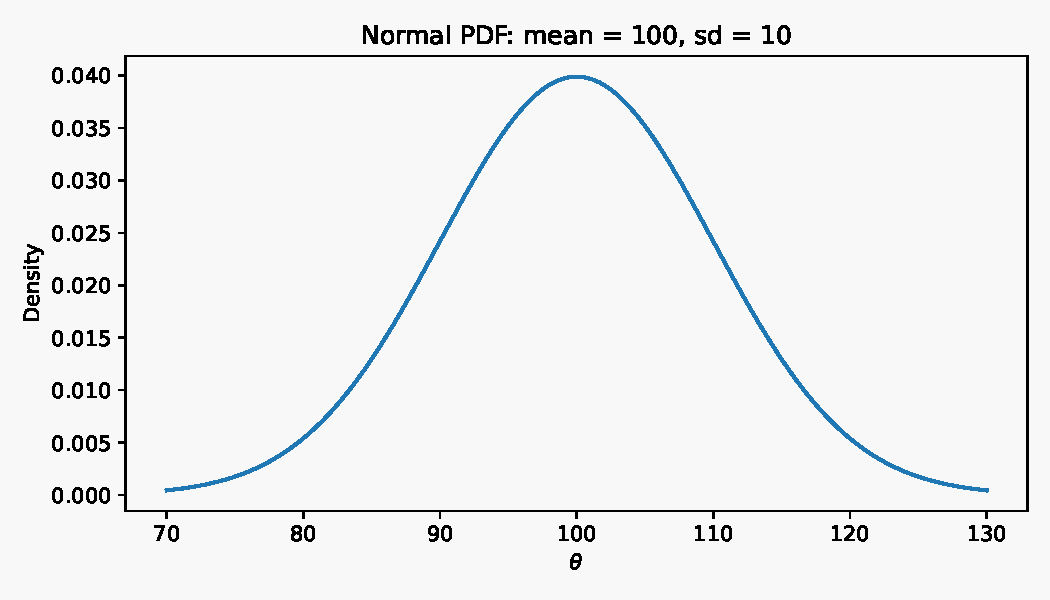
\includegraphics[keepaspectratio]{lectures/part2/6-bayes-inference_files/figure-pdf/unnamed-chunk-2-1.pdf}}
\end{center}

\subsection{R}

\begin{Shaded}
\begin{Highlighting}[]
\NormalTok{mean }\OtherTok{\textless{}{-}} \DecValTok{100}
\NormalTok{sd   }\OtherTok{\textless{}{-}} \DecValTok{10}

\NormalTok{theta\_grid }\OtherTok{\textless{}{-}} \FunctionTok{seq}\NormalTok{(mean }\SpecialCharTok{{-}} \DecValTok{3}\SpecialCharTok{*}\NormalTok{sd, mean }\SpecialCharTok{+} \DecValTok{3}\SpecialCharTok{*}\NormalTok{sd, }\AttributeTok{length.out =} \DecValTok{200}\NormalTok{)}
\NormalTok{pdf\_values }\OtherTok{\textless{}{-}} \FunctionTok{dnorm}\NormalTok{(theta\_grid, }\AttributeTok{mean =}\NormalTok{ mean, }\AttributeTok{sd =}\NormalTok{ sd)}

\FunctionTok{plot}\NormalTok{(theta\_grid, pdf\_values, }\AttributeTok{type =} \StringTok{"l"}\NormalTok{,}
     \AttributeTok{xlab =} \FunctionTok{expression}\NormalTok{(theta),}
     \AttributeTok{ylab =} \StringTok{"Density"}\NormalTok{,}
     \AttributeTok{main =} \StringTok{"Normal PDF: mean = 100, sd = 10"}\NormalTok{)}
\end{Highlighting}
\end{Shaded}

\begin{center}
\pandocbounded{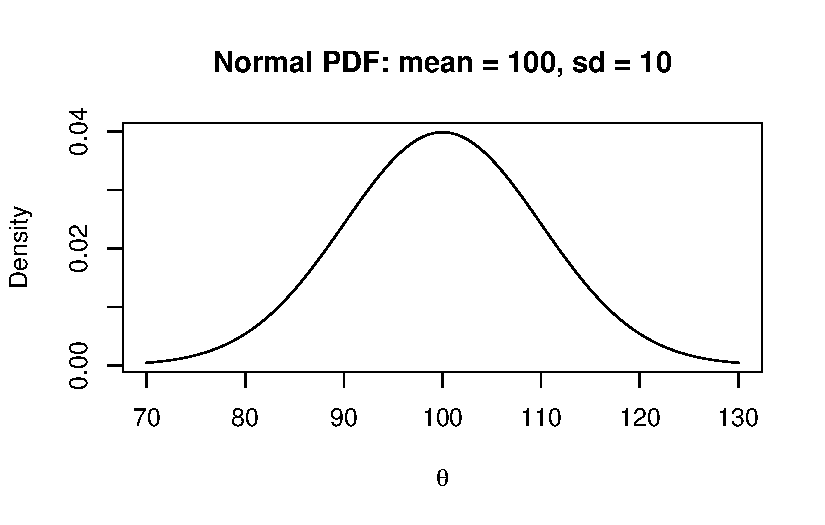
\includegraphics[keepaspectratio]{lectures/part2/6-bayes-inference_files/figure-pdf/unnamed-chunk-3-3.pdf}}
\end{center}

\section{Bayes' Theorem}\label{bayes-theorem-1}

Bayesian inference takes its name from \textbf{Bayes' theorem}, which
tells us how to update our beliefs about \(\theta\) after seeing data.

Recall from probability that for events \(A\) and \(B\):

\[
\mathrm{Pr}(A \mid B) = \frac{\mathrm{Pr}(B \mid A)\,\mathrm{Pr}(A)}{\mathrm{Pr}(B)}.
\]

To generalise this idea to \textbf{random variables and densities}, we
use conditional densities:

\[
f_{X \mid Y}(x \mid y) = \frac{f_{XY}(x,y)}{f_Y(y)}.
\]

\begin{refremark}
\textbf{Notation.} We will usually write \(f(x \mid y)\) rather than
\(f_{X \mid Y}(x \mid y)\) to keep things simple. Both mean the same
thing.

\label{rem-notation}

\end{refremark}

Using this, we obtain Bayes' theorem for densities.

\begin{theorem}[Bayes' Theorem for
Densities.]\protect\hypertarget{thm-bayes}{}\label{thm-bayes}

For random variables \(X\) and \(Y\):

\[
f(x \mid y) = \frac{f(y \mid x)\,f(x)}{f(y)}.
\]

\end{theorem}

\begin{refproof}
By the definition of conditional density:

\[
f(x \mid y) = \frac{f(x,y)}{f(y)}, 
\qquad
f(y \mid x) = \frac{f(x,y)}{f(x)}.
\]

Rearranging the second expression gives \(f(x,y) = f(y \mid x) f(x)\).
Substituting this into the first gives

\[
f(x \mid y) = \frac{f(y \mid x) f(x)}{f(y)}.
\]

\label{prf-bayes}

\end{refproof}

\begin{center}\rule{0.5\linewidth}{0.5pt}\end{center}

\section{Bayes' Theorem in
Statistics}\label{bayes-theorem-in-statistics}

In Bayesian inference, we apply Bayes' theorem with:

\begin{itemize}
\tightlist
\item
  \(x = \theta\) (the parameter, treated as random),
\item
  \(y = \underline{x}\) (the observed data).
\end{itemize}

This gives:

\[
\pi(\theta \mid \underline{x}) 
= \frac{f(\underline{x} \mid \theta)\,\pi(\theta)}{f(\underline{x})}.
\]

\begin{definition}[Posterior
Distribution.]\protect\hypertarget{def-posterior}{}\label{def-posterior}

\[
\pi(\theta \mid \underline{x}) 
= \frac{f(\underline{x} \mid \theta)\,\pi(\theta)}{f(\underline{x})}.
\]

The \textbf{posterior} combines two ingredients:

\begin{itemize}
\tightlist
\item
  The \textbf{likelihood} \(f(\underline{x} \mid \theta)\) (information
  from the data).
\item
  The \textbf{prior} \(\pi(\theta)\) (information before seeing the
  data).
\end{itemize}

The denominator \(f(\underline{x})\) is a normalising constant ensuring
the posterior integrates to 1.

\end{definition}

\begin{tcolorbox}[enhanced jigsaw, left=2mm, colframe=quarto-callout-important-color-frame, toprule=.15mm, rightrule=.15mm, leftrule=.75mm, breakable, opacityback=0, arc=.35mm, colback=white, bottomrule=.15mm]

\vspace{-3mm}\textbf{✨ Big picture:}\vspace{3mm}

Bayesian inference updates prior beliefs about parameters using the
likelihood from the data, producing the posterior distribution which
represents \emph{updated uncertainty}.

\end{tcolorbox}

Let's start with a simple example to see how this works:

\begin{example}[Biased
Coin]\protect\hypertarget{exm-biased-coin}{}\label{exm-biased-coin}

We consider a possibly biased coin with parameter
\(\theta = \Pr(\text{Head})\). Before seeing data, we express \emph{no
preference} over \(\theta\in(0,1)\) via a uniform prior: \[
\theta \sim \mathrm{Uniform}(0,1) \equiv \mathrm{Beta}(1,1), \qquad \pi(\theta)=1 \ \text{for } 0<\theta<1.
\] Hence \(\mathrm{E}[\theta]=0.5\).

We toss the coin \(n=5\) times and observe \(x=1\) head. Find the
\textbf{posterior} \(\pi(\theta\mid x)\).

\end{example}

\begin{refsolution}
Let \(X\) be the number of heads in \(5\) tosses. Assuming that each
coin throw is \emph{independent and identically distributed}, \(X\) is
Binomial\footnote{\textbf{Binomial distribution.} If we assume each coin
  throw \(C_i\) is an i.i.d. \(\textrm{Bernoulli}(\theta)\) trial with a
  \(1\) representing a heads landing, and a \(0\) representing a tails,
  the total number of heads out of \(5\) is
  \(X = C_1 + C_2 + C_3 + C_4 + C_5\). Therefore: \[
      X \mid \theta \sim \textrm{Bin}(5,\theta).
  \]}: \[
    X \mid \theta \sim \textrm{Bin}(5,\theta).
\] Note that there is only a \textbf{single observation} here: one
experiment is ``tossing the coin \(5\) times and seeing how many come up
heads''. The probability of observing \(X=1\) is \[
    f(x = 1 \mid \theta) = 5\theta(1-\theta)^4
\] If we plot this:

\begin{Shaded}
\begin{Highlighting}[]
\ImportTok{import}\NormalTok{ matplotlib.pyplot }\ImportTok{as}\NormalTok{ plt}
\ImportTok{import}\NormalTok{ numpy }\ImportTok{as}\NormalTok{ np}
\ImportTok{import}\NormalTok{ math}

\KeywordTok{def}\NormalTok{ binom\_lik(theta):}
    \ControlFlowTok{return} \DecValTok{5} \OperatorTok{*}\NormalTok{ theta }\OperatorTok{*}\NormalTok{ (}\DecValTok{1} \OperatorTok{{-}}\NormalTok{ theta) }\OperatorTok{**} \DecValTok{4}


\NormalTok{theta\_grid }\OperatorTok{=}\NormalTok{ np.linspace(}\DecValTok{0}\NormalTok{, }\DecValTok{1}\NormalTok{, }\DecValTok{200}\NormalTok{)}
\NormalTok{binom\_lik\_vals }\OperatorTok{=}\NormalTok{ binom\_lik(theta\_grid)}

\NormalTok{plt.figure(figsize}\OperatorTok{=}\NormalTok{(}\DecValTok{5}\NormalTok{,}\DecValTok{3}\NormalTok{))}
\NormalTok{plt.plot(theta\_grid, binom\_lik\_vals)}
\NormalTok{plt.xlabel(}\VerbatimStringTok{r"}\DecValTok{$}\CharTok{\textbackslash{}t}\VerbatimStringTok{heta}\DecValTok{$}\VerbatimStringTok{"}\NormalTok{)}
\NormalTok{plt.ylabel(}\StringTok{"Likelihood"}\NormalTok{)}
\NormalTok{plt.title(}\StringTok{"Binomial Likelihood (with $n=5$ and $X=1$)"}\NormalTok{)}
\NormalTok{plt.tight\_layout()}
\NormalTok{plt.show()  }
\end{Highlighting}
\end{Shaded}

\begin{center}
\pandocbounded{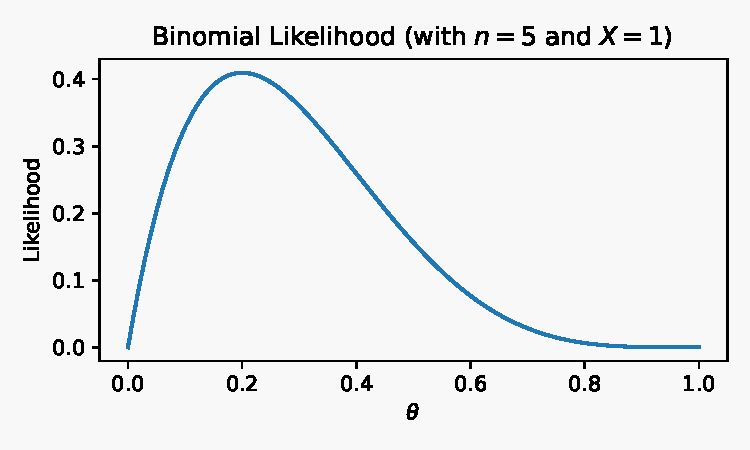
\includegraphics[keepaspectratio]{lectures/part2/6-bayes-inference_files/figure-pdf/unnamed-chunk-4-1.pdf}}
\end{center}

we see that this favours \(\theta\) around \(0.2\). In fact, in
Example~\ref{exm-binom-mle-single}, we saw that the MLE is
\(\hat{\theta} = 0.2\).

Our prior for \(\theta\) was \(\pi(\theta) = 1\), for
\(0 < \theta < 1\). To update our beliefs, by conditioning on the single
observation \(x=2\), we use {Bayes Theorem~\ref{def-posterior}}: \[
    \pi(\theta|x=1)=\frac{\pi(\theta)f(x=1|\theta)}{f(x=1)} = \frac{1 \times 5\theta(1-\theta)^4}{f(x=1)}, \quad 0 < \theta < 1.
\] To compute the \emph{denominator}, \(f(x=1)\), we use the {law of
total probability~\ref{thm-total-probability-pdfs}}:

\begin{align*}
f(x=1) &=\int_\Theta\pi(\theta)f(x=1\, |\,\theta)\,d\theta = \int_0^1 1\times 5\theta(1-\theta)^4\,d\theta \\
&=\int_0^1 \theta\times 5(1-\theta)^4\,d\theta =\left[-(1-\theta)^5\,\theta\right]^1_0
+\int_0^1 (1-\theta)^5\,d\theta \\
&=0 + \left[-\frac{(1-\theta)^6}{6}\right]^1_0 =\frac{1}{6}. 
\end{align*}

Therefore, the posterior density is (for \(0<\theta<1\)):

\begin{align*}
\pi(\theta|x=1)&=\frac{\pi(\theta)f(x=1|\theta)}{f(x=1)} =\frac{5\theta(1-\theta)^4}{1/6}\\
&=30\,\theta(1-\theta)^4 =\frac{\theta(1-\theta)^4}{\mathrm{B}(2,5)},\quad\quad 0<\theta<1,
\end{align*}

and so the posterior distribution is
\(\theta|x=1\sim \textrm{Beta}(2,5)\). This distribution has its mode at
\(\theta=0.2\), and mean at \(\mathrm{E}[\theta|x=1]=2/7=0.286\).

\label{sol-biased-coin}

\end{refsolution}

The main difficulty in calculating the posterior distribution was in
obtaining the \(f(x)\) term. However, in many cases we can recognise the
posterior distribution without the need to calculate this constant term
(constant with respect to \(\theta\)). In this example, we can calculate
the posterior distribution as

\begin{align*}
\pi(\theta|\underline{x})&\propto\pi(\theta)f(x=1|\theta) \\
&\propto 1\times 5\theta(1-\theta)^4,\quad\quad 0<\theta<1  \\
&=k\theta(1-\theta)^4,\quad\quad 0<\theta<1.
\end{align*}

As \(\theta\) is a continuous quantity, what we would like to know is
what continuous distribution defined on \((0,1)\) has a probability
density function which takes the form \(k\theta^{g-1}(1-\theta)^{h-1}\).
The answer is the \(\textrm{Beta}(g,h)\) distribution. Therefore,
choosing \(g\) and \(h\) appropriately, we can see that the posterior
distribution is \(\theta|x=1\sim \textrm{Beta}(2,5)\).

\textbf{Summary:}

It is possible that we have a biased coin. If we suppose that all values
of \(\theta=\text{Pr(Head)}\) are equally likely and then observe 1 head
out of 5, then the most likely value of \(\theta\) is 0.2 --- the same
as the most likely value from the data alone (not surprising!). However,
on average, we would expect \(\theta\) to be around 0.286. Uncertainty
about \(\theta\) has changed from a (prior) standard deviation of 0.289
to a (posterior) standard deviation of 0.160. The changes in our beliefs
about \(\theta\) are more fully described by the prior and posterior
distributions shown in \textbf{?@fig-beta-posterior}.

\begin{center}\rule{0.5\linewidth}{0.5pt}\end{center}

\begin{Shaded}
\begin{Highlighting}[]

\NormalTok{// Domain and grid}
\NormalTok{mDomain = [0, 1]}
\NormalTok{pdfXs = d3.scaleLinear().domain(mDomain).ticks(200)  // 201 points including 0 and 1}

\NormalTok{// PDFs (closed{-}form)}
\NormalTok{function priorPDF(x)     \{ return (x \textgreater{} 0 \&\& x \textless{} 1) ? 1 : 0; \}}
\NormalTok{function posteriorPDF(x) \{ return (x \textgreater{} 0 \&\& x \textless{} 1) ? 30 * x * (1 {-} x) ** 4 : 0; \}}

\NormalTok{// Data (use the scalar x from map!)}
\NormalTok{prior = pdfXs.map(x =\textgreater{} (\{ x, y: priorPDF(x), which: "Prior  Beta(1,1)" \}))}
\NormalTok{post  = pdfXs.map(x =\textgreater{} (\{ x, y: posteriorPDF(x), which: "Posterior  Beta(2,5)" \}))}
\end{Highlighting}
\end{Shaded}

\begin{Shaded}
\begin{Highlighting}[]
\NormalTok{//| label: fig{-}beta{-}posterior}
\NormalTok{//| fig{-}cap: Prior and posterior distributions for the coin bias parameter $\textbackslash{}theta=\textbackslash{}Pr(\textbackslash{}text\{Head\})$ after observing 1 head in 5 tosses. The posterior is more concentrated, reflecting reduced uncertainty about $\textbackslash{}theta$ compared to the uniform prior}
\NormalTok{//| fig{-}align: center}

\NormalTok{bodyFont = getComputedStyle(document.body).fontFamily}
\NormalTok{// Figure}
\NormalTok{viewof fig\_beta = Plot.plot(\{}
\NormalTok{  width: 640,}
\NormalTok{  height: 320,}
\NormalTok{  marginLeft: 48,}
\NormalTok{  marginBottom: 40,}
\NormalTok{  x: \{ label: "θ", domain: [0, 1] \},}
\NormalTok{  y: \{ label: "Density" \},}
\NormalTok{  style: \{ background: "var({-}{-}plot{-}panel{-}bg)", }
\NormalTok{           fontSize: 14,}
\NormalTok{           fontFamily: bodyFont,  \},}
\NormalTok{  marks: [}
\NormalTok{    Plot.ruleY([0], \{ stroke: "var({-}{-}border)", strokeOpacity: 0.6 \}),}
\NormalTok{    Plot.lineY(prior, \{ x: "x", y: "y", stroke: "var({-}{-}brand{-}red)",  strokeWidth: 2, strokeOpacity: 0.85 \}),}
\NormalTok{    Plot.areaY(prior, \{ x: "x", y: "y", fill: "var({-}{-}brand{-}red)", fillOpacity: 0.05 \}),}
\NormalTok{    Plot.lineY(post,  \{ x: "x", y: "y", stroke: "var({-}{-}brand{-}teal)", strokeWidth: 2 \}),}
\NormalTok{    Plot.areaY(post,  \{ x: "x", y: "y", fill: "var({-}{-}brand{-}teal)", fillOpacity: 0.2 \}),}
\NormalTok{    Plot.text(}
\NormalTok{      [}
\NormalTok{        \{ x: 0.8, y: priorPDF(0.8),     label: "Prior" \},}
\NormalTok{        \{ x: 0.35, y: posteriorPDF(0.3), label: "Posterior" \}}
\NormalTok{      ],}
\NormalTok{      \{ x: "x", y: "y", text: "label", dy: {-}8 \}}
\NormalTok{    )}
\NormalTok{  ]}
\NormalTok{\})}
\end{Highlighting}
\end{Shaded}

\begin{center}\rule{0.5\linewidth}{0.5pt}\end{center}

\begin{example}[]\protect\hypertarget{exm-music-expert}{}\label{exm-music-expert}

Consider an experiment to determine how good a music expert is at
distinguishing between pages from Haydn and Mozart scores. Let
\(\theta=\mathrm{Pr}(\text{correct choice})\). Suppose that, before
conducting the experiment, we have been told that the expert is very
competent. In fact, it is suggested that we should have a prior
distribution which has a mode around \(\theta=0.95\) and for which
\(\mathrm{Pr}(\theta<0.8)\) is very small. We choose
\(\theta\sim \textrm{Beta}(77,5)\), with probability density function \[
\pi(\theta)=128107980\,\theta^{76}(1-\theta)^4,\quad\quad 0<\theta<1.
\] A graph of this prior density is given as follows:

\subsection{Python}

\begin{Shaded}
\begin{Highlighting}[]
\ImportTok{import}\NormalTok{ numpy }\ImportTok{as}\NormalTok{ np}
\ImportTok{import}\NormalTok{ math}
\ImportTok{import}\NormalTok{ matplotlib.pyplot }\ImportTok{as}\NormalTok{ plt}

\CommentTok{\# Beta(α, β) with α=77, β=5  →  π(θ) ∝ θ\^{}(76) (1{-}θ)\^{}(4)}
\NormalTok{alpha, beta }\OperatorTok{=} \DecValTok{77}\NormalTok{, }\DecValTok{5}

\CommentTok{\# B(α,β) = Γ(α)Γ(β)/Γ(α+β)  ⇒  1/B = exp(lgamma(α+β) {-} lgamma(α) {-} lgamma(β))}
\CommentTok{\# Note the lgamma function computes the logarithm of the Gamma function.}
\NormalTok{beta\_const\_inv }\OperatorTok{=}\NormalTok{ math.exp(math.lgamma(alpha }\OperatorTok{+}\NormalTok{ beta) }\OperatorTok{{-}}\NormalTok{ math.lgamma(alpha) }\OperatorTok{{-}}\NormalTok{ math.lgamma(beta))}

\KeywordTok{def}\NormalTok{ beta\_pdf(theta):}
    \ControlFlowTok{return}\NormalTok{ beta\_const\_inv }\OperatorTok{*}\NormalTok{ np.power(theta, alpha }\OperatorTok{{-}} \DecValTok{1}\NormalTok{) }\OperatorTok{*}\NormalTok{ np.power(}\DecValTok{1} \OperatorTok{{-}}\NormalTok{ theta, beta }\OperatorTok{{-}} \DecValTok{1}\NormalTok{)}

\NormalTok{theta\_grid }\OperatorTok{=}\NormalTok{ np.linspace(}\FloatTok{0.0}\NormalTok{, }\FloatTok{1.0}\NormalTok{, }\DecValTok{500}\NormalTok{)}
\NormalTok{pdf\_values }\OperatorTok{=}\NormalTok{ beta\_pdf(theta\_grid)}

\NormalTok{plt.figure(figsize}\OperatorTok{=}\NormalTok{(}\DecValTok{7}\NormalTok{,}\DecValTok{4}\NormalTok{))}
\NormalTok{plt.plot(theta\_grid, pdf\_values)}
\NormalTok{plt.xlabel(}\VerbatimStringTok{r"}\DecValTok{$}\CharTok{\textbackslash{}t}\VerbatimStringTok{heta}\DecValTok{$}\VerbatimStringTok{"}\NormalTok{)}
\NormalTok{plt.ylabel(}\StringTok{"Density"}\NormalTok{)}
\NormalTok{plt.title(}\VerbatimStringTok{rf"Beta PDF: }\DecValTok{$}\CharTok{\textbackslash{}a}\VerbatimStringTok{lpha=}\SpecialCharTok{\{}\NormalTok{alpha}\SpecialCharTok{\}}\DecValTok{$}\VerbatimStringTok{, }\DecValTok{$\textbackslash{}b}\VerbatimStringTok{eta=}\SpecialCharTok{\{}\NormalTok{beta}\SpecialCharTok{\}}\DecValTok{$}\VerbatimStringTok{"}\NormalTok{)}
\CommentTok{\# plt.xlim(0, 1)}
\NormalTok{plt.tight\_layout()}
\NormalTok{plt.show()}
\end{Highlighting}
\end{Shaded}

\begin{center}
\pandocbounded{
\includegraphics[keepaspectratio]{lectures/part2/6-bayes-inference_files/figure-pdf/unnamed-chunk-7-3.pdf}}
\end{center}

\subsection{R}

\begin{Shaded}
\begin{Highlighting}[]
\NormalTok{alpha }\OtherTok{\textless{}{-}} \DecValTok{77}
\NormalTok{beta  }\OtherTok{\textless{}{-}} \DecValTok{5}

\CommentTok{\# Normalising constant via log{-}gamma (works like Python\textquotesingle{}s lgamma)}
\NormalTok{beta\_const\_inv }\OtherTok{\textless{}{-}} \FunctionTok{exp}\NormalTok{(}\FunctionTok{lgamma}\NormalTok{(alpha }\SpecialCharTok{+}\NormalTok{ beta) }\SpecialCharTok{{-}} \FunctionTok{lgamma}\NormalTok{(alpha) }\SpecialCharTok{{-}} \FunctionTok{lgamma}\NormalTok{(beta))}

\NormalTok{beta\_pdf }\OtherTok{\textless{}{-}} \ControlFlowTok{function}\NormalTok{(theta) \{}
\NormalTok{  beta\_const\_inv }\SpecialCharTok{*}\NormalTok{ theta}\SpecialCharTok{\^{}}\NormalTok{(alpha }\SpecialCharTok{{-}} \DecValTok{1}\NormalTok{) }\SpecialCharTok{*}\NormalTok{ (}\DecValTok{1} \SpecialCharTok{{-}}\NormalTok{ theta)}\SpecialCharTok{\^{}}\NormalTok{(beta }\SpecialCharTok{{-}} \DecValTok{1}\NormalTok{)}
\NormalTok{\}}

\NormalTok{theta\_grid }\OtherTok{\textless{}{-}} \FunctionTok{seq}\NormalTok{(}\DecValTok{0}\NormalTok{, }\DecValTok{1}\NormalTok{, }\AttributeTok{length.out =} \DecValTok{500}\NormalTok{)}
\NormalTok{pdf\_values }\OtherTok{\textless{}{-}} \FunctionTok{beta\_pdf}\NormalTok{(theta\_grid)}

\FunctionTok{plot}\NormalTok{(theta\_grid, pdf\_values, }\AttributeTok{type =} \StringTok{"l"}\NormalTok{,}
     \AttributeTok{xlab =} \FunctionTok{expression}\NormalTok{(theta), }\AttributeTok{ylab =} \StringTok{"Density"}\NormalTok{,}
     \AttributeTok{main =} \FunctionTok{bquote}\NormalTok{(}\StringTok{"Beta PDF: "} \SpecialCharTok{\textasciitilde{}}\NormalTok{ alpha }\SpecialCharTok{==}\NormalTok{ .(alpha) }\SpecialCharTok{\textasciitilde{}} \StringTok{","} \SpecialCharTok{\textasciitilde{}}\NormalTok{ beta }\SpecialCharTok{==}\NormalTok{ .(beta)))}
\end{Highlighting}
\end{Shaded}

\begin{center}
\pandocbounded{
\includegraphics[keepaspectratio]{lectures/part2/6-bayes-inference_files/figure-pdf/unnamed-chunk-8-5.pdf}}
\end{center}

\end{example}

\section{Bayesian vs.~Frequentist
(again)}\label{bayesian-vs.-frequentist-again}

\part{Part III - Interval Estimation}

\chapter{Frequentist Interval
Estimation}\label{frequentist-interval-estimation}

Recalling the {main inference tasks~\ref{sec-inference-tasks}}, we now
move from \emph{point estimation} to \emph{interval estimation}.

The key idea is that instead of giving a single ``best
guess''\footnote{Recall from Chapter~\ref{sec-bayes-inference} that
  Bayesians do not return a single ``best guess,'' but a full
  \textbf{posterior distribution} over parameter values. From this
  distribution we can compute \textbf{summaries} such as plausible
  ranges of \(\theta\) (see Chapter~\ref{sec-bayesian-intervals}), which
  play a role similar to confidence intervals but with a different
  interpretation.} of a parameter, we want to provide a \textbf{range of
plausible values}. In other words, an \textbf{interval}.

\section{The Frequentist Perspective}\label{the-frequentist-perspective}

Recall that, for frequentists, the parameter \(\theta\) is \textbf{fixed
but unknown}.

The randomness comes from the data: if we repeated the experiment many
times, we would get different samples, different estimates, and hence
different intervals.

\begin{itemize}
\tightlist
\item
  \textbf{Point Estimate:} a single statistic
  \(\hat{\theta}(\underline{X})\).
\item
  \textbf{Interval estimate:} two statistics \(L(\underline{X})\) and
  \(U(\underline{X})\) that form a \emph{random interval}.
\end{itemize}

\begin{definition}[Confidence
Interval]\protect\hypertarget{def-confidence-interval}{}\label{def-confidence-interval}

A \(100(1-\alpha)\%\) \textbf{confidence interval} for \(\theta\) is a
\emph{random interval} \[
\big[L(\underline{X}),\; U(\underline{X})\big]
\] satisfying \[
\mathrm{Pr} \big(L(\underline{X}) < \theta < U(\underline{X})\big) = 1 - \alpha.
\]

This property is called \textbf{coverage}: in the long run, a proportion
\(1-\alpha\) of such intervals (constructed from repeated experiments)
will contain the true \(\theta\).

\end{definition}

\begin{center}\rule{0.5\linewidth}{0.5pt}\end{center}

\textbf{Visualisation:} We

\begin{Shaded}
\begin{Highlighting}[]
\NormalTok{//| echo: false}

\NormalTok{/* {-}{-}{-}{-}{-}{-}{-}{-}{-}{-}{-}{-}{-}{-}{-}{-}{-}{-}{-}{-}{-}{-}{-}{-}{-}{-}{-}{-}{-}{-}{-}{-}{-}{-}{-}{-}{-}{-}{-}{-}{-}{-}{-}{-}{-}{-}{-}{-}{-}{-}{-}{-}{-}{-}{-}{-}{-}{-}{-}}
\NormalTok{   Confidence Intervals for μ (Normal data) — z{-}interval only}
\NormalTok{   Left: current sample + z{-}CI}
\NormalTok{   Right: true μ line + vertical z{-}CIs added on each resample}
\NormalTok{   {-}{-}{-}{-}{-}{-}{-}{-}{-}{-}{-}{-}{-}{-}{-}{-}{-}{-}{-}{-}{-}{-}{-}{-}{-}{-}{-}{-}{-}{-}{-}{-}{-}{-}{-}{-}{-}{-}{-}{-}{-}{-}{-}{-}{-}{-}{-}{-}{-}{-}{-}{-}{-}{-}{-}{-}{-}{-}{-} */}
\NormalTok{bodyFont = getComputedStyle(document.body).fontFamily}

\NormalTok{// {-}{-}{-}{-}{-}{-}{-}{-}{-}{-} Mutable state {-}{-}{-}{-}{-}{-}{-}{-}{-}{-}}
\NormalTok{mutable rngSeed = 1}
\NormalTok{mutable resampleClicks = 0}
\NormalTok{mutable resetClicks = 0}

\NormalTok{// history of z{-}intervals: array of \{L, U, covered\}}
\NormalTok{mutable ciZHistory = []}

\NormalTok{// last interval (to archive on next click)}
\NormalTok{mutable lastZ = null}


\NormalTok{// {-}{-}{-}{-}{-}{-}{-}{-}{-}{-} Buttons {-}{-}{-}{-}{-}{-}{-}{-}{-}{-}}
\NormalTok{function styledButton(label, cls, options = \{\}) \{}
\NormalTok{  const el = Inputs.button(label, options);}
\NormalTok{  const btn = el.querySelector(\textquotesingle{}button\textquotesingle{});}
\NormalTok{  if (btn) btn.classList.add(cls);}
\NormalTok{  return el;}
\NormalTok{\}}
\NormalTok{viewof resample = styledButton("Resample", "btn{-}resample", \{ reduce: c =\textgreater{} (c ?? 0) + 1 \})}
\NormalTok{viewof reset    = styledButton("Reset",    "btn{-}reset",    \{ reduce: c =\textgreater{} (c ?? 0) + 1 \})}

\NormalTok{// {-}{-}{-}{-}{-}{-}{-}{-}{-}{-} Edge triggers {-}{-}{-}{-}{-}{-}{-}{-}{-}{-}}
\NormalTok{\{}
\NormalTok{  if (reset \textgreater{} resetClicks) \{}
\NormalTok{    mutable ciZHistory = [];}
\NormalTok{    mutable lastZ = null;}
\NormalTok{    mutable resetClicks = reset;}
\NormalTok{  \}}
\NormalTok{  return html\textasciigrave{}\textasciigrave{};}
\NormalTok{\}}
\NormalTok{\{}
\NormalTok{  if (resample \textgreater{} resampleClicks) \{}
\NormalTok{    if (lastZ) \{}
\NormalTok{      mutable ciZHistory = [...ciZHistory, lastZ];}
\NormalTok{    \}}
\NormalTok{    mutable rngSeed = rngSeed + 1;}
\NormalTok{    mutable resampleClicks = resample;}
\NormalTok{  \}}
\NormalTok{  return html\textasciigrave{}\textasciigrave{};}
\NormalTok{\}}

\NormalTok{// {-}{-}{-}{-}{-}{-}{-}{-}{-}{-} Quantiles (z only) {-}{-}{-}{-}{-}{-}{-}{-}{-}{-}}
\NormalTok{qnorm = (p) =\textgreater{} \{}
\NormalTok{  if (p \textless{}= 0 || p \textgreater{}= 1) return NaN;}
\NormalTok{  const a = [{-}3.969683028665376e+01,2.209460984245205e+02,{-}2.759285104469687e+02,1.383577518672690e+02,{-}3.066479806614716e+01,2.506628277459239e+00];}
\NormalTok{  const b = [{-}5.447609879822406e+01,1.615858368580409e+02,{-}1.556989798598866e+02,6.680131188771972e+01,{-}1.328068155288572e+01];}
\NormalTok{  const c = [{-}7.784894002430293e{-}03,{-}3.223964580411365e{-}01,{-}2.400758277161838e+00,{-}2.549732539343734e+00,4.374664141464968e+00,2.938163982698783e+00];}
\NormalTok{  const d = [ 7.784695709041462e{-}03, 3.224671290700398e{-}01, 2.445134137142996e+00, 3.754408661907416e+00];}
\NormalTok{  const plow = 0.02425, phigh = 1 {-} plow;}
\NormalTok{  let q, r, x;}
\NormalTok{  if (p \textless{} plow) \{ q = Math.sqrt({-}2*Math.log(p));}
\NormalTok{    x = (((((c[0]*q+c[1])*q+c[2])*q+c[3])*q+c[4])*q+c[5]) / ((((d[0]*q+d[1])*q+d[2])*q+d[3])*q+1);}
\NormalTok{  \} else if (phigh \textless{} p) \{ q = Math.sqrt({-}2*Math.log(1{-}p));}
\NormalTok{    x = {-}(((((c[0]*q+c[1])*q+c[2])*q+c[3])*q+c[4])*q+c[5]) / ((((d[0]*q+d[1])*q+d[2])*q+d[3])*q+1);}
\NormalTok{  \} else \{ q = p {-} 0.5; r = q*q;}
\NormalTok{    x = (((((a[0]*r+a[1])*r+a[2])*r+a[3])*r+a[4])*r+a[5])*q / (((((b[0]*r+b[1])*r+b[2])*r+b[3])*r+b[4])*r+1);}
\NormalTok{  \}}
\NormalTok{  const erf = x =\textgreater{} \{ const s=Math.sign(x); x=Math.abs(x); const t=1/(1+0.5*x);}
\NormalTok{    const tau=t*Math.exp({-}x*x{-}1.26551223+1.00002368*t+0.37409196*t**2+0.09678418*t**3{-}0.18628806*t**4+0.27886807*t**5{-}1.13520398*t**6+1.48851587*t**7{-}0.82215223*t**8+0.17087277*t**9);}
\NormalTok{    return s*(1{-}tau);}
\NormalTok{  \};}
\NormalTok{  const SQRT2 = Math.SQRT2, SQRT2PI = Math.sqrt(2*Math.PI);}
\NormalTok{  const e = 0.5 * (1 + erf(x / SQRT2)) {-} p;}
\NormalTok{  const u = e * SQRT2PI * Math.exp(0.5 * x * x);}
\NormalTok{  return x {-} u / (1 + x * u);}
\NormalTok{\}}

\NormalTok{// {-}{-}{-}{-}{-}{-}{-}{-}{-}{-} Sample + statistics {-}{-}{-}{-}{-}{-}{-}{-}{-}{-}}
\NormalTok{X = \{}
\NormalTok{  const r = d3.randomNormal.source(d3.randomLcg(rngSeed))(controls.trueMu, controls.trueSigma);}
\NormalTok{  return d3.range(controls.n).map(r);}
\NormalTok{\}}
\NormalTok{xbar = d3.mean(X)}

\NormalTok{alpha = controls.alpha}
\NormalTok{zcrit = qnorm(1 {-} alpha/2)}

\NormalTok{// z–CI for μ (known σ)}
\NormalTok{ciZ = (\{}
\NormalTok{  L: xbar {-} zcrit * (controls.trueSigma / Math.sqrt(controls.n)),}
\NormalTok{  U: xbar + zcrit * (controls.trueSigma / Math.sqrt(controls.n))}
\NormalTok{\})}

\NormalTok{covers = (ci, theta) =\textgreater{} (ci.L \textless{}= theta \&\& theta \textless{}= ci.U);}
\NormalTok{currentCoveredZ = covers(ciZ, controls.trueMu);}

\NormalTok{// save current z so *next* resample archives it}
\NormalTok{\{}
\NormalTok{  mutable lastZ = \{ ...ciZ, covered: currentCoveredZ \};}
\NormalTok{  return html\textasciigrave{}\textasciigrave{}; // suppresses any output}
\NormalTok{\}}


\NormalTok{// {-}{-}{-}{-}{-}{-}{-}{-}{-}{-} Toolbar (above plots) {-}{-}{-}{-}{-}{-}{-}{-}{-}{-}}

\NormalTok{// {-}{-}{-}{-}{-}{-}{-}{-}{-}{-} Left panel: data + current z{-}CI {-}{-}{-}{-}{-}{-}{-}{-}{-}{-}}
\NormalTok{makeDensityReducer = (total) =\textgreater{} (values, extent) =\textgreater{}}
\NormalTok{  values.length / Math.max(1, total) / Math.max(1e{-}9, extent.x2 {-} extent.x1);}

\NormalTok{xExtent = d3.extent(X)}
\NormalTok{xPad    = 3 * controls.trueSigma}
\NormalTok{xDomain = [xExtent[0] {-} 0.1*(xPad||1), xExtent[1] + 0.1*(xPad||1)]}

\NormalTok{bins = d3.bin().domain(xDomain).thresholds(controls.bins)(X);}
\NormalTok{densities = bins.map(b =\textgreater{} (b.length / Math.max(1, controls.n)) / Math.max(1e{-}9, (b.x1 {-} b.x0)));}
\NormalTok{yMax = Math.max(0.05, d3.max(densities) ?? 0.05);}
\NormalTok{yCI  = yMax * 0.75}

\NormalTok{leftPlot = Plot.plot(\{}
\NormalTok{  width: Math.min(680, Math.max(360, width/2 {-} 20)),}
\NormalTok{  height: 340,}
\NormalTok{  style: \{ background: "var({-}{-}plot{-}panel{-}bg)",}
\NormalTok{           color: "var({-}{-}brand{-}fg)",}
\NormalTok{           fontFamily: bodyFont, }
\NormalTok{           fontSize: 14.}
\NormalTok{  \}, }
\NormalTok{  x: \{ label: "Data", domain: xDomain \},}
\NormalTok{  y: \{ label: "Density" \},}
\NormalTok{  marks: [}
\NormalTok{    Plot.rectY(X, Plot.binX(\{ y: makeDensityReducer(controls.n) \}, \{ x: d=\textgreater{}d, thresholds: controls.bins, inset: 0, fillOpacity: 0.4, fill: "var({-}{-}brand{-}teal)" \})),}
\NormalTok{    Plot.ruleX(X, \{ y1: 0, y2: yMax*0.05, stroke: "var({-}{-}brand{-}teal)", strokeWidth: 3, strokeOpacity: 1 \}),}
\NormalTok{    Plot.ruleX([controls.trueMu], \{ stroke: "var({-}{-}brand{-}purple)", strokeDasharray: "4,3", strokeWidth: 2 \}),}
\NormalTok{    Plot.ruleX([xbar], \{ stroke: "currentColor", strokeDasharray: "2,2" \}),}
\NormalTok{    Plot.dot([\{x:xbar,y:0\}], \{x:"x",y:"y", r:3, fill:"currentColor"\}),}

\NormalTok{    // current z–CI (horizontal link)}
\NormalTok{    Plot.link([\{x1:ciZ.L, x2:ciZ.U, y1:yCI, y2:yCI\}],}
\NormalTok{      \{ x1:"x1", x2:"x2", y1:"y1", y2:"y2", stroke:"var({-}{-}brand{-}orange)", strokeWidth:4 \}),}
\NormalTok{    Plot.dot([\{x:xbar,y:yCI\}], \{x:"x", y:"y", r:3, fill:"var({-}{-}brand{-}orange)"\}),}
\NormalTok{    Plot.text([\{x:(ciZ.L+ciZ.U)/2, y:yCI + 0.05*yMax, label:\textasciigrave{}CI ($\{((1{-}alpha)*100)|0\}\%)\textasciigrave{}\}],}
\NormalTok{      \{x:"x",y:"y",text:"label", dy:{-}4, fontSize:10, fill:"var({-}{-}brand{-}orange)"\}),}

\NormalTok{    Plot.ruleY([0])}
\NormalTok{  ]}
\NormalTok{\})}

\NormalTok{// {-}{-}{-}{-}{-}{-}{-}{-}{-}{-} Right panel: history as vertical z{-}CI segments {-}{-}{-}{-}{-}{-}{-}{-}{-}{-}}
\NormalTok{zHistory   = ciZHistory}
\NormalTok{indices    = d3.range(1, zHistory.length + 1)}
\NormalTok{coverageZ  = zHistory.length ? d3.mean(zHistory, d =\textgreater{} d.covered) : NaN}

\NormalTok{rightYDomain = (() =\textgreater{} \{}
\NormalTok{  const vals = [}
\NormalTok{    controls.trueMu,}
\NormalTok{    ...zHistory.flatMap(d =\textgreater{} [d.L, d.U]),}
\NormalTok{    ciZ.L, ciZ.U}
\NormalTok{  ];}
\NormalTok{  const lo = d3.min(vals), hi = d3.max(vals);}
\NormalTok{  const pad = 0.08 * (hi {-} lo || 1);}
\NormalTok{  return [lo {-} pad, hi + pad];}
\NormalTok{\})()}

\NormalTok{rightPlot = Plot.plot(\{}
\NormalTok{  width: Math.min(680, Math.max(360, width/2 {-} 20)),}
\NormalTok{  height: 340,}
\NormalTok{  style: \{ background: "var({-}{-}plot{-}panel{-}bg)",}
\NormalTok{           color: "var({-}{-}brand{-}fg)",}
\NormalTok{           fontFamily: bodyFont, }
\NormalTok{           fontSize: 14.}
\NormalTok{  \}, }
\NormalTok{  x: \{ label: "Number of samples taken", domain: [0.5, Math.max(1.5, indices.length + 1.5)] \},}
\NormalTok{  y: \{ label: "μ", domain: rightYDomain \},}
\NormalTok{  marks: [}
\NormalTok{    Plot.ruleY([controls.trueMu], \{ stroke: "var({-}{-}brand{-}purple)", strokeDasharray: "4,3", strokeWidth: 2 \}),}

\NormalTok{    // archived z{-}CIs}
\NormalTok{    Plot.ruleX(zHistory.map((d,i)=\textgreater{}(\{x:i+1, y1:d.L, y2:d.U, covered:d.covered\})),}
\NormalTok{               \{ x:"x", y1:"y1", y2:"y2", stroke:(d)=\textgreater{} d.covered ? "var({-}{-}brand{-}orange)" : "\#999", strokeWidth: 3, opacity: 0.9 \}),}

\NormalTok{    // current interval (ghosted) at the next x{-}position}
\NormalTok{    Plot.ruleX([\{x:indices.length+1, y1:ciZ.L, y2:ciZ.U\}],}
\NormalTok{               \{ x:"x", y1:"y1", y2:"y2", stroke:"var({-}{-}brand{-}orange)", strokeWidth: 3, strokeOpacity:0.4 \}),}

\NormalTok{    // coverage text}
\NormalTok{    Plot.text(}
\NormalTok{      [\{x: 0.7, y: rightYDomain[1], label: \textasciigrave{}z{-}CI coverage: $\{isNaN(coverageZ) ? "—" : \textasciigrave{}$\{(100*coverageZ).toFixed(0)\}\%\textasciigrave{}\} ($\{zHistory.length\})\textasciigrave{}\}],}
\NormalTok{      \{x:"x", y:"y", text:"label", dx: 4, dy: 4, textAnchor: "start", fontSize: 11\}}
\NormalTok{    )}
\NormalTok{  ]}
\NormalTok{\})}

\NormalTok{\{}
\NormalTok{  // Make the forms behave nicely in the grid}
\NormalTok{  for (const f of [viewof resample, viewof reset]) \{}
\NormalTok{    f.style.margin = "0";}
\NormalTok{    f.style.width = "100\%";}
\NormalTok{    f.style.maxWidth = "none";}
\NormalTok{    f.style.display = "flex";}
\NormalTok{  \}}
\NormalTok{  viewof resample.style.justifyContent = "flex{-}start";}
\NormalTok{  viewof reset.style.justifyContent    = "flex{-}end";}

\NormalTok{  return html\textasciigrave{}\textless{}div class="ojs{-}toolbar{-}grid"\textgreater{}}
\NormalTok{    \textless{}div class="left"\textgreater{}$\{viewof resample\}\textless{}/div\textgreater{}}
\NormalTok{      \textless{}div class="center"\textgreater{}}
\NormalTok{        $\{md\textasciigrave{}$\{tex\textasciigrave{}\textbackslash{}big[L(\textbackslash{}underline\{X\}),\textbackslash{}, U(\textbackslash{}underline\{X\})\textbackslash{}big] = \textbackslash{}big[$\{ciZ.L.toFixed(2)\},\textbackslash{}; $\{ciZ.U.toFixed(2)\}\textbackslash{}big]\textasciigrave{}\}\textasciigrave{}\}}
\NormalTok{      \textless{}/div\textgreater{}}
\NormalTok{    \textless{}div class="right"\textgreater{}$\{viewof reset\}\textless{}/div\textgreater{}}
\NormalTok{  \textless{}/div\textgreater{}}

\NormalTok{  \textless{}style\textgreater{}}
\NormalTok{    .ojs{-}toolbar{-}grid\{}
\NormalTok{      display:grid;}
\NormalTok{      grid{-}template{-}columns:1fr auto 1fr; /* left, middle, right */}
\NormalTok{      align{-}items:center;}
\NormalTok{      width:100\%;}
\NormalTok{      box{-}sizing:border{-}box;}
\NormalTok{      margin:0; padding:0;}
\NormalTok{    \}}
\NormalTok{    .ojs{-}toolbar{-}grid form\{}
\NormalTok{      margin:0 !important;}
\NormalTok{      width:100\% !important;}
\NormalTok{      max{-}width:none !important;}
\NormalTok{      display:flex !important;}
\NormalTok{    \}}
\NormalTok{    .ojs{-}toolbar{-}grid .left  form\{ justify{-}content:flex{-}start !important; \}}
\NormalTok{    .ojs{-}toolbar{-}grid .right form\{ justify{-}content:flex{-}end   !important; \}}

\NormalTok{    .btn.btn{-}resample\{ background: var({-}{-}brand{-}teal); color:\#fff; border:none; \}}
\NormalTok{    .btn.btn{-}resample:hover\{ background: var({-}{-}brand{-}teal{-}hover); \}}
\NormalTok{    .btn.btn{-}reset\{ background: var({-}{-}brand{-}red); color:\#fff; border:none; \}}
\NormalTok{    .btn.btn{-}reset:hover\{ background: var({-}{-}brand{-}red{-}hover); \}}
\NormalTok{    .btn.btn{-}resample:focus{-}visible,}
\NormalTok{    .btn.btn{-}reset:focus{-}visible\{}
\NormalTok{      outline: 2px solid currentColor;}
\NormalTok{      outline{-}offset: 2px;}
\NormalTok{    \}}

\NormalTok{    .ojs{-}toolbar{-}grid .center\{}
\NormalTok{      text{-}align:center;}
\NormalTok{      font{-}size:0.9rem;}
\NormalTok{      color: var({-}{-}brand{-}fg);}
\NormalTok{    \}}
\NormalTok{  \textless{}/style\textgreater{}\textasciigrave{};}
\NormalTok{\}}

\NormalTok{html\textasciigrave{}\textless{}div style="max{-}width:100\%; display:flex; gap:14px; align{-}items:flex{-}start; flex{-}wrap:nowrap;"\textgreater{}}
\NormalTok{  \textless{}div\textgreater{}$\{leftPlot\}\textless{}/div\textgreater{}}
\NormalTok{  \textless{}div\textgreater{}$\{rightPlot\}\textless{}/div\textgreater{}}
\NormalTok{\textless{}/div\textgreater{}\textasciigrave{}}

\end{Highlighting}
\end{Shaded}

\begin{Shaded}
\begin{Highlighting}[]
\NormalTok{// {-}{-}{-}{-}{-}{-}{-}{-}{-}{-} Controls (to be rendered *below* the plots) {-}{-}{-}{-}{-}{-}{-}{-}{-}{-}}
\NormalTok{html\textasciigrave{}\textless{}style\textgreater{}}
\NormalTok{details.controls{-}root \textgreater{} summary \{}
\NormalTok{  list{-}style: none; cursor: pointer; user{-}select: none;}
\NormalTok{  background: var({-}{-}surface);}
\NormalTok{  border: 1px solid var({-}{-}border);}
\NormalTok{  border{-}radius: 10px;}
\NormalTok{  padding: 8px 10px;}
\NormalTok{  font{-}weight: 600; font{-}size: 13px;}
\NormalTok{  color: var({-}{-}fg{-}strong);}
\NormalTok{  display: flex; align{-}items: center; gap: 8px;}
\NormalTok{\}}
\NormalTok{/* {-}{-}{-}{-}{-}{-}{-}{-}{-}{-} Compact Inputs (fixed slider alignment) {-}{-}{-}{-}{-}{-}{-}{-}{-}{-} */}
\NormalTok{.controls{-}col label \{ font{-}size: 12px !important; \}}

\NormalTok{details.controls{-}root \textgreater{} summary::{-}webkit{-}details{-}marker \{ display: none; \}}
\NormalTok{details.controls{-}root[open] \textgreater{} summary \{ border{-}bottom{-}left{-}radius: 0; border{-}bottom{-}right{-}radius: 0; \}}
\NormalTok{details.controls{-}root \textgreater{} summary::before \{}
\NormalTok{  content: ""; display: inline{-}block; margin{-}right: 8px; width: 0; height: 0;}
\NormalTok{  border{-}style: solid; border{-}width: 3px 0 3px 6px;}
\NormalTok{  border{-}color: transparent transparent transparent var({-}{-}fg{-}strong);}
\NormalTok{  transform: rotate(0deg); transform{-}origin: 3px 50\%; transition: transform 60ms ease;}
\NormalTok{\}}
\NormalTok{details.controls{-}root[open] \textgreater{} summary::before \{ transform: rotate(90deg); \}}
\NormalTok{.controls{-}grid \{}
\NormalTok{  display: grid;}
\NormalTok{  grid{-}template{-}columns: minmax(260px,1fr) minmax(260px,1fr);}
\NormalTok{  gap: 12px;}
\NormalTok{  border: 1px solid var({-}{-}border); border{-}top: none;}
\NormalTok{  border{-}bottom{-}left{-}radius: 10px; border{-}bottom{-}right{-}radius: 10px;}
\NormalTok{  padding: 10px;}
\NormalTok{  background: var({-}{-}surface{-}weak);}
\NormalTok{\}}
\NormalTok{.controls{-}col \{ min{-}width: 260px; \}}
\NormalTok{.controls{-}col h4 \{}
\NormalTok{  margin: 0 0 6px 0; font{-}size: 12px; font{-}weight: 700;}
\NormalTok{  color: var({-}{-}fg{-}muted);}
\NormalTok{\}}
\NormalTok{.controls{-}col input[type="range"]\{ width:100\%; accent{-}color: var({-}{-}brand{-}teal,\#55C3CB); \}}

\NormalTok{/* Toolbar + buttons */}
\NormalTok{.btn.btn{-}resample\{ background: var({-}{-}brand{-}teal); color:\#fff; border:none; padding:6px 10px; border{-}radius:8px;\}}
\NormalTok{.btn.btn{-}resample:hover\{ background: var({-}{-}brand{-}teal{-}hover,\#4da2a8); \}}
\NormalTok{.btn.btn{-}reset\{ background: var({-}{-}brand{-}red,\#e65660); color:\#fff; border:none; padding:6px 10px; border{-}radius:8px;\}}
\NormalTok{.btn.btn{-}reset:hover\{ background: var({-}{-}brand{-}red{-}hover,\#bd4a52); \}}
\NormalTok{.toolbar\{ display:grid; grid{-}template{-}columns:1fr auto 1fr; align{-}items:center; gap:8px; margin: 6px 0 10px; \}}
\NormalTok{.toolbar .left form\{ display:flex; justify{-}content:flex{-}start; margin:0 \}}
\NormalTok{.toolbar .right form\{ display:flex; justify{-}content:flex{-}end;   margin:0 \}}
\NormalTok{.toolbar .center\{ text{-}align:center; font{-}size:0.9rem; color:var({-}{-}brand{-}fg) \}}

\NormalTok{/* Plots container: force side{-}by{-}side; scroll if too narrow */}
\NormalTok{.ci{-}row \{}
\NormalTok{  display: flex; gap: 14px; align{-}items: flex{-}start;}
\NormalTok{  flex{-}wrap: nowrap; overflow{-}x: auto; max{-}width: 100\%;}
\NormalTok{\}}
\NormalTok{.ci{-}panel \{ flex: 0 0 50\%; min{-}width: 460px; \}}
\NormalTok{\textless{}/style\textgreater{}\textasciigrave{}}

\NormalTok{viewof controls = \{}
\NormalTok{  const left = Inputs.form(\{}
\NormalTok{    n: Inputs.range([2, 400], \{ value: 20, step: 1, label: md\textasciigrave{}$\{tex\textasciigrave{}n\textasciigrave{}\}\textasciigrave{} \}),}
\NormalTok{    trueMu: Inputs.range([{-}2, 2], \{ value: 0, step: 0.1, label: md\textasciigrave{}$\{tex\textasciigrave{}\textbackslash{}mu\_\{\textbackslash{}text\{true\}\}\textasciigrave{}\}\textasciigrave{} \}),}
\NormalTok{    trueSigma: Inputs.range([0.3, 3], \{ value: 1, step: 0.1, label: md\textasciigrave{}$\{tex\textasciigrave{}\textbackslash{}sigma\textbackslash{} \textbackslash{}text\{(known)\}\textasciigrave{}\}\textasciigrave{} \})}
\NormalTok{  \}, \{ submit: false \});}

\NormalTok{  const right = Inputs.form(\{}
\NormalTok{    alpha: Inputs.range([0.01, 0.2], \{ value: 0.05, step: 0.01, label: md\textasciigrave{}$\{tex\textasciigrave{}\textbackslash{}alpha\textbackslash{} \textbackslash{}text\{(1−\}\textbackslash{}alpha\textbackslash{}text\{ confidence)\}\textasciigrave{}\}\textasciigrave{} \}),}
\NormalTok{    bins: Inputs.range([10, 60], \{ value: 24, step: 1, label: "Histogram bins" \})\});}

\NormalTok{  const root = html\textasciigrave{}\textless{}details class="controls{-}root" open\textgreater{}}
\NormalTok{    \textless{}summary\textgreater{}Simulation controls\textless{}/summary\textgreater{}}
\NormalTok{    \textless{}div class="controls{-}grid"\textgreater{}}
\NormalTok{      \textless{}div class="controls{-}col"\textgreater{}\textless{}h4\textgreater{}Data \& truth\textless{}/h4\textgreater{}\textless{}/div\textgreater{}}
\NormalTok{      \textless{}div class="controls{-}col"\textgreater{}\textless{}h4\textgreater{}Confidence level \& display\textless{}/h4\textgreater{}\textless{}/div\textgreater{}}
\NormalTok{    \textless{}/div\textgreater{}}
\NormalTok{  \textless{}/details\textgreater{}\textasciigrave{};}
\NormalTok{  root.querySelector(".controls{-}grid").children[0].append(left);}
\NormalTok{  root.querySelector(".controls{-}grid").children[1].append(right);}

\NormalTok{  const getValue = () =\textgreater{} (\{ ...left.value, ...right.value \});}
\NormalTok{  const update = () =\textgreater{} \{ root.value = getValue(); root.dispatchEvent(new CustomEvent("input", \{ bubbles: true \})); \};}
\NormalTok{  left.addEventListener("input", update);}
\NormalTok{  right.addEventListener("input", update);}
\NormalTok{  queueMicrotask(update);}
\NormalTok{  return root;}
\NormalTok{\}}
\end{Highlighting}
\end{Shaded}

\section{Interpreting Confidence
Intervals}\label{interpreting-confidence-intervals}

In practice, we only ever \textbf{observe one dataset}
\(\underline{x}\). So we calculate the observed interval: \[
[L_{\text{obs}}, U_{\text{obs}}] 
= \big[L(\underline{x}), U(\underline{x})\big].
\]

\begin{tcolorbox}[enhanced jigsaw, left=2mm, toprule=.15mm, breakable, opacityback=0, titlerule=0mm, toptitle=1mm, colbacktitle=quarto-callout-important-color!10!white, colframe=quarto-callout-important-color-frame, coltitle=black, rightrule=.15mm, leftrule=.75mm, bottomrule=.15mm, arc=.35mm, bottomtitle=1mm, title=\textcolor{quarto-callout-important-color}{\faExclamation}\hspace{0.5em}{Confidence Interval Interpretation}, colback=white, opacitybacktitle=0.6]

Once the data are observed, this interval is \textbf{fixed, not random}.

Therefore, a frequentist would \textbf{not} say \[
\mathrm{Pr}(L_{\text{obs}} < \theta < U_{\text{obs}}) = 1 - \alpha.
\] That statement is meaningless, because \(\theta\) is not random in
the frequentist view.

Instead, the correct interpretation is: \textbf{our method has long-run
coverage \(1-\alpha\).}

\end{tcolorbox}

\section{Deriving Confidence
Intervals}\label{deriving-confidence-intervals}

A \textbf{confidence interval (CI)} is a random interval, constructed
from the data, that is designed to contain the true value of a parameter
with a specified probability (the \emph{coverage probability}).

\begin{itemize}
\tightlist
\item
  If the coverage is exactly equal to the nominal level (e.g.~95\%), the
  CI is called \textbf{exact} or \textbf{well-calibrated}.
\item
  If the coverage only holds approximately (often as the sample size
  \(n \to \infty\)), the CI is called an \textbf{approximate interval}.
\end{itemize}

In practice, exact intervals are rare, but for certain classical models
(especially the normal distribution), we can derive them in closed form.

\subsection{The Normal Case (Known
Variance)}\label{the-normal-case-known-variance}

Suppose we observe \(n\) i.i.d. samples from a normal distribution with
\emph{known} variance \(\sigma^2\):

\[
X_i \sim \mathcal{N}(\mu, \sigma^2), \quad i=1,\dots,n.
\]

We want to construct a confidence interval for the unknown mean \(\mu\).

\subsubsection{Step 1: Sampling distribution of the
mean}\label{step-1-sampling-distribution-of-the-mean}

The sample mean is

\[
\bar{X} = \frac{1}{n}\sum_{i=1}^n X_i.
\]

Because the \(X\_i\) are normal, their average is also normal:

\[
\bar{X} \sim \mathcal{N}\!\left(\mu, \tfrac{\sigma^2}{n}\right).
\]

\subsubsection{Step 2: Standardisation}\label{step-2-standardisation}

Subtract the mean and divide by its standard deviation:

\[
Z = \frac{\bar{X} - \mu}{\sigma/\sqrt{n}}.
\]

This is exactly standard normal:

\[
Z \sim \mathcal{N}(0,1).
\]

\subsubsection{Step 3: Quantiles}\label{step-3-quantiles}

The middle \(1-\alpha\) probability mass of a standard normal is between
\(-z\_{1-\alpha/2}\) and \(z\_{1-\alpha/2}\), where \(z\_{1-\alpha/2}\)
is the \((1-\alpha/2)\) quantile. Thus,

\[
\Pr\!\left(-z_{1-\alpha/2} \leq \frac{\bar{X}-\mu}{\sigma/\sqrt{n}} \leq z_{1-\alpha/2}\right) = 1-\alpha.
\]

Rearranging gives the \textbf{exact \((1-\alpha)\) confidence interval}:

\[
\mu \in \biggl[\,\bar{X} - z_{1-\alpha/2}\,\frac{\sigma}{\sqrt{n}}, \;\; \bar{X} + z_{1-\alpha/2}\,\frac{\sigma}{\sqrt{n}} \,\biggr].
\]

Or equivalently:

\[
\bar{X} \;\pm\; z_{1-\alpha/2}\,\frac{\sigma}{\sqrt{n}}.
\]

\subsection{Normal Case (Unknown
Variance)}\label{normal-case-unknown-variance}

In practice, \(\sigma^2\) is almost never known. Instead, we estimate it
with the \textbf{sample variance}:

\[
S^2 = \frac{1}{n-1}\sum_{i=1}^n (X_i - \bar{X})^2.
\]

Replacing \(\sigma\) with \(S\) changes the distribution of our test
statistic.

\subsubsection{\texorpdfstring{Step 1: Distribution of the \(t\)
statistic}{Step 1: Distribution of the t statistic}}\label{step-1-distribution-of-the-t-statistic}

Define

\[
T = \frac{\bar{X} - \mu}{S/\sqrt{n}}.
\]

It can be shown (using properties of the chi-squared distribution and
independence between \(\bar{X}\) and \(S^2\)) that:

\[
T \sim t_{n-1},
\]

the \textbf{Student's \(t\) distribution} with \(n-1\) degrees of
freedom.

\begin{center}\rule{0.5\linewidth}{0.5pt}\end{center}

\subsubsection{\texorpdfstring{Aside: The Student's \(t\)
Distribution}{Aside: The Student's t Distribution}}\label{aside-the-students-t-distribution}

\begin{itemize}
\item
  The \(t\) distribution was discovered by William Sealy Gosset in 1908,
  under the pseudonym \emph{``Student''}.
\item
  It arises when a standard normal random variable is divided by the
  square root of an independent chi-squared variable divided by its
  degrees of freedom:

  \[
  T = \frac{Z}{\sqrt{U/\nu}}, \quad Z \sim N(0,1), \; U \sim \chi^2_\nu, \; \text{independent}.
  \]
\item
  Its shape is similar to the standard normal distribution but with
  \textbf{heavier tails}.

  \begin{itemize}
  \tightlist
  \item
    This reflects the extra uncertainty from estimating \(\sigma^2\).
  \item
    As \(\nu \to \infty\), the \(t\_\nu\) distribution converges to
    \(\mathcal{N}(0,1)\).
  \end{itemize}
\end{itemize}

Thus, the \(t\) distribution is the correct distribution to use when
estimating a normal mean with \textbf{unknown variance}.

\begin{center}\rule{0.5\linewidth}{0.5pt}\end{center}

\subsubsection{Step 2: Confidence
interval}\label{step-2-confidence-interval}

As with the \(Z\) case, we use the quantiles of \(t\_{n-1}\):

\[
\Pr\!\left(-t_{n-1,\,1-\alpha/2} \leq \frac{\bar{X}-\mu}{S/\sqrt{n}} \leq t_{n-1,\,1-\alpha/2}\right) = 1-\alpha.
\]

Rearranging:

\[
\mu \in \biggl[\,\bar{X} - t_{n-1,\,1-\alpha/2}\,\frac{S}{\sqrt{n}}, \;\; \bar{X} + t_{n-1,\,1-\alpha/2}\,\frac{S}{\sqrt{n}} \,\biggr].
\]

Or equivalently:

\[
\bar{X} \;\pm\; t_{n-1,\,1-\alpha/2}\,\frac{S}{\sqrt{n}}.
\]

This is an \textbf{exact confidence interval} for the mean of a normal
distribution with unknown variance.

\begin{center}\rule{0.5\linewidth}{0.5pt}\end{center}

\subsection{Approximate Intervals via the
CLT}\label{approximate-intervals-via-the-clt}

For more general distributions (not necessarily normal), exact CIs are
not available. Here the \textbf{Central Limit Theorem (CLT)} comes to
the rescue.

\subsubsection{Step 1: CLT}\label{step-1-clt}

If \(\hat{\theta}\) is an estimator of a parameter \(\theta\) with
finite variance, then for large \(n\):

\[
\frac{\hat{\theta} - \theta}{\text{SE}(\hat{\theta})} \;\approx\; \mathcal{N}(0,1),
\]

where \(\text{SE}(\hat{\theta})\) is the standard error (the standard
deviation of \(\hat{\theta}\)).

\subsubsection{Step 2: Approximate
interval}\label{step-2-approximate-interval}

Therefore, the same logic as in the normal case gives:

\[
\theta \in \biggl[\,\hat{\theta} - z_{1-\alpha/2}\,\text{SE}(\hat{\theta}), \;\; \hat{\theta} + z_{1-\alpha/2}\,\text{SE}(\hat{\theta}) \,\biggr].
\]

Or equivalently:

\[
\hat{\theta} \;\pm\; z_{1-\alpha/2}\,\text{SE}(\hat{\theta}).
\]

This is an \textbf{approximate \((1-\alpha)\) confidence interval},
valid asymptotically as \(n \to \infty\).

\chapter{Bayesian Intervals}\label{sec-bayesian-intervals}

\section{Bayesian Credible Intervals}\label{bayesian-credible-intervals}

\part{Part IV --- Hypothesis Testing}

\chapter{Frequentist Hypothesis
Testing}\label{frequentist-hypothesis-testing}

Recalling the {main inference tasks~\ref{sec-inference-tasks}}, we now
move from \emph{interval estimation} to \emph{hypothesis testing}.

The name \textbf{hypothesis testing} comes from the \textbf{scientific
method}:

\begin{enumerate}
\def\labelenumi{\arabic{enumi}.}
\tightlist
\item
  Propose a hypothesis about the world.
\item
  Collect data through experiment or observation.
\item
  Assess whether the data are consistent with the hypothesis.
\end{enumerate}

If the data are consistent, this provides \textbf{support} for the
hypothesis (though never proof). If the data look very unlikely under
the hypothesis, this is evidence \emph{against} it.

\section{Formal Setup}\label{formal-setup}

Unlike estimation (which gives a range of plausible values), hypothesis
testing asks a \textbf{yes/no question} about the parameter \(\theta\).

We formalise this by specifying a \textbf{null hypothesis} \(H_0\), a
concrete \emph{mathematical statement} about \(\theta\):

\[
H_0 : \theta \in \Theta_0,
\]

where \(\Theta_0 \subseteq \Theta\) is part of the parameter space.

We then use the observed data \(\underline{x}\) to evaluate whether
\(H_0\) is plausible. The frequentist reasoning is:

\begin{enumerate}
\def\labelenumi{\arabic{enumi}.}
\tightlist
\item
  \textbf{Assume \(H_0\) is true.}
\item
  Use the statistical model to work out what kinds of data would be
  typical under \(H_0\).
\item
  Compare the actual data with this prediction. If the data look very
  unusual under \(H_0\), this counts against the hypothesis.
\end{enumerate}

\begin{center}\rule{0.5\linewidth}{0.5pt}\end{center}

\textbf{Visualisation}

Suppose our model is

\[
X_i \mid \gamma \sim \mathcal{N}(200, \gamma),
\]

where \(\gamma\) is the variance.

We want to test whether \(\gamma = 10\). That is:

\[
H_0: \gamma = 10.
\]

The frequentist approach is: \emph{assume \(H_0\) is true} and then
check whether the observed data are typical of a normal distribution
with variance \(10\).

\begin{Shaded}
\begin{Highlighting}[]
\NormalTok{// Parameters}
\NormalTok{n = 30}
\NormalTok{mu0 = 200       // null mean}
\NormalTok{sigma = 10      // std deviation under null}
\NormalTok{alpha = 0.05}

\NormalTok{// Slider for observed sample mean}
\NormalTok{viewof xbar\_obs = Inputs.range([mu0 {-} 3*sigma, mu0 + 3*sigma], }
\NormalTok{  \{step: 0.5, value: mu0, label: md\textasciigrave{}Observed sample mean $\{tex\textasciigrave{}\textbackslash{}bar\{x\}\_\{obs\}\textasciigrave{}\}\textasciigrave{}\} )}

\NormalTok{// Null sampling distribution}
\NormalTok{xgrid = d3.range(mu0 {-} 4*sigma, mu0 + 4*sigma, 0.1)}
\NormalTok{pdf = xgrid.map(x =\textgreater{} (\{x, y: d3.randomNormal(mu0, sigma/Math.sqrt(n))() \})) // or use normal pdf}

\NormalTok{// Compute rejection region bounds}
\NormalTok{zcrit = d3.quantile(d3.range({-}5,5,0.01), alpha/2) // could just hardcode 1.96}
\NormalTok{lower = mu0 {-} 1.96 * sigma/Math.sqrt(n)}
\NormalTok{upper = mu0 + 1.96 * sigma/Math.sqrt(n)}

\NormalTok{// Plot}
\NormalTok{Plot.plot(\{}
\NormalTok{  width: 600, height: 300,}
\NormalTok{  x: \{label: "Sample mean"\},}
\NormalTok{  y: \{label: "Density"\},}
\NormalTok{  marks: [}
\NormalTok{    // Null distribution}
\NormalTok{    Plot.line(xgrid.map(x =\textgreater{} (\{x, y: 1/(sigma/Math.sqrt(n)*Math.sqrt(2*Math.PI)) }
\NormalTok{                                    * Math.exp({-}0.5*((x{-}mu0)/(sigma/Math.sqrt(n)))**2)\})), }
\NormalTok{              \{x:"x", y:"y", stroke: "var({-}{-}brand{-}red)" \}),}

\NormalTok{    // Shaded rejection regions}
\NormalTok{    Plot.areaY(xgrid.map(x =\textgreater{} (\{x, y: (x\textless{}lower||x\textgreater{}upper) ? }
\NormalTok{       1/(sigma/Math.sqrt(n)*Math.sqrt(2*Math.PI)) }
\NormalTok{         * Math.exp({-}0.5*((x{-}mu0)/(sigma/Math.sqrt(n)))**2) : 0\})), }
\NormalTok{       \{x:"x", y:"y", fill: "var({-}{-}brand{-}red)", fillOpacity:0.3\}),}
    
\NormalTok{    // Observed value}
\NormalTok{    Plot.ruleX([xbar\_obs], \{stroke:"black", strokeWidth:2\}),}
\NormalTok{  ]}
\NormalTok{\})}
\end{Highlighting}
\end{Shaded}

\begin{center}\rule{0.5\linewidth}{0.5pt}\end{center}

\section{Test Statistics and the Testing
Procedure}\label{test-statistics-and-the-testing-procedure}

Working directly with the full data distribution can be complicated.
Instead, we reduce the data to a \textbf{test statistic}
\(T(\underline{X})\) that captures the evidence relevant to \(H_0\).

The general frequentist procedure is:

\begin{enumerate}
\def\labelenumi{\arabic{enumi}.}
\item
  \textbf{Choose a test statistic} \(T(\underline{X})\) that is
  sensitive to departures from \(H_0\).
\item
  \textbf{Derive its sampling distribution under \(H_0\).}
\item
  \textbf{Compute the observed test statistic} \(T_{\text{obs}}\) from
  the data.
\item
  \textbf{Calculate a \(p\)-value:} the probability of observing
  \(T(\underline{X})\) at least as extreme as \(T_{\text{obs}}\),
  assuming \(H_0\) is true.
\item
  \textbf{Decision:}

  \begin{itemize}
  \tightlist
  \item
    If the \(p\)-value is below a chosen threshold \(\alpha\) (the
    \textbf{significance level}), we \textbf{reject \(H_0\)}.
  \item
    Otherwise, we \textbf{fail to reject \(H_0\)}\footnote{It is common
      to say ``reject \(H_0\)'' when the \(p\)-value is small, and
      ``fail to reject \(H_0\)'' otherwise. Both phrases should be
      interpreted with care: rejecting \(H_0\) does \textbf{not} prove
      it is false, and failing to reject \(H_0\) does \textbf{not} prove
      it is true. Instead, hypothesis testing provides a decision rule
      about whether the data are sufficiently inconsistent with \(H_0\)
      at a chosen significance level.}.
  \end{itemize}
\end{enumerate}

\section{Types of Errors}\label{types-of-errors}

Because decisions are based on data (which vary by chance), mistakes are
inevitable:

\begin{itemize}
\tightlist
\item
  \textbf{Type I Error:} rejecting \(H_0\) when it is actually true.
\item
  \textbf{Type II Error:} failing to reject \(H_0\) when the alternative
  is true.
\end{itemize}

We will return to these concepts later when discussing test performance
and power.

\chapter{Bayes Factors}\label{bayes-factors}

\part{Additional Material}

\chapter*{Formula Sheet}\label{sec-formula-sheet}
\addcontentsline{toc}{chapter}{Formula Sheet}

\markboth{Formula Sheet}{Formula Sheet}

\subparagraph*{}\label{sec-formula-sheet}
\addcontentsline{toc}{subparagraph}{}

\section*{Discrete distributions}\label{discrete-distributions}
\addcontentsline{toc}{section}{Discrete distributions}

\markright{Discrete distributions}

\subsection*{Bernoulli}\label{sec-bern}
\addcontentsline{toc}{subsection}{Bernoulli}

\textbf{Model.} \(X \sim \operatorname{Bernoulli}(p)\) with \(0<p<1\).\\
\textbf{Support.} \(x \in \{0,1\}\).\\
\textbf{PMF.} \[
\mathrm{Pr}(X=x) = p^{\,x}(1-p)^{1-x}, \quad x\in\{0,1\}.
\] \textbf{Mean/Var.}
\(\mathbb{E}[X]=p,\quad \operatorname{Var}(X)=p(1-p).\)

\subsection*{Binomial}\label{sec-binom}
\addcontentsline{toc}{subsection}{Binomial}

\textbf{Model.} \(X \sim \operatorname{Bin}(n,p)\), \(n\in\mathbb{N}\),
\(0<p<1\).\\
\textbf{Support.} \(x=0,1,\ldots,n\).\\
\textbf{PMF.} \[
\mathrm{Pr}(X=x) = \binom{n}{x} p^x (1-p)^{n-x}.
\] \textbf{Mean/Var.}
\(\mathbb{E}[X]=np,\quad \operatorname{Var}(X)=np(1-p).\)

\subsection*{Poisson}\label{sec-pois}
\addcontentsline{toc}{subsection}{Poisson}

\textbf{Model.} \(X \sim \operatorname{Po}(\lambda)\), \(\lambda>0\).\\
\textbf{Support.} \(x=0,1,2,\ldots\).\\
\textbf{PMF.} \[
\mathrm{Pr}(X=x)=\frac{\lambda^x e^{-\lambda}}{x!}.
\] \textbf{Mean/Var.}
\(\mathbb{E}[X]=\lambda,\quad \operatorname{Var}(X)=\lambda.\)

\section*{Geometric}\label{sec-geom}
\addcontentsline{toc}{section}{Geometric}

\markright{Geometric}

\textbf{Model.} \(X \sim \operatorname{Geom}(p)\) (trials \textbf{until
first success}, counting the success), \(0<p<1\).\\
\textbf{Support.} \(x=1,2,\ldots\).\\
\textbf{PMF.} \[
\mathrm{Pr}(X=x)=p(1-p)^{x-1}.
\] \textbf{Mean/Var.}
\(\mathbb{E}[X]=\frac{1}{p},\quad \operatorname{Var}(X)=\frac{1-p}{p^2}.\)

\begin{tcolorbox}[enhanced jigsaw, left=2mm, toprule=.15mm, breakable, opacityback=0, titlerule=0mm, toptitle=1mm, colbacktitle=quarto-callout-tip-color!10!white, colframe=quarto-callout-tip-color-frame, coltitle=black, rightrule=.15mm, leftrule=.75mm, bottomrule=.15mm, arc=.35mm, bottomtitle=1mm, title=\textcolor{quarto-callout-tip-color}{\faLightbulb}\hspace{0.5em}{Tip}, colback=white, opacitybacktitle=0.6]

\textbf{Alternative convention.} Some texts start at \(x=0\) (failures
before the first success). Adjust mean/variance accordingly.

\end{tcolorbox}

\subsection*{Negative Binomial}\label{sec-negbin}
\addcontentsline{toc}{subsection}{Negative Binomial}

\textbf{Model.} \(X \sim \operatorname{NegBin}(r,p)\): number of trials
to achieve the \(r\)-th success (counts the successes), \(r>0\) (often
integer), \(0<p<1\).\\
\textbf{Support.} \(x=r,r+1,\ldots\).\\
\textbf{PMF.} \[
\mathrm{Pr}(X=x) = \binom{x-1}{r-1} p^{\,r} (1-p)^{x-r}.
\] \textbf{Mean/Var.}
\(\mathbb{E}[X]=\frac{r}{p},\quad \operatorname{Var}(X)=\frac{r(1-p)}{p^2}.\)

\begin{tcolorbox}[enhanced jigsaw, left=2mm, toprule=.15mm, breakable, opacityback=0, titlerule=0mm, toptitle=1mm, colbacktitle=quarto-callout-warning-color!10!white, colframe=quarto-callout-warning-color-frame, coltitle=black, rightrule=.15mm, leftrule=.75mm, bottomrule=.15mm, arc=.35mm, bottomtitle=1mm, title=\textcolor{quarto-callout-warning-color}{\faExclamationTriangle}\hspace{0.5em}{Warning}, colback=white, opacitybacktitle=0.6]

\textbf{Parameterisation alert.} Another common version counts
\textbf{failures} before the \(r\)-th success (\(x=0,1,\dots\)) with
different mean/variance. Always check which one is used.

\end{tcolorbox}

\section*{Continuous distributions}\label{continuous-distributions}
\addcontentsline{toc}{section}{Continuous distributions}

\markright{Continuous distributions}

\subsection*{Uniform (continuous)}\label{sec-unif}
\addcontentsline{toc}{subsection}{Uniform (continuous)}

\textbf{Model.} \(X \sim \operatorname{Unif}(a,b)\), \(a<b\).\\
\textbf{Support.} \(a<x<b\).\\
\textbf{PDF.} \[
f_X(x;a,b)=\frac{1}{b-a}.
\] \textbf{Mean/Var.}
\(\mathbb{E}[X]=\frac{a+b}{2},\quad \operatorname{Var}(X)=\frac{(b-a)^2}{12}.\)

\section*{Exponential}\label{sec-exp}
\addcontentsline{toc}{section}{Exponential}

\markright{Exponential}

\textbf{Model.} \(X \sim \operatorname{Exp}(\lambda)\) with
\textbf{rate} \(\lambda>0\).\\
\textbf{Support.} \(x>0\).\\
\textbf{PDF.} \[
f_X(x;\lambda)=\lambda e^{-\lambda x}.
\] \textbf{Mean/Var.}
\(\mathbb{E}[X]=\frac{1}{\lambda},\quad \operatorname{Var}(X)=\frac{1}{\lambda^2}.\)

\subsection*{Gamma}\label{sec-gamma}
\addcontentsline{toc}{subsection}{Gamma}

\textbf{Model.} \(X \sim \operatorname{Gamma}(a,b)\) with \textbf{shape}
\(a>0\) and \textbf{rate} \(b>0\).\\
\textbf{Support.} \(x>0\).\\
\textbf{PDF.} \[
f_X(x;a,b)=\frac{b^a}{\Gamma(a)} x^{a-1} e^{-bx}.
\] \textbf{Mean/Var.}
\(\mathbb{E}[X]=\frac{a}{b},\quad \operatorname{Var}(X)=\frac{a}{b^2}.\)

\begin{tcolorbox}[enhanced jigsaw, left=2mm, toprule=.15mm, breakable, opacityback=0, titlerule=0mm, toptitle=1mm, colbacktitle=quarto-callout-tip-color!10!white, colframe=quarto-callout-tip-color-frame, coltitle=black, rightrule=.15mm, leftrule=.75mm, bottomrule=.15mm, arc=.35mm, bottomtitle=1mm, title=\textcolor{quarto-callout-tip-color}{\faLightbulb}\hspace{0.5em}{Tip}, colback=white, opacitybacktitle=0.6]

Many sources use \textbf{scale} \(\beta=1/b\): then
\(f(x)=\frac{1}{\Gamma(a)\beta^a}x^{a-1}e^{-x/\beta}\) and
\(\mathbb{E}[X]=a\beta\).

\end{tcolorbox}

\subsection*{Normal}\label{sec-normal}
\addcontentsline{toc}{subsection}{Normal}

\textbf{Model.} \(X \sim \mathcal{N}(\mu,\sigma^2)\) with
\(\sigma>0\).\\
\textbf{Support.} \(x\in\mathbb{R}\).\\
\textbf{PDF.} \[
f_X(x;\mu,\sigma^2)=\frac{1}{\sqrt{2\pi \sigma^2}}
\exp\!\left(-\frac{(x-\mu)^2}{2\sigma^2}\right).
\] \textbf{Mean/Var.}
\(\mathbb{E}[X]=\mu,\quad \operatorname{Var}(X)=\sigma^2.\)

\subsection*{Lognormal}\label{sec-lognormal}
\addcontentsline{toc}{subsection}{Lognormal}

\textbf{Model.} \(X \sim \operatorname{LogNormal}(\mu,\sigma^2)\)
meaning \(\ln X \sim \mathcal{N}(\mu,\sigma^2)\).\\
\textbf{Support.} \(x>0\).\\
\textbf{PDF.} \[
f_X(x;\mu,\sigma^2)=\frac{1}{x\sqrt{2\pi\sigma^2}}
\exp\!\left(-\frac{(\ln x-\mu)^2}{2\sigma^2}\right).
\] \textbf{Mean/Var.}
\(\mathbb{E}[X]=e^{\mu+\sigma^2/2},\quad \operatorname{Var}(X)=\big(e^{\sigma^2}-1\big)e^{2\mu+\sigma^2}.\)

\subsection*{Chi-squared}\label{sec-chisq}
\addcontentsline{toc}{subsection}{Chi-squared}

\textbf{Model.} \(X \sim \chi^2_\nu\) with \(\nu>0\) degrees of
freedom.\\
\textbf{Support.} \(x>0\).\\
\textbf{PDF.} \[
f_X(x;\nu)=\frac{1}{2^{\nu/2}\Gamma(\nu/2)}x^{\nu/2-1}e^{-x/2}.
\] \textbf{Mean/Var.}
\(\mathbb{E}[X]=\nu,\quad \operatorname{Var}(X)=2\nu.\)

\begin{tcolorbox}[enhanced jigsaw, left=2mm, toprule=.15mm, breakable, opacityback=0, titlerule=0mm, toptitle=1mm, colbacktitle=quarto-callout-note-color!10!white, colframe=quarto-callout-note-color-frame, coltitle=black, rightrule=.15mm, leftrule=.75mm, bottomrule=.15mm, arc=.35mm, bottomtitle=1mm, title=\textcolor{quarto-callout-note-color}{\faInfo}\hspace{0.5em}{Note}, colback=white, opacitybacktitle=0.6]

\(\chi^2_\nu\) is a special case of Gamma with \(a=\nu/2\), \(b=1/2\).

\end{tcolorbox}

\subsection*{\texorpdfstring{Student-\(t\)}{Student-t}}\label{sec-t}
\addcontentsline{toc}{subsection}{Student-\(t\)}

\textbf{Model.} \(X \sim t_\nu\) with \(\nu>0\) degrees of freedom.\\
\textbf{Support.} \(x\in\mathbb{R}\).\\
\textbf{PDF.} \[
f_X(x;\nu)=\frac{\Gamma\!\left(\frac{\nu+1}{2}\right)}{\sqrt{\nu\pi}\,\Gamma\!\left(\frac{\nu}{2}\right)}
\left(1+\frac{x^2}{\nu}\right)^{-(\nu+1)/2}.
\] \textbf{Mean/Var.} \(\mathbb{E}[X]=0\) for \(\nu>1\); undefined for
\(\nu\le 1\).\\
\(\operatorname{Var}(X)=\frac{\nu}{\nu-2}\) for \(\nu>2\); infinite for
\(1<\nu\le 2\); undefined for \(\nu\le 1\).

\subsection*{\texorpdfstring{\(F\)
distribution}{F distribution}}\label{sec-f}
\addcontentsline{toc}{subsection}{\(F\) distribution}

\textbf{Model.} \(X \sim F_{d_1,d_2}\) with \(d_1,d_2>0\) degrees of
freedom.\\
\textbf{Support.} \(x>0\).\\
\textbf{PDF.} \[
f_X(x;d_1,d_2)=\frac{\Gamma\!\left(\frac{d_1+d_2}{2}\right)}{\Gamma\!\left(\frac{d_1}{2}\right)\Gamma\!\left(\frac{d_2}{2}\right)}
\left(\frac{d_1}{d_2}\right)^{d_1/2}\frac{x^{d_1/2-1}}{\left(1+\frac{d_1}{d_2}x\right)^{(d_1+d_2)/2}}.
\] \textbf{Mean/Var.} \(\mathbb{E}[X]=\frac{d_2}{d_2-2}\) for
\(d_2>2\).\\
\(\operatorname{Var}(X)=\frac{2d_2^2(d_1+d_2-2)}{d_1(d_2-2)^2(d_2-4)}\)
for \(d_2>4\).

\section*{Beta}\label{sec-beta}
\addcontentsline{toc}{section}{Beta}

\markright{Beta}

\textbf{Model.} \(X \sim \operatorname{Beta}(a,b)\), \(a>0, b>0\).\\
\textbf{Support.} \(0<x<1\).\\
\textbf{PDF.} \[
f_X(x;a,b)=\frac{\Gamma(a+b)}{\Gamma(a)\Gamma(b)}\,x^{a-1}(1-x)^{b-1}.
\] \textbf{Mean/Var.}
\(\mathbb{E}[X]=\frac{a}{a+b},\quad \operatorname{Var}(X)=\frac{ab}{(a+b)^2(a+b+1)}.\)

\subsection*{Multivariate Normal}\label{sec-mvnorm}
\addcontentsline{toc}{subsection}{Multivariate Normal}

\textbf{Model.}
\(\mathbf{X} \sim \mathcal{N}_p(\boldsymbol{\mu},\Sigma)\) with
\(\Sigma\) positive definite.\\
\textbf{Support.} \(\mathbf{x}\in\mathbb{R}^p\).\\
\textbf{PDF.} \[
f_{\mathbf{X}}(\mathbf{x};\boldsymbol{\mu},\Sigma)=\frac{1}{(2\pi)^{p/2}(\det\Sigma)^{1/2}}
\exp\!\left(-\tfrac{1}{2}(\mathbf{x}-\boldsymbol{\mu})^\top \Sigma^{-1}(\mathbf{x}-\boldsymbol{\mu})\right).
\] \textbf{Mean/Cov.}
\(\mathbb{E}[\mathbf{X}]=\boldsymbol{\mu},\quad \operatorname{Var}(\mathbf{X})=\Sigma.\)

\begin{center}\rule{0.5\linewidth}{0.5pt}\end{center}

\section*{Integral reminder}\label{integral-reminder}
\addcontentsline{toc}{section}{Integral reminder}

\markright{Integral reminder}

The Gamma function: \[
\Gamma(a)=\int_0^\infty x^{a-1}e^{-x}\,dx, \qquad a>0.
\]

\begin{tcolorbox}[enhanced jigsaw, left=2mm, toprule=.15mm, breakable, opacityback=0, titlerule=0mm, toptitle=1mm, colbacktitle=quarto-callout-important-color!10!white, colframe=quarto-callout-important-color-frame, coltitle=black, rightrule=.15mm, leftrule=.75mm, bottomrule=.15mm, arc=.35mm, bottomtitle=1mm, title=\textcolor{quarto-callout-important-color}{\faExclamation}\hspace{0.5em}{Important}, colback=white, opacitybacktitle=0.6]

\textbf{Common pitfalls.} - \textbf{Rate vs scale} for
Exponential/Gamma: check whether the parameter is \(\lambda\) (rate) or
\(\beta\) (scale). - \textbf{Geometric/Negative Binomial} supports vary
by convention (counting failures vs trials). Always verify support and
mean/variance before using formulas. - In likelihood work, write
\(f_X(x;\theta)\) (semicolon) to emphasise \textbf{data vs parameters}.

\end{tcolorbox}

\chapter*{Revision Sheet}\label{revision-sheet}
\addcontentsline{toc}{chapter}{Revision Sheet}

\markboth{Revision Sheet}{Revision Sheet}

Under Construction\ldots{}

\chapter*{Distribution Explorer}\label{distribution-explorer}
\addcontentsline{toc}{chapter}{Distribution Explorer}

\markboth{Distribution Explorer}{Distribution Explorer}

\begin{Shaded}
\begin{Highlighting}[]
\NormalTok{// Global helpers (no theme logic needed)}
\NormalTok{ACCENT  = "var({-}{-}brand{-}teal)"}
\NormalTok{ACCENT2 = "var({-}{-}brand{-}red)"}
\NormalTok{GRID    = "var({-}{-}border)"}

\NormalTok{// Numerical helpers}
\NormalTok{linspace = (a, b, n=401) =\textgreater{} Array.from(\{length:n\}, (\_,i)=\textgreater{} a + (b{-}a)*(i/(n{-}1)))}

\NormalTok{// Log{-}Gamma (Lanczos) and friends (for stable PMFs/PDFs)}
\NormalTok{function logGamma(z)\{}
\NormalTok{  const g = 7;}
\NormalTok{  const p = [}
\NormalTok{    0.99999999999980993, 676.5203681218851, {-}1259.1392167224028,}
\NormalTok{    771.32342877765313, {-}176.61502916214059, 12.507343278686905,}
\NormalTok{    {-}0.13857109526572012, 9.9843695780195716e{-}6, 1.5056327351493116e{-}7}
\NormalTok{  ];}
\NormalTok{  if(z \textless{} 0.5)\{}
\NormalTok{    return Math.log(Math.PI) {-} Math.log(Math.sin(Math.PI*z)) {-} logGamma(1 {-} z);}
\NormalTok{  \}}
\NormalTok{  z {-}= 1;}
\NormalTok{  let x = p[0];}
\NormalTok{  for(let i=1; i\textless{}p.length; i++) x += p[i] / (z + i);}
\NormalTok{  const t = z + g + 0.5;}
\NormalTok{  return 0.5*Math.log(2*Math.PI) + (z+0.5)*Math.log(t) {-} t + Math.log(x);}
\NormalTok{\}}

\NormalTok{logChoose = (n,k) =\textgreater{} logGamma(n+1) {-} logGamma(k+1) {-} logGamma(n{-}k+1)}

\NormalTok{// Discrete PMFs (stable in log{-}domain)}
\NormalTok{binomPMF = (n,p,k) =\textgreater{} Math.exp(logChoose(n,k) + k*Math.log(p) + (n{-}k)*Math.log(1{-}p))}
\NormalTok{poisPMF  = (lambda,k) =\textgreater{} Math.exp(k*Math.log(lambda) {-} lambda {-} logGamma(k+1))}
\NormalTok{geomPMF1 = (p,k) =\textgreater{} p * Math.pow(1{-}p, k{-}1) // support \{1,2,...\}}
\NormalTok{negbinPMF = (r,p,x) =\textgreater{} \{}
\NormalTok{  if(x \textless{} r) return 0;}
\NormalTok{  return Math.exp(logChoose(x{-}1, r{-}1) + r*Math.log(p) + (x{-}r)*Math.log(1{-}p));}
\NormalTok{\}}

\NormalTok{// Continuous PDFs}
\NormalTok{normPDF = (x,mu,sig) =\textgreater{} Math.exp({-}0.5*((x{-}mu)/sig)**2)/(sig*Math.sqrt(2*Math.PI))}
\NormalTok{lognormPDF = (x,mu,sig) =\textgreater{} x\textless{}=0 ? 0 : Math.exp({-}((Math.log(x){-}mu)**2)/(2*sig*sig)) / (x*sig*Math.sqrt(2*Math.PI))}
\NormalTok{unifPDF = (x,a,b) =\textgreater{} (x\textgreater{}a \&\& x\textless{}b) ? 1/(b{-}a) : 0}
\NormalTok{expPDF = (x,lambda) =\textgreater{} x\textgreater{}0 ? lambda*Math.exp({-}lambda*x) : 0}
\NormalTok{gammaPDF = (x,a,b) =\textgreater{} \{ // shape a, rate b}
\NormalTok{  if(x\textless{}=0) return 0;}
\NormalTok{  return Math.exp(a*Math.log(b) {-} logGamma(a) + (a{-}1)*Math.log(x) {-} b*x)}
\NormalTok{\}}
\NormalTok{betaPDF = (x,a,b) =\textgreater{} \{}
\NormalTok{  if(x\textless{}=0 || x\textgreater{}=1) return 0;}
\NormalTok{  const logB = logGamma(a)+logGamma(b){-}logGamma(a+b);}
\NormalTok{  return Math.exp((a{-}1)*Math.log(x) + (b{-}1)*Math.log(1{-}x) {-} logB)}
\NormalTok{\}}
\NormalTok{chisqPDF = (x,nu) =\textgreater{} gammaPDF(x, nu/2, 1/2)}
\NormalTok{tPDF = (x,nu) =\textgreater{} \{}
\NormalTok{  const logC = logGamma((nu+1)/2) {-} (0.5*Math.log(nu*Math.PI) + logGamma(nu/2));}
\NormalTok{  return Math.exp(logC {-} ((nu+1)/2)*Math.log(1 + (x*x)/nu));}
\NormalTok{\}}
\NormalTok{fPDF = (x,d1,d2) =\textgreater{} \{}
\NormalTok{  if(x\textless{}=0) return 0;}
\NormalTok{  const logC = logGamma((d1+d2)/2) {-} (logGamma(d1/2)+logGamma(d2/2)) + (d1/2)*Math.log(d1/d2);}
\NormalTok{  return Math.exp(logC + (d1/2 {-} 1)*Math.log(x) {-} ((d1+d2)/2)*Math.log(1 + (d1/d2)*x))}
\NormalTok{\}}

\NormalTok{// Convenient domain heuristics}
\NormalTok{domainNormal = (mu,sig) =\textgreater{} [mu {-} 4*sig, mu + 4*sig]}
\NormalTok{domainGamma  = (a,b) =\textgreater{} [0, Math.max(5, a/b + 6*Math.sqrt(a)/b)]}
\NormalTok{domainExp    = (lambda) =\textgreater{} [0, Math.max(5, 6/lambda)]}
\NormalTok{domainBeta   = [0,1]}
\NormalTok{domainPos    = [0, 10]}
\end{Highlighting}
\end{Shaded}

\section{Bernoulli}

\begin{Shaded}
\begin{Highlighting}[]

\NormalTok{\{}
\NormalTok{  const p = bern\_p;}
\NormalTok{  const data = [0, 1].map(x =\textgreater{} (\{ x, y: x ? p : 1 {-} p \}));}

\NormalTok{  const stats = md\textasciigrave{}**Mean** $\{tex\textasciigrave{}= p\textasciigrave{}\} = $\{p.toFixed(2)\}; }
\NormalTok{  **Var** $\{tex\textasciigrave{}= p(1{-}p)\textasciigrave{}\} = $\{(p * (1 {-} p)).toFixed(3)\}.\textasciigrave{};}

\NormalTok{  const plot = Plot.plot(\{}
\NormalTok{        width, height: 260,}
\NormalTok{    style: \{}
\NormalTok{    background: "var({-}{-}plot{-}panel{-}bg)",}
\NormalTok{    color: "var({-}{-}brand{-}fg)"           // drives \textquotesingle{}currentColor\textquotesingle{}}
\NormalTok{    \},}

\NormalTok{    y: \{ label: "PMF", domain: [0, 1] \},}
\NormalTok{    x: \{ label: "x", type: "band", domain: [0, 1] \},  // \textless{}{-}{-} band scale}
\NormalTok{    marks: [}
\NormalTok{      Plot.barY(data, \{ x: "x", y: "y", fill: ACCENT \}),}
\NormalTok{      Plot.ruleY([0], \{ stroke: GRID, strokeOpacity: 0.6 \})}
\NormalTok{    ]}
\NormalTok{  \});}

\NormalTok{  return html\textasciigrave{}\textless{}div class="dist{-}panel"\textgreater{}\textless{}div class="stats"\textgreater{}$\{stats\}\textless{}/div\textgreater{}$\{plot\}\textless{}/div\textgreater{}\textasciigrave{};}
\NormalTok{\}}
\end{Highlighting}
\end{Shaded}

\begin{Shaded}
\begin{Highlighting}[]
\NormalTok{viewof bern\_p = Inputs.range([0.01, 0.99], \{}
\NormalTok{  value: 0.6, step: 0.01, label: md\textasciigrave{}$\{tex\textasciigrave{}p\textasciigrave{}\}\textasciigrave{}}
\NormalTok{\})}
\end{Highlighting}
\end{Shaded}

\section{Binomial}

\begin{Shaded}
\begin{Highlighting}[]

\NormalTok{\{}
\NormalTok{  const n = binom\_n, p = binom\_p;}
\NormalTok{  const data = Array.from(\{ length: n + 1 \}, (\_, k) =\textgreater{} (\{ x: k, y: binomPMF(n, p, k) \}));}
\NormalTok{  const xDomain = Array.from(\{ length: n + 1 \}, (\_, k) =\textgreater{} k);  // \textless{}{-}{-} 0..n categories}

\NormalTok{  const stats = md\textasciigrave{}**Mean** $\{tex\textasciigrave{}= np\textasciigrave{}\} = $\{(n * p).toFixed(2)\}; }
\NormalTok{  **Var** $\{tex\textasciigrave{}= np(1{-}p)\textasciigrave{}\} = $\{(n * p * (1 {-} p)).toFixed(2)\}.\textasciigrave{};}

\NormalTok{  const plot = Plot.plot(\{}
\NormalTok{        width, height: 260,}
\NormalTok{    style: \{}
\NormalTok{    background: "var({-}{-}plot{-}panel{-}bg)",}
\NormalTok{    color: "var({-}{-}brand{-}fg)"           // drives \textquotesingle{}currentColor\textquotesingle{}}
\NormalTok{    \},}
\NormalTok{    y: \{ label: "PMF" \},}
\NormalTok{    x: \{ label: "x", type: "band", domain: xDomain, padding: 0.05 \},  // \textless{}{-}{-} band scale}
\NormalTok{    marks: [}
\NormalTok{      Plot.barY(data, \{ x: "x", y: "y", fill: ACCENT \}),}
\NormalTok{      Plot.ruleY([0], \{ stroke: GRID, strokeOpacity: 0.6 \})}
\NormalTok{    ]}
\NormalTok{  \});}

\NormalTok{  return html\textasciigrave{}\textless{}div class="dist{-}panel"\textgreater{}\textless{}div class="stats"\textgreater{}$\{stats\}\textless{}/div\textgreater{}$\{plot\}\textless{}/div\textgreater{}\textasciigrave{};}
\NormalTok{\}}
\end{Highlighting}
\end{Shaded}

\begin{Shaded}
\begin{Highlighting}[]
\NormalTok{viewof binom\_n = Inputs.range([1, 200], \{ value: 20, step: 1,  label: md\textasciigrave{}$\{tex\textasciigrave{}n\textasciigrave{}\}\textasciigrave{} \})}
\NormalTok{viewof binom\_p = Inputs.range([0.01, 0.99], \{ value: 0.3, step: 0.01, label: md\textasciigrave{}$\{tex\textasciigrave{}p\textasciigrave{}\}\textasciigrave{} \})}
\end{Highlighting}
\end{Shaded}

\section{Poisson}

\begin{Shaded}
\begin{Highlighting}[]

\NormalTok{\{}
\NormalTok{  // compute locally (no exported names)}
\NormalTok{  const L     = pois\_lambda;}
\NormalTok{  const kmax  = Math.max(15, Math.ceil(L + 6*Math.sqrt(L)));}
\NormalTok{  const pois\_data = Array.from(\{length: kmax + 1\}, (\_, k) =\textgreater{} (\{ x: k, y: poisPMF(L, k) \}));}

\NormalTok{  // build the UI bits}
\NormalTok{  const stats = md\textasciigrave{}**Mean** $\{tex\textasciigrave{}= \textbackslash{}lambda\textasciigrave{}\} = $\{L.toFixed(2)\}; }
\NormalTok{  **Var** $\{tex\textasciigrave{}= \textbackslash{}lambda\textasciigrave{}\} = $\{L.toFixed(2)\}.\textasciigrave{};}

\NormalTok{  const plot = Plot.plot(\{}
\NormalTok{        width, height: 260,}
\NormalTok{    style: \{}
\NormalTok{    background: "var({-}{-}plot{-}panel{-}bg)",}
\NormalTok{    color: "var({-}{-}brand{-}fg)"           // drives \textquotesingle{}currentColor\textquotesingle{}}
\NormalTok{    \},}

\NormalTok{    y: \{ label: "PMF" \},}
\NormalTok{    x: \{ label: "x" \},}
\NormalTok{    marks: [}
\NormalTok{      Plot.barY(pois\_data, \{ x: "x", y: "y", fill: "var({-}{-}brand{-}teal)" \}),}
\NormalTok{      Plot.ruleY([0], \{ stroke: "var({-}{-}border)", strokeOpacity: 0.6 \})}
\NormalTok{    ]}
\NormalTok{  \});}

\NormalTok{  // return both in a single wrapper}
\NormalTok{  return html\textasciigrave{}\textless{}div class="dist{-}panel"\textgreater{}}
\NormalTok{    \textless{}div class="stats"\textgreater{}$\{stats\}\textless{}/div\textgreater{}}
\NormalTok{    $\{plot\}}
\NormalTok{  \textless{}/div\textgreater{}\textasciigrave{};}
\NormalTok{\}}
\end{Highlighting}
\end{Shaded}

\begin{Shaded}
\begin{Highlighting}[]
\NormalTok{viewof pois\_lambda = Inputs.range([0.2, 30], \{}
\NormalTok{  value: 6, step: 0.2, label: md\textasciigrave{}$\{tex\textasciigrave{}\textbackslash{}lambda\textasciigrave{}\}\textasciigrave{}}
\NormalTok{\})}
\end{Highlighting}
\end{Shaded}

\section{Geometric}

\begin{Shaded}
\begin{Highlighting}[]

\NormalTok{\{}
\NormalTok{  // compute locally}
\NormalTok{  const p = geom\_p;}
\NormalTok{  const raw   = Math.log(1e{-}4) / Math.log(1 {-} p);            // tail cutoff}
\NormalTok{  const kmax  = Math.max(5, Math.min(200, Math.ceil(raw)));  // clamp for stability}
\NormalTok{  const geom\_data = Array.from(\{ length: kmax \}, (\_, i) =\textgreater{} \{}
\NormalTok{    const k = i + 1; }
\NormalTok{    return \{ x: k, y: geomPMF1(p, k) \}; // PMF = p(1{-}p)\^{}\{k{-}1\}}
\NormalTok{  \});}

\NormalTok{  // stats readout}
\NormalTok{  const stats = md\textasciigrave{}**Mean** $\{tex\textasciigrave{}= 1/p\textasciigrave{}\} = $\{(1/p).toFixed(2)\}; }
\NormalTok{  **Var** $\{tex\textasciigrave{}= (1{-}p)/p\^{}2\textasciigrave{}\} = $\{(((1{-}p)/(p*p))).toFixed(2)\}.\textasciigrave{};}

\NormalTok{  // plot}
\NormalTok{  const plot = Plot.plot(\{}
\NormalTok{        width, height: 260,}
\NormalTok{    style: \{}
\NormalTok{    background: "var({-}{-}plot{-}panel{-}bg)",}
\NormalTok{    color: "var({-}{-}brand{-}fg)"           // drives \textquotesingle{}currentColor\textquotesingle{}}
\NormalTok{    \},}
\NormalTok{ y: \{ label: "PMF" \},}
\NormalTok{    x: \{ label: "x" \},}
\NormalTok{    marks: [}
\NormalTok{      Plot.barY(geom\_data, \{ x: "x", y: "y", fill: ACCENT \}),}
\NormalTok{      Plot.ruleY([0], \{ stroke: GRID, strokeOpacity: 0.6 \})}
\NormalTok{    ]}
\NormalTok{  \});}

\NormalTok{  // return one wrapper node}
\NormalTok{  return html\textasciigrave{}\textless{}div class="dist{-}panel"\textgreater{}}
\NormalTok{    \textless{}div class="stats"\textgreater{}$\{stats\}\textless{}/div\textgreater{}}
\NormalTok{    $\{plot\}}
\NormalTok{  \textless{}/div\textgreater{}\textasciigrave{};}
\NormalTok{\}}
\end{Highlighting}
\end{Shaded}

\begin{Shaded}
\begin{Highlighting}[]
\NormalTok{viewof geom\_p = Inputs.range([0.02, 0.98], \{}
\NormalTok{  value: 0.3, step: 0.02, label: md\textasciigrave{}$\{tex\textasciigrave{}p\textasciigrave{}\}\textasciigrave{}}
\NormalTok{\})}
\end{Highlighting}
\end{Shaded}

\section{Negative Binomial}

\begin{Shaded}
\begin{Highlighting}[]

\NormalTok{\{}
\NormalTok{  const r = Math.round(negbin\_r), p = negbin\_p;}
\NormalTok{  const mean = r / p, sd = Math.sqrt(r * (1 {-} p)) / p;}
\NormalTok{  const xmax = Math.min(400, Math.ceil(mean + 6 * sd));}

\NormalTok{  const data = Array.from(\{ length: Math.max(0, xmax {-} r + 1) \}, (\_, i) =\textgreater{} \{}
\NormalTok{    const x = r + i;}
\NormalTok{    return \{ x, y: negbinPMF(r, p, x) \};}
\NormalTok{  \});}

\NormalTok{  const stats = md\textasciigrave{}**Mean** $\{tex\textasciigrave{}= r/p\textasciigrave{}\} = $\{(r/p).toFixed(2)\}; }
\NormalTok{  **Var** $\{tex\textasciigrave{}= r(1{-}p)/p\^{}2\textasciigrave{}\} = $\{((r*(1{-}p))/(p**2)).toFixed(2)\}.\textasciigrave{};}

\NormalTok{  const plot = Plot.plot(\{}
\NormalTok{        width, height: 260,}
\NormalTok{    style: \{}
\NormalTok{    background: "var({-}{-}plot{-}panel{-}bg)",}
\NormalTok{    color: "var({-}{-}brand{-}fg)"           // drives \textquotesingle{}currentColor\textquotesingle{}}
\NormalTok{    \},}
\NormalTok{ y: \{ label: "PMF" \}, x: \{ label: "x" \},}
\NormalTok{    marks: [}
\NormalTok{      Plot.barY(data, \{ x: "x", y: "y", fill: ACCENT \}),}
\NormalTok{      Plot.ruleY([0], \{ stroke: GRID, strokeOpacity: 0.6 \})}
\NormalTok{    ]}
\NormalTok{  \});}

\NormalTok{  return html\textasciigrave{}\textless{}div class="dist{-}panel"\textgreater{}\textless{}div class="stats"\textgreater{}$\{stats\}\textless{}/div\textgreater{}$\{plot\}\textless{}/div\textgreater{}\textasciigrave{};}
\NormalTok{\}}
\end{Highlighting}
\end{Shaded}

\begin{Shaded}
\begin{Highlighting}[]
\NormalTok{viewof negbin\_r = Inputs.range([1, 30], \{value: 5, step: 1, label: md\textasciigrave{}$\{tex\textasciigrave{}r\textasciigrave{}\}\textasciigrave{}\})}
\NormalTok{viewof negbin\_p = Inputs.range([0.02, 0.98], \{value: 0.4, step: 0.02, label: md\textasciigrave{}$\{tex\textasciigrave{}p\textasciigrave{}\}\textasciigrave{}\})}
\end{Highlighting}
\end{Shaded}

\section{Uniform}

\begin{Shaded}
\begin{Highlighting}[]

\NormalTok{\{}
\NormalTok{  const a = unif\_a, b = unif\_b;}
\NormalTok{  const data = linspace(a {-} 1, b + 1, 401).map(x =\textgreater{} (\{ x, y: unifPDF(x, a, b) \}));}

\NormalTok{  const stats = md\textasciigrave{}**Mean** $\{tex\textasciigrave{}= (a+b)/2\textasciigrave{}\} = $\{(((a+b)/2)).toFixed(2)\}; }
\NormalTok{  **Var** $\{tex\textasciigrave{}= (b{-}a)\^{}2/12\textasciigrave{}\} = $\{(((b{-}a)**2)/12).toFixed(3)\}.\textasciigrave{};}

\NormalTok{  const plot = Plot.plot(\{}
\NormalTok{        width, height: 260,}
\NormalTok{    style: \{}
\NormalTok{    background: "var({-}{-}plot{-}panel{-}bg)",}
\NormalTok{    color: "var({-}{-}brand{-}fg)"           // drives \textquotesingle{}currentColor\textquotesingle{}}
\NormalTok{    \},}
\NormalTok{ y: \{ label: "PDF" \}, x: \{ label: "x" \},}
\NormalTok{    marks: [}
\NormalTok{      Plot.lineY(data, \{ x: "x", y: "y", stroke: ACCENT, strokeWidth: 2 \}),}
\NormalTok{      Plot.areaY(data, \{ x: "x", y: "y", fill: ACCENT, fillOpacity: 0.18 \}),}
\NormalTok{      Plot.ruleY([0], \{ stroke: GRID, strokeOpacity: 0.6 \})}
\NormalTok{    ]}
\NormalTok{  \});}

\NormalTok{  return html\textasciigrave{}\textless{}div class="dist{-}panel"\textgreater{}\textless{}div class="stats"\textgreater{}$\{stats\}\textless{}/div\textgreater{}$\{plot\}\textless{}/div\textgreater{}\textasciigrave{};}
\NormalTok{\}}
\end{Highlighting}
\end{Shaded}

\begin{Shaded}
\begin{Highlighting}[]
\NormalTok{viewof unif\_a = Inputs.range([{-}5, 5], \{value: {-}2, step: 0.1, label: md\textasciigrave{}$\{tex\textasciigrave{}a\textasciigrave{}\}\textasciigrave{}\})}
\NormalTok{viewof unif\_b = Inputs.range([unif\_a + 0.2, unif\_a + 10], \{value: 3, step: 0.1, label: md\textasciigrave{}$\{tex\textasciigrave{}b\textasciigrave{}\}\textasciigrave{}\})}
\end{Highlighting}
\end{Shaded}

\section{Exponential}

\begin{Shaded}
\begin{Highlighting}[]

\NormalTok{\{}
\NormalTok{  const λ = exp\_lambda;}
\NormalTok{  const [lo, hi] = domainExp(λ);}
\NormalTok{  const data = linspace(lo, hi).map(x =\textgreater{} (\{ x, y: expPDF(x, λ) \}));}

\NormalTok{  const stats = md\textasciigrave{}**Mean** $\{tex\textasciigrave{}= 1/\textbackslash{}lambda\textasciigrave{}\} = $\{(1/λ).toFixed(2)\}; }
\NormalTok{  **Var** $\{tex\textasciigrave{}= 1/\textbackslash{}lambda\^{}2\textasciigrave{}\} = $\{((1/(λ**2))).toFixed(2)\}.\textasciigrave{};}

\NormalTok{  const plot = Plot.plot(\{}
\NormalTok{        width, height: 260,}
\NormalTok{    style: \{}
\NormalTok{    background: "var({-}{-}plot{-}panel{-}bg)",}
\NormalTok{    color: "var({-}{-}brand{-}fg)"           // drives \textquotesingle{}currentColor\textquotesingle{}}
\NormalTok{    \},}
\NormalTok{ y: \{ label: "PDF" \}, x: \{ label: "x" \},}
\NormalTok{    marks: [}
\NormalTok{      Plot.lineY(data, \{ x: "x", y: "y", stroke: ACCENT, strokeWidth: 2 \}),}
\NormalTok{      Plot.areaY(data, \{ x: "x", y: "y", fill: ACCENT, fillOpacity: 0.18 \}),}
\NormalTok{      Plot.ruleY([0], \{ stroke: GRID, strokeOpacity: 0.6 \})}
\NormalTok{    ]}
\NormalTok{  \});}

\NormalTok{  return html\textasciigrave{}\textless{}div class="dist{-}panel"\textgreater{}\textless{}div class="stats"\textgreater{}$\{stats\}\textless{}/div\textgreater{}$\{plot\}\textless{}/div\textgreater{}\textasciigrave{};}
\NormalTok{\}}
\end{Highlighting}
\end{Shaded}

\begin{Shaded}
\begin{Highlighting}[]
\NormalTok{viewof exp\_lambda = Inputs.range([0.2, 5], \{value: 1, step: 0.1, label: md\textasciigrave{}$\{tex\textasciigrave{}\textbackslash{}lambda\textasciigrave{}\}\textasciigrave{}\})}
\end{Highlighting}
\end{Shaded}

\section{Gamma}

\begin{Shaded}
\begin{Highlighting}[]

\NormalTok{\{}
\NormalTok{  const a = gamma\_a, b = gamma\_b;}
\NormalTok{  const [lo, hi] = domainGamma(a, b);}
\NormalTok{  const data = linspace(lo, hi).map(x =\textgreater{} (\{ x, y: gammaPDF(x, a, b) \}));}

\NormalTok{  const stats = md\textasciigrave{}**Mean** $\{tex\textasciigrave{}= a/b\textasciigrave{}\} = $\{(a/b).toFixed(2)\}; }
\NormalTok{  **Var** $\{tex\textasciigrave{}= a/b\^{}2\textasciigrave{}\} = $\{(a/(b**2)).toFixed(2)\}.\textasciigrave{};}

\NormalTok{  const plot = Plot.plot(\{}
\NormalTok{        width, height: 260,}
\NormalTok{    style: \{}
\NormalTok{    background: "var({-}{-}plot{-}panel{-}bg)",}
\NormalTok{    color: "var({-}{-}brand{-}fg)"           // drives \textquotesingle{}currentColor\textquotesingle{}}
\NormalTok{    \},}
\NormalTok{ y: \{ label: "PDF" \}, x: \{ label: "x" \},}
\NormalTok{    marks: [}
\NormalTok{      Plot.lineY(data, \{ x: "x", y: "y", stroke: ACCENT, strokeWidth: 2 \}),}
\NormalTok{      Plot.areaY(data, \{ x: "x", y: "y", fill: ACCENT, fillOpacity: 0.18 \}),}
\NormalTok{      Plot.ruleY([0], \{ stroke: GRID, strokeOpacity: 0.6 \})}
\NormalTok{    ]}
\NormalTok{  \});}

\NormalTok{  return html\textasciigrave{}\textless{}div class="dist{-}panel"\textgreater{}\textless{}div class="stats"\textgreater{}$\{stats\}\textless{}/div\textgreater{}$\{plot\}\textless{}/div\textgreater{}\textasciigrave{};}
\NormalTok{\}}
\end{Highlighting}
\end{Shaded}

\begin{Shaded}
\begin{Highlighting}[]
\NormalTok{viewof gamma\_a = Inputs.range([0.5, 10], \{value: 3, step: 0.1, label: md\textasciigrave{}$\{tex\textasciigrave{}a\textbackslash{} \textbackslash{}text\{(shape)\}\textasciigrave{}\}\textasciigrave{}\})}
\NormalTok{viewof gamma\_b = Inputs.range([0.2, 5],  \{value: 1, step: 0.1, label: md\textasciigrave{}$\{tex\textasciigrave{}b\textbackslash{} \textbackslash{}text\{(rate)\}\textasciigrave{}\}\textasciigrave{}\})}
\end{Highlighting}
\end{Shaded}

\section{Normal}

\begin{Shaded}
\begin{Highlighting}[]
\NormalTok{\{}
\NormalTok{  const μ = norm\_mu, σ = norm\_sig;}
\NormalTok{  const [lo, hi] = domainNormal(μ, σ);}
\NormalTok{  const data = linspace(lo, hi).map(x =\textgreater{} (\{ x, y: normPDF(x, μ, σ) \}));}

\NormalTok{  const stats = md\textasciigrave{}**Mean** $\{tex\textasciigrave{}= \textbackslash{}mu\textasciigrave{}\} = $\{μ.toFixed(2)\}; }
\NormalTok{  **Var** $\{tex\textasciigrave{}= \textbackslash{}sigma\^{}2\textasciigrave{}\} = $\{(σ**2).toFixed(2)\}.\textasciigrave{};}

\NormalTok{  const plot = Plot.plot(\{}
\NormalTok{    width, height: 260,}
\NormalTok{    style: \{ background: "var({-}{-}plot{-}panel{-}bg)", color: "var({-}{-}brand{-}fg)" \},}
\NormalTok{    x: \{ label: "x" \}, y: \{ label: "PDF" \},}
\NormalTok{    marks: [}
\NormalTok{      // shaded area under the PDF:}
\NormalTok{      Plot.areaY(data, \{ x: "x", y: "y", fill: ACCENT, fillOpacity: 0.18 \}),}

\NormalTok{      // PDF outline:}
\NormalTok{      Plot.lineY(data, \{ x: "x", y: "y", stroke: ACCENT, strokeWidth: 2 \}),}

\NormalTok{      Plot.ruleY([0], \{ stroke: GRID, strokeOpacity: 0.6 \})}
\NormalTok{    ]}
\NormalTok{  \});}

\NormalTok{  return html\textasciigrave{}\textless{}div class="dist{-}panel"\textgreater{}\textless{}div class="stats"\textgreater{}$\{stats\}\textless{}/div\textgreater{}$\{plot\}\textless{}/div\textgreater{}\textasciigrave{};}
\NormalTok{\}}
\end{Highlighting}
\end{Shaded}

\begin{Shaded}
\begin{Highlighting}[]
\NormalTok{viewof norm\_mu  = Inputs.range([{-}3, 3], \{value: 0, step: 0.05, label: md\textasciigrave{}$\{tex\textasciigrave{}\textbackslash{}mu\textasciigrave{}\}\textasciigrave{}\})}
\NormalTok{viewof norm\_sig = Inputs.range([0.05, 3], \{value: 1, step: 0.05, label: md\textasciigrave{}$\{tex\textasciigrave{}\textbackslash{}sigma\textasciigrave{}\}\textasciigrave{}\})}
\end{Highlighting}
\end{Shaded}

\section{Lognormal}

\begin{Shaded}
\begin{Highlighting}[]
\NormalTok{\{}
\NormalTok{  const μ = lnorm\_mu, σ = lnorm\_sig;}
\NormalTok{  const hi = Math.exp(μ + 5 * σ);}
\NormalTok{  const data = linspace(0, hi).map(x =\textgreater{} (\{ x, y: lognormPDF(x, μ, σ) \}));}

\NormalTok{  const stats = md\textasciigrave{}**Mean** $\{tex\textasciigrave{}= e\^{}\{\textbackslash{}mu+\textbackslash{}sigma\^{}2/2\}\textasciigrave{}\} = $\{(Math.exp(μ + (σ**2)/2)).toFixed(2)\}; }
\NormalTok{  **Var** $\{tex\textasciigrave{}= (e\^{}\{\textbackslash{}sigma\^{}2\}{-}1)e\^{}\{2\textbackslash{}mu+\textbackslash{}sigma\^{}2\}\textasciigrave{}\} = $\{(((Math.exp(σ**2){-}1)*Math.exp(2*μ + σ**2))).toFixed(2)\}.\textasciigrave{};}

\NormalTok{  const plot = Plot.plot(\{}
\NormalTok{        width, height: 260,}
\NormalTok{    style: \{}
\NormalTok{    background: "var({-}{-}plot{-}panel{-}bg)",}
\NormalTok{    color: "var({-}{-}brand{-}fg)"           // drives \textquotesingle{}currentColor\textquotesingle{}}
\NormalTok{    \},}
\NormalTok{ y: \{ label: "PDF" \}, x: \{ label: "x" \},}
\NormalTok{    marks: [}
\NormalTok{      Plot.lineY(data, \{ x: "x", y: "y", stroke: ACCENT, strokeWidth: 2 \}),}
\NormalTok{      Plot.areaY(data, \{ x: "x", y: "y", fill: ACCENT, fillOpacity: 0.18 \}),}
\NormalTok{      Plot.ruleY([0], \{ stroke: GRID, strokeOpacity: 0.6 \})}
\NormalTok{    ]}
\NormalTok{  \});}

\NormalTok{  return html\textasciigrave{}\textless{}div class="dist{-}panel"\textgreater{}\textless{}div class="stats"\textgreater{}$\{stats\}\textless{}/div\textgreater{}$\{plot\}\textless{}/div\textgreater{}\textasciigrave{};}
  
\NormalTok{\}}
\end{Highlighting}
\end{Shaded}

\begin{Shaded}
\begin{Highlighting}[]
\NormalTok{viewof lnorm\_mu  = Inputs.range([{-}1.5, 2],  \{value: 0,   step: 0.1, label: md\textasciigrave{}$\{tex\textasciigrave{}\textbackslash{}mu (\textbackslash{}log X)\textasciigrave{}\}\textasciigrave{}\})}
\NormalTok{viewof lnorm\_sig = Inputs.range([0.01, 1.5], \{value: 0.6, step: 0.01, label: md\textasciigrave{}$\{tex\textasciigrave{}\textbackslash{}sigma (\textbackslash{}log X)\textasciigrave{}\}\textasciigrave{}\})}
\end{Highlighting}
\end{Shaded}

\section{Chi-squared}

\begin{Shaded}
\begin{Highlighting}[]

\NormalTok{\{}
\NormalTok{  const ν = Math.round(chi\_nu);}
\NormalTok{  const hi = Math.max(5, ν + 6 * Math.sqrt(2 * ν));}
\NormalTok{  const data = linspace(0, hi).map(x =\textgreater{} (\{ x, y: chisqPDF(x, ν) \}));}

\NormalTok{  const stats = md\textasciigrave{}**Mean** $\{tex\textasciigrave{}= \textbackslash{}nu\textasciigrave{}\} = $\{ν\}; }
\NormalTok{  **Var** $\{tex\textasciigrave{}= 2\textbackslash{}nu\textasciigrave{}\} = $\{2*ν\}.\textasciigrave{};}

\NormalTok{  const plot = Plot.plot(\{}
\NormalTok{        width, height: 260,}
\NormalTok{    style: \{}
\NormalTok{    background: "var({-}{-}plot{-}panel{-}bg)",}
\NormalTok{    color: "var({-}{-}brand{-}fg)"           // drives \textquotesingle{}currentColor\textquotesingle{}}
\NormalTok{    \},}
\NormalTok{ y: \{ label: "PDF" \}, x: \{ label: "x" \},}
\NormalTok{    marks: [}
\NormalTok{      Plot.lineY(data, \{ x: "x", y: "y", stroke: ACCENT, strokeWidth: 2 \}),}
\NormalTok{      Plot.areaY(data, \{ x: "x", y: "y", fill: ACCENT, fillOpacity: 0.18 \}),}
\NormalTok{      Plot.ruleY([0], \{ stroke: GRID, strokeOpacity: 0.6 \})}
\NormalTok{    ]}
\NormalTok{  \});}

\NormalTok{  return html\textasciigrave{}\textless{}div class="dist{-}panel"\textgreater{}\textless{}div class="stats"\textgreater{}$\{stats\}\textless{}/div\textgreater{}$\{plot\}\textless{}/div\textgreater{}\textasciigrave{};}
\NormalTok{\}}
\end{Highlighting}
\end{Shaded}

\begin{Shaded}
\begin{Highlighting}[]
\NormalTok{viewof chi\_nu = Inputs.range([1, 40], \{value: 8, step: 1, label: md\textasciigrave{}$\{tex\textasciigrave{}\textbackslash{}nu\textasciigrave{}\}\textasciigrave{}\})}
\end{Highlighting}
\end{Shaded}

\section{Student t}

\begin{Shaded}
\begin{Highlighting}[]

\NormalTok{\{}
\NormalTok{  const ν = Math.round(t\_nu);}
\NormalTok{  const data = linspace({-}6, 6).map(x =\textgreater{} (\{ x, y: tPDF(x, ν) \}));}

\NormalTok{  const stats = md\textasciigrave{}$\{tex\textasciigrave{}\textbackslash{}mathrm\{E\}[X]=0 (\textbackslash{}nu\textgreater{}1)\textasciigrave{}\}, }
\NormalTok{  $\{tex\textasciigrave{}\textbackslash{}operatorname\{Var\}(X)=\textbackslash{}nu/(\textbackslash{}nu{-}2)\textbackslash{} (\textbackslash{}nu\textgreater{}2)\textasciigrave{}\}.  }
\NormalTok{  Current: $\{ν\}.\textasciigrave{};}

\NormalTok{  const plot = Plot.plot(\{}
\NormalTok{        width, height: 260,}
\NormalTok{    style: \{}
\NormalTok{    background: "var({-}{-}plot{-}panel{-}bg)",}
\NormalTok{    color: "var({-}{-}brand{-}fg)"           // drives \textquotesingle{}currentColor\textquotesingle{}}
\NormalTok{    \},}
\NormalTok{ y: \{ label: "PDF" \}, x: \{ label: "x" \},}
\NormalTok{    marks: [}
\NormalTok{      Plot.lineY(data, \{ x: "x", y: "y", stroke: ACCENT, strokeWidth: 2 \}),}
\NormalTok{      Plot.areaY(data, \{ x: "x", y: "y", fill: ACCENT, fillOpacity: 0.18 \}),}
\NormalTok{      Plot.ruleY([0], \{ stroke: GRID, strokeOpacity: 0.6 \})}
\NormalTok{    ]}
\NormalTok{  \});}

\NormalTok{  return html\textasciigrave{}\textless{}div class="dist{-}panel"\textgreater{}\textless{}div class="stats"\textgreater{}$\{stats\}\textless{}/div\textgreater{}$\{plot\}\textless{}/div\textgreater{}\textasciigrave{};}
\NormalTok{\}}
\end{Highlighting}
\end{Shaded}

\begin{Shaded}
\begin{Highlighting}[]
\NormalTok{viewof t\_nu = Inputs.range([1, 40], \{value: 5, step: 1, label: md\textasciigrave{}$\{tex\textasciigrave{}\textbackslash{}nu\textasciigrave{}\}\textasciigrave{}\})}
\end{Highlighting}
\end{Shaded}

\begin{tcolorbox}[enhanced jigsaw, left=2mm, toprule=.15mm, breakable, opacityback=0, titlerule=0mm, toptitle=1mm, colbacktitle=quarto-callout-note-color!10!white, colframe=quarto-callout-note-color-frame, coltitle=black, rightrule=.15mm, leftrule=.75mm, bottomrule=.15mm, arc=.35mm, bottomtitle=1mm, title=\textcolor{quarto-callout-note-color}{\faInfo}\hspace{0.5em}{Note}, colback=white, opacitybacktitle=0.6]

Use the tabs to switch distributions. Adjust the sliders to see how the
PMF/PDF changes.

\end{tcolorbox}

\chapter*{Question Bank}\label{question-bank}
\addcontentsline{toc}{chapter}{Question Bank}

\markboth{Question Bank}{Question Bank}

Under Construction\ldots{}




\end{document}
